% !TEX program = xelatex
% 第四章完善版；主文件、原图与补充图目录须一起保存。
\documentclass[UTF8,zihao=-4,fontset=fandol,a4paper]{ctexart}
\usepackage[margin=24mm,headheight=16pt,headsep=8mm,footskip=12mm]{geometry}
\usepackage{amsmath,amssymb,bm,mathtools}
\usepackage{xcolor,graphicx,tikz,booktabs,array,tabularx,longtable}
\usepackage{enumitem,fancyhdr,caption,hyperref}
\usetikzlibrary{arrows.meta,calc,positioning,angles,quotes,patterns,decorations.pathmorphing}
\definecolor{ink}{HTML}{233E50}
\definecolor{soft}{HTML}{F0F4F6}
\definecolor{muted}{HTML}{586774}
\hypersetup{hypertexnames=false,colorlinks=true,linkcolor=ink,urlcolor=ink,pdftitle={理论力学讲义：第四章 转动参考系（完善版）},pdfauthor={}}
\ctexset{section={format=\Large\bfseries\color{ink}},subsection={format=\large\bfseries},subsubsection={format=\normalsize\bfseries}}
\renewcommand{\thesection}{4.\arabic{section}}
\renewcommand{\theequation}{4.\arabic{equation}}
\renewcommand{\thefigure}{4.\arabic{figure}}
\setcounter{tocdepth}{2}
\linespread{1.18}
\tikzset{every picture/.style={>=Stealth},every node/.style={font=\small},force/.style={->,thick,ink},guide/.style={dashed,muted}}
\setlength{\parskip}{3pt}
\setlength{\emergencystretch}{2em}
\clubpenalty=10000 \widowpenalty=10000
\setlist{nosep,topsep=5pt,leftmargin=2em}
\setlength{\textfloatsep}{13pt}
\setlength{\intextsep}{12pt}
\captionsetup{font=small,labelfont=bf,skip=6pt,hypcap=false}
\pagestyle{fancy}
\fancyhf{}
\fancyhead[L]{\small\color{muted}理论力学讲义}
\fancyhead[R]{\small\color{muted}第四章\quad 转动参考系}
\fancyfoot[C]{\small\thepage}
\renewcommand{\headrulewidth}{0pt}
\newcommand{\vect}[1]{\bm{#1}}
\newcommand{\dd}{\mathrm d}
\newcommand{\er}{\vect e_r}
\newcommand{\et}{\vect e_\theta}
\newcommand{\vt}{\vect e_t}
\newcommand{\vn}{\vect e_n}
\newcommand{\important}[1]{\par #1\par}
\newcounter{example}
\newcommand{\example}[1]{\Needspace{5\baselineskip}\refstepcounter{example}\subsubsection*{例\theexample\quad #1}}

\newcounter{solutionstep}
\newcommand{\Step}[1]{\ifnum\value{solutionstep}>0\par\smallskip\noindent\fi\stepcounter{solutionstep}\textbf{（\arabic{solutionstep}）#1}\quad}

\newcommand{\solution}{\setcounter{solutionstep}{0}\par\nopagebreak[4]\smallskip\nopagebreak[4]\noindent\textbf{解答}\quad}


\newcommand{\Mtot}{M}
\newcommand{\CM}{\mathrm C}
\newcommand{\figstart}{\par\addvspace{8pt}\noindent\begin{minipage}{\linewidth}\centering}
\newcommand{\figend}[1]{\captionof{figure}{#1}\end{minipage}\par\addvspace{8pt}}
\newcounter{exercise}
\newcommand{\exercise}[1]{\Needspace{5\baselineskip}\refstepcounter{exercise}\subsubsection*{训练题\theexercise\quad #1}}

\newcommand{\DI}{\left(\frac{\dd}{\dd t}\right)_{S}}
\newcommand{\DR}{\left(\frac{\dd}{\dd t}\right)_{S'}}
\newcommand{\Om}{\vect\Omega}
\newcommand{\ez}{\vect e_z}


\makeatletter
\newcommand{\Needspace}[1]{\par\if@nobreak\else\penalty0\begingroup\dimen0=#1\relax\dimen2=\pagegoal\advance\dimen2 by-\pagetotal\ifdim\dimen0>\dimen2\newpage\fi\endgroup\fi}
\makeatother
\let\SavedSection\section
\renewcommand{\section}{\Needspace{8\baselineskip}\SavedSection}
\let\SavedSubsection\subsection
\renewcommand{\subsection}{\Needspace{6\baselineskip}\SavedSubsection}
\newsavebox{\TeachingBox}
\newcommand{\TeachingFigure}[2]{%
\par\addvspace{8pt}\noindent\begin{minipage}{\linewidth}\centering
\sbox{\TeachingBox}{\input{补充图/#1.tex}}%
\ifdim\wd\TeachingBox>.98\linewidth\resizebox{.98\linewidth}{!}{\usebox{\TeachingBox}}\else\usebox{\TeachingBox}\fi
\captionof{figure}{#2}\label{fig:lesson-#1}\end{minipage}\par\addvspace{8pt}}
\newcommand{\OriginalFigure}[3][6.2cm]{%
\par\addvspace{8pt}\noindent\begin{minipage}{\linewidth}\centering
\includegraphics[width=.94\linewidth,height=#1,keepaspectratio]{原图/#2}%
\captionof{figure}{#3}\label{fig:orig-#2}\end{minipage}\par\addvspace{8pt}}


\newsavebox{\QuestionDrawing}
\newcommand{\ProblemDrawing}[3]{%
\par\addvspace{6pt}\noindent\begin{minipage}{\linewidth}\centering
\sbox{\QuestionDrawing}{\input{#1/#2.tex}}%
\ifdim\wd\QuestionDrawing>.96\linewidth
  \resizebox{.96\linewidth}{!}{\usebox{\QuestionDrawing}}%
\else\ifdim\ht\QuestionDrawing>6.4cm
  \resizebox{!}{6.4cm}{\usebox{\QuestionDrawing}}%
\else\usebox{\QuestionDrawing}\fi\fi
\captionof{figure}{#3}\label{fig:#1-#2}\end{minipage}\par\addvspace{6pt}}
\newcommand{\QuestionStatement}[3]{%
\par #1\par 模型与符号见图\ref{fig:题图-#2}。
\ProblemDrawing{题图}{#2}{#3}}
\newcommand{\SolutionFigure}[1]{\ProblemDrawing{解答图}{#1}{分析与求解过程}}

\begin{document}
\begin{titlepage}
\centering\vspace*{20mm}
{\small\color{muted}理论力学讲义\par}
\vspace{13mm}{\Huge\bfseries 第四章\par}
\vspace{7mm}{\LARGE\bfseries\color{ink}转动参考系\par}
\vspace{13mm}{\large 坐标变换、惯性力与地球自转\par}
\vspace{15mm}
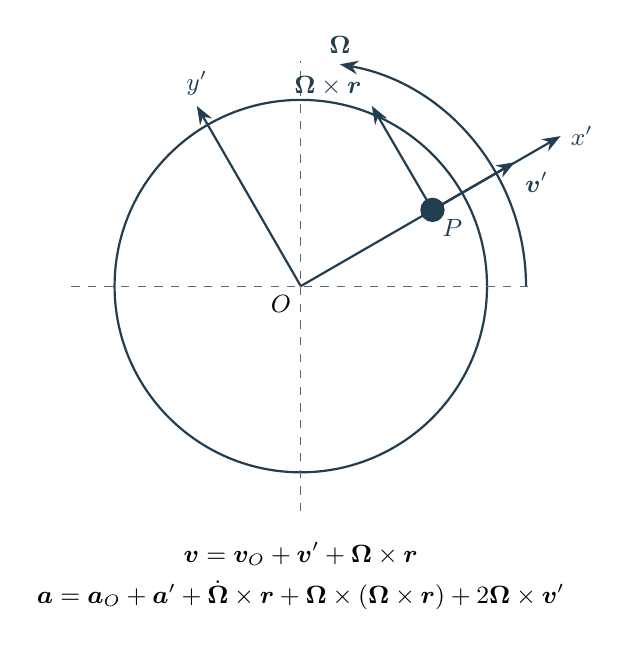
\begin{tikzpicture}[scale=1.1]
\draw[ink,thick](0,0)circle(2.15);
\draw[guide](-2.65,0)--(2.65,0);\draw[guide](0,-2.6)--(0,2.6);
\draw[force](0,0)--(3.0,1.732)node[right]{$x'$};
\draw[force](0,0)--(-1.2,2.08)node[above]{$y'$};
\coordinate(P)at(1.52,.88);\fill[ink](P)circle(4pt)node[below right]{$P$};
\draw[force](P)--++(.95,.55)node[below right]{$\vect v'$};
\draw[force](P)--++(-.7,1.2)node[above left]{$\Om\times\vect r$};
\draw[->,thick,ink](2.6,0)arc(0:80:2.6)node[above]{$\Om$};
\node[below left]at(0,0){$O$};
\node[align=center]at(0,-3.35){$\vect v=\vect v_O+\vect v'+\Om\times\vect r$\\[4pt]
$\vect a=\vect a_O+\vect a'+\dot{\Om}\times\vect r
+\Om\times(\Om\times\vect r)+2\Om\times\vect v'$};
\end{tikzpicture}
\vfill{\normalsize 定义与证明\quad 完整例题\quad 图解分析\quad 练习与解答\par}\vspace{10mm}
\end{titlepage}
\pagenumbering{roman}
\section*{符号与基本约定}
本章研究一个与观察方式有关的力学问题：同一个质点的运动，怎样在惯性系与平动、转动的参考系之间转换？运动学先给出矢量求导、速度和加速度的变换；动力学再将附加的加速度移到力的一侧，建立非惯性系中的运动方程。旋转装置的约束反力、地球上物体的偏转和傅科摆，均由这一条推导链联系起来。

本章采用经典力学和理想约束模型，质量 $m$ 为常数。地球自转问题按明确的量级保留相应阶数；局部有效重力已包含参考点的离心效应，不能再次重复加入同一项。本章以题干规定的坐标与方向为准；插图的记号或转向与正文不同时，图题说明两者的对应。
\begin{center}\small
\begin{tabularx}{\linewidth}{@{}lX@{}}\toprule
记号&含义\\\midrule
$S,S'$&惯性参考系与动参考系\\
$O,O'$&两系原点；原点重合时都记为 $O$\\
$\vect r$&质点相对动系原点的位置矢量\\
$\Om,\dot{\Om}$&动系相对惯性系的角速度与角加速度\\
$\vect v',\vect a'$&相对速度与相对加速度\\
$\vect v_O,\vect a_O$&动系原点的惯性系速度与加速度\\
$\lambda,\Omega_E$&地理纬度与地球自转角速率\\
$\vect e_E,\vect e_N,\vect e_U$&局部向东、向北、向上的右手基矢\\
$f=2\Omega_E\sin\lambda$&水平运动的科氏参数，保留正负号\\\bottomrule
\end{tabularx}\end{center}

\clearpage
\begingroup\small\linespread{1.05}\selectfont
\makeatletter
\renewcommand{\@pnumwidth}{2.2em}\renewcommand{\@tocrmarg}{3.2em}
\renewcommand*\l@section[2]{\addvspace{4pt}\@dottedtocline{1}{0em}{3.4em}{\bfseries #1}{\bfseries #2}}
\renewcommand*\l@subsection{\@dottedtocline{2}{1.5em}{4.2em}}
\makeatother
\tableofcontents\endgroup\clearpage
\pagenumbering{arabic}

\section{转动基矢与矢量求导}\label{sec:c4-1}\label{sec:transport}
\subsection{同一个矢量，两种观察方式}\label{sub:c4-1.1}
设 $S$ 为惯性系，$S'$ 为转动系。先令两个原点重合，只研究坐标轴的转动。$S'$ 的三个单位基矢记为 $\vect e_1,\vect e_2,\vect e_3$，随时间在空间中改变方向，但在 $S'$ 内保持不变。任一空间矢量可以展开为
\[
\vect G=G_1\vect e_1+G_2\vect e_2+G_3\vect e_3.
\]
$G_i(t)$ 是动系中的分量。动系观察者记录分量变化；惯性系观察者还要计入基矢本身的变化。因此“分量不变”与“空间矢量不变”不同。例如固定在转盘上的杆，动系中长度和方向均不变，在惯性系中却不断改变方向。

以下把两种求导写成
\[
\DI\vect G=\sum_i\dot G_i\vect e_i+\sum_iG_i\dot{\vect e}_i,
\qquad
\DR\vect G=\sum_i\dot G_i\vect e_i.
\]
右式并非把矢量变成标量；它仍是空间中的矢量，只是求导规则把动系基矢视为常量。两种导数的差来自同一组基矢的转动。
\TeachingFigure{c4-diagram-01}{固定轴与转动轴对同一空间矢量的分解}
% BEGIN ORIGINAL FIGURES
\OriginalFigure[6.2cm]{c4-1-p002-reference-axes}{空间轴 $\xi,\eta,\zeta$ 与本体轴 $x,y,z$；共同原点为两组三轴交点，体内 $O$ 仅为原图点标记}
% END ORIGINAL FIGURES

\example{动系分量恒定的矢量}\label{ex:c4-1}
\QuestionStatement{惯性系 $S$ 与动系 $S'$ 共用固定原点 $O$。$S'$ 绕共同的竖直轴 $Z$ 以恒角速率 $\Omega>0$ 逆时针转动，$t=0$ 时两系水平轴重合。矢量 $\vect G=G_0\vect e_1$ 固定在动系中，$G_0$ 为常数。求 $(\dd\vect G/\dd t)_S$ 和 $(\dd\vect G/\dd t)_{S'}$，并说明二者为什么不同。}{ex01}{例1题图}
% BEGIN EXPANDED SOLUTION ex01
\solution \Step{先求动系导数}
结合题图\ref{fig:题图-ex01}，解答图\ref{fig:解答图-ex01}展示矢量端点沿圆周移动时的切向导数；$\dot{\vect G}$ 垂直于 $\vect G$，动系中分量仍不变。

动系观察者使用随框架转动的基矢 $\vect e_1,\vect e_2$。题设 $\vect G=G_0\vect e_1$ 中三个动系分量为 $(G_0,0,0)$，均不随时间改变，因此
\[
\left(\frac{\dd\vect G}{\dd t}\right)_{S'}=0.
\]
\SolutionFigure{ex01}

这一步只说明相对框架不变，尚不能判断矢量在空间中是否不变。
\Step{计入基矢转动}
在惯性系中 $\dot{\vect e}_1=\Om\times\vect e_1=\Omega\vect e_2$。由于 $G_0$ 是常量，
\[
\left(\frac{\dd\vect G}{\dd t}\right)_S
=G_0\dot{\vect e}_1=\Omega G_0\vect e_2.
\]
也可用运输定理写成 $0+\Om\times\vect G$，两种计算一致。
\Step{固定坐标中的直接求导}
由初始轴线重合，$\vect e_1=\cos\Omega t\,\vect e_X+\sin\Omega t\,\vect e_Y$。逐项求导得
\[
\dot{\vect G}=G_0\Omega(-\sin\Omega t\,\vect e_X+\cos\Omega t\,\vect e_Y)
=G_0\Omega\vect e_2.
\]
该导数垂直于 $\vect G$，故只改变方向、不改变长度；当 $\Omega\to0$ 时两系导数都为零。

% END EXPANDED SOLUTION ex01
\subsection{从微小转动到基矢的导数}\label{sub:c4-1.2}\label{topic:basis}
在时间 $\dd t$ 内，参考系经历角位移 $\dd\vect\theta=\Om\dd t$。对于任一刚性附着的矢量 $\vect b$，一阶变化为
\[
\dd\vect b=\dd\vect\theta\times\vect b.
\]
可以从几何上检验这一式：沿转轴的分量不变；垂直分量在垂直于轴的圆上移动；切向位移的大小为 $b_\perp\dd\theta$，方向按右手规则确定。除以 $\dd t$，有
\begin{equation}
\dot{\vect e}_i=\Om\times\vect e_i.\label{eq:basis}
\end{equation}
该式允许转轴方向和转速都随时间变化，$\Om$ 是瞬时角速度。只在计算一个瞬间的一阶变化时把它视为给定量，并未假设匀速定轴转动。
\TeachingFigure{c4-diagram-02}{转动矢量端点的透视图；有限端点差为弦，无穷小变化沿垂轴圆的切线}

若某一基矢恰与转轴平行，它的惯性系导数为零，其余两基矢仍会转动。不能由一个基矢不变推断参考系不转动。

\subsection{矢量导数的运输公式}\label{sub:c4-1.3}\label{topic:transport}
将式\eqref{eq:basis}代入逐项求导，
\begin{align*}
\DI\vect G
&=\sum_i\dot G_i\vect e_i+\sum_iG_i(\Om\times\vect e_i)\\
&=\DR\vect G+\Om\times\sum_iG_i\vect e_i.
\end{align*}
于是
\begin{equation}
\DI\vect G=\DR\vect G+\Om\times\vect G.\label{eq:transport}
\end{equation}
这是本章速度、加速度及角动量变换的共同基础。$\vect G$ 可以是位矢、速度、角动量或其他矢量，只要两种导数针对同一个空间矢量且采用同一动系。

叉乘项不是附加的物理变化机制，而是两种观察方式的差异。给定一个在惯性空间不变的矢量，式\eqref{eq:transport}反而给出
\[
\DR\vect G=-\Om\times\vect G.
\]
动系观察者看到它朝参考系转动的反方向改变分量。
\example{惯性空间中固定的水平矢量}\label{ex:c4-2}
\QuestionStatement{两系共用固定原点，动系以 $\Omega\vect e_Z$ 匀速转动，$t=0$ 时 $\vect e_1=\vect e_X$、$\vect e_2=\vect e_Y$。矢量 $\vect G=G_0\vect e_X$ 在惯性空间中恒定。求它在动系中的两个水平分量及动系矢量导数，并用运输定理核验惯性系导数。}{ex02}{例2题图}
% BEGIN EXPANDED SOLUTION ex02
\solution \Step{把固定矢量投影到转动轴}
结合题图\ref{fig:题图-ex02}，解答图\ref{fig:解答图-ex02}展示固定矢量在转动轴上的正、负投影，以及动系导数与基矢转动贡献的抵消；投影中的负号来自 $\vect e_2$ 方向。

框架转角为 $\theta=\Omega t$。由基矢关系
\[
\vect e_1=\cos\theta\,\vect e_X+\sin\theta\,\vect e_Y,
\quad\vect e_2=-\sin\theta\,\vect e_X+\cos\theta\,\vect e_Y,
\]
\SolutionFigure{ex02}

反解得 $\vect e_X=\cos\theta\,\vect e_1-\sin\theta\,\vect e_2$。因此动系分量为
\[
G_1=G_0\cos\Omega t,\qquad G_2=-G_0\sin\Omega t,\qquad G_3=0.
\]
\Step{求动系矢量导数}
求动系导数时只对分量求导，基矢暂视为固定，故
\[
\left(\frac{\dd\vect G}{\dd t}\right)_{S'}
=-\Omega G_0\sin\Omega t\,\vect e_1-\Omega G_0\cos\Omega t\,\vect e_2.
\]
初始时它沿 $-\vect e_2$，符合动系向逆时针转、固定矢量在动系中向顺时针转的几何图像。
\Step{运输公式的分量展开}
另有
\[
\Om\times\vect G
=\Omega G_0\sin\Omega t\,\vect e_1+\Omega G_0\cos\Omega t\,\vect e_2.
\]
两项逐分量抵消，得到 $(\dd\vect G/\dd t)_S=0$。本题与前一例恰好相反：固定的是惯性分量，动系分量必然变化。

% END EXPANDED SOLUTION ex02
\subsection{旋转矩阵与角速度的反对称矩阵}\label{sub:c4-1.4}\label{topic:matrix}
将动系基矢在惯性系中的分量排列为矩阵 $Q(t)$ 的三列，$Q^{\mathsf T}Q=I$、$\det Q=1$。动系分量列向量记为 $\vect G'$，惯性系分量为 $\vect G_S$，则
\[
\vect G_S=Q\vect G',\qquad
\dot{\vect G}_S=Q\dot{\vect G}'+\dot Q\vect G'.
\]
对正交关系求导，
\[
\dot Q Q^{\mathsf T}+Q\dot Q^{\mathsf T}=0.
\]
因此 $W=\dot Q Q^{\mathsf T}$ 是反对称矩阵。任一三阶反对称矩阵可唯一写成某矢量的叉乘算子：
\[
W=[\Om]_\times=
\begin{pmatrix}
0&-\Omega_Z&\Omega_Y\\
\Omega_Z&0&-\Omega_X\\
-\Omega_Y&\Omega_X&0
\end{pmatrix},\qquad W\vect G_S=\Om\times\vect G_S.
\]
于是矩阵求导直接恢复式\eqref{eq:transport}。空间分量形式为 $\dot Q=[\Om]_\times Q$；本体分量形式为 $\dot Q=Q[\Om']_\times$，其中 $\Om'=Q^{\mathsf T}\Om$。两式不能在不变换分量的情况下交换左右乘法。
\example{平面转动矩阵的直接核验}\label{ex:c4-3}
\QuestionStatement{动系相对惯性系绕共同的 $Z$ 轴转过角度 $\theta(t)$，正向按右手定则规定。动系分量到惯性系分量的变换矩阵为
\[Q=\begin{pmatrix}\cos\theta&-\sin\theta&0\\\sin\theta&\cos\theta&0\\0&0&1\end{pmatrix}.\]
直接计算 $\dot Q Q^{\mathsf T}$，由其反对称结构确定瞬时角速度。讨论该结论是否要求匀速转动。}{ex03}{例3题图}
% BEGIN EXPANDED SOLUTION ex03
\solution \Step{分别求导与转置}
结合题图\ref{fig:题图-ex03}，解答图\ref{fig:解答图-ex03}展示两个水平基矢的导数分别沿正 $\vect e_2$ 与负 $\vect e_1$；竖轴导数为零并不排除沿竖轴的角速度。

记 $c_\theta=\cos\theta$、$s_\theta=\sin\theta$。链式法则给出
\[
\dot Q=\dot\theta\begin{pmatrix}-s_\theta&-c_\theta&0\\c_\theta&-s_\theta&0\\0&0&0\end{pmatrix},
\qquad Q^{\mathsf T}=\begin{pmatrix}c_\theta&s_\theta&0\\-s_\theta&c_\theta&0\\0&0&1\end{pmatrix}.
\]
\SolutionFigure{ex03}

\Step{逐项相乘识别角速度}
例如乘积的 $(1,1)$ 元为 $\dot\theta(-s_\theta c_\theta+c_\theta s_\theta)=0$，$(1,2)$ 元为 $-\dot\theta(s_\theta^2+c_\theta^2)=-\dot\theta$。其余项同理，
\[
\dot Q Q^{\mathsf T}=\begin{pmatrix}0&-\dot\theta&0\\\dot\theta&0&0\\0&0&0\end{pmatrix}.
\]
与一般叉乘矩阵 $[\Om]_\times$ 对照，可读出 $\Omega_X=\Omega_Y=0$、$\Omega_Z=\dot\theta$，即 $\Om=\dot\theta\vect e_Z$。
\Step{说明适用条件}
推导只使用了 $\theta(t)$ 的一阶导数，没有令 $\ddot\theta=0$，所以也适用于非匀速定轴转动。若 $\dot\theta$ 改变符号，转向也随之改变。矩阵 $\dot Q Q^{\mathsf T}$ 的量纲为时间的倒数，与角速度一致。

% END EXPANDED SOLUTION ex03
\subsection{正交性的保持与瞬时角速度的唯一性}\label{sub:c4-1.5}\label{topic:orthogonality}
三个基矢共有九个分量，但正交归一条件给出六个独立限制，余下三个自由度正好对应瞬时转动。由式\eqref{eq:basis}，
\[
\frac{\dd}{\dd t}(\vect e_i\cdot\vect e_j)
=(\Om\times\vect e_i)\cdot\vect e_j+\vect e_i\cdot(\Om\times\vect e_j)=0.
\]
因此旋转演化保持基矢夹角与长度。反过来，任何连续变化的正交右手框架，其 $\dot Q Q^{\mathsf T}$ 都是反对称矩阵，唯一对应一个角速度矢量。这个结论把“选参考系”化为可计算的几何对象，而不必真的造出一只刚架。

瞬时角速度可由三个基矢的变化率直接恢复：
\[
\Om=\frac12\sum_{i=1}^3\vect e_i\times\dot{\vect e}_i.
\]
证明时用 $\vect e_i\times(\Om\times\vect e_i)=\Om-(\Om\cdot\vect e_i)\vect e_i$，求和得 $3\Om-\Om=2\Om$。仅给出一根轴的方向变化不能确定绕该轴自转的分量，必须同时说明另外两根轴的选择。

\example{相同竖轴方向不代表相同参考系}\label{ex:c4-4}
\QuestionStatement{两个正交框架共用固定原点与竖轴 $\vect e_3=\vect E_Z$。框架甲的水平轴固定，框架乙的水平轴以恒角速率 $\Omega$ 绕 $Z$ 轴转动。已知两者都有 $\dot{\vect e}_3=0$，能否据此认定两个框架相同？分别写出它们的角速度，并说明仅给一根轴的方向为何不够。}{ex04}{例4题图}
% BEGIN EXPANDED SOLUTION ex04
\solution \Step{给出两个框架的实际差别}
结合题图\ref{fig:题图-ex04}，解答图\ref{fig:解答图-ex04}展示两个水平基矢的导数分别沿正 $\vect e_2$ 与负 $\vect e_1$；竖轴导数为零并不排除沿竖轴的角速度。

框架甲的三个轴都固定，所以它的基矢导数均为零，角速度为 $\Om_{\text{甲}}=0$。框架乙虽然保持同一根竖轴，却有
\[
\dot{\vect e}_1=\Omega\vect e_2,\qquad
\dot{\vect e}_2=-\Omega\vect e_1,\qquad \dot{\vect e}_3=0.
\]
\SolutionFigure{ex04}

因此只比较竖轴导数，无法区分甲、乙。
\Step{从角速度公式说明原因}
由 $\dot{\vect e}_3=\Om\times\vect e_3=0$，只能推出 $\Om$ 平行于 $\vect e_3$ 或为零，不能推出角速度必为零。沿竖轴方向的任意角速度分量都不会改变这根轴本身。
\Step{恢复乙框架的角速度}
用三根基矢共同恢复，
\[
\Om_{\text{乙}}=\frac12\sum_i\vect e_i\times\dot{\vect e}_i
=\frac12\bigl(\Omega\vect e_1\times\vect e_2-\Omega\vect e_2\times\vect e_1\bigr)
=\Omega\vect e_3.
\]
所以两框架并不相同。指定参考系时，除轴向外，还必须交代水平轴绕该轴如何转动。

% END EXPANDED SOLUTION ex04
\subsection{角速度自身的求导与多级参考系}\label{sub:c4-1.6}
把 $\vect G$ 取为 $\Om$，式\eqref{eq:transport}给出
\[
\DI\Om=\DR\Om+\Om\times\Om=\DR\Om.
\]
因此同一参考系的角速度矢量在惯性系与该动系中的一阶矢量导数相同。这里相同的是矢量，坐标分量仍须用 $Q$ 转换。对于另一个矢量，例如刚体相对该系的角速度，叉乘项一般并不为零。

设中间参考系 $S_1$ 相对 $S$ 的角速度为 $\Om_1$，$S_2$ 相对 $S_1$ 的角速度为 $\Om_{21}$。把两者表示为同一组空间分量，依次应用运输公式，得到
\[
\Om_2=\Om_1+\Om_{21}.
\]
对它求惯性系导数时，$\Om_{21}$ 的 $S_1$ 导数还需转换：
\[
\dot{\Om}_2=\dot{\Om}_1+
\left(\frac{\dd\Om_{21}}{\dd t}\right)_{S_1}
+\Om_1\times\Om_{21}.
\]
“角速度相加”不代表“各参考系测得的角加速度分量直接相加”。这也是选用只随进动转动、而不随刚体自转的中间框架时必须注意的区别。
角速度属于参考系之间的相对运动。动系可以由数学上的三根正交坐标轴定义，未必必须固定在某一完整物体上。

\section{速度与加速度的完整变换}\label{sec:c4-2}\label{sec:transform}
\subsection{原点重合时的速度合成}\label{sub:c4-2.1}\label{topic:velocity}
质点相对共同原点的位置为 $\vect r=x\vect e_1+y\vect e_2+z\vect e_3$。在动系中定义
\[
\vect v'=\DR\vect r=\dot x\vect e_1+\dot y\vect e_2+\dot z\vect e_3.
\]
惯性系速度为 $\vect v=\DI\vect r$，由运输公式，
\begin{equation}
\vect v=\vect v'+\Om\times\vect r.\label{eq:velocity}
\end{equation}
$\Om\times\vect r$ 称为牵连速度，表示动系中该瞬时位置的框架点在惯性系的速度。它依赖位置；不同于纯平动时全空间各框架点具有相同牵连速度。
% BEGIN ORIGINAL FIGURES
\OriginalFigure[6.2cm]{c4-2-p001-common-origin}{共原点的惯性轴与转动轴；红色 $\vect r$ 表示同一空间位置矢量}
% END ORIGINAL FIGURES


若质点恰固定在动系中，$\vect v'=0$，式\eqref{eq:velocity}退化为刚体定点运动的速度式。一般运动质点不必是框架的一部分，例如旋转管中的滑块或转盘上自由滑动的小球。
\TeachingFigure{c4-diagram-03}{绝对、相对与牵连速度的平行四边形；分量方向须先统一}

\subsection{逐项求导得到加速度}\label{sub:c4-2.2}\label{topic:acceleration}
对式\eqref{eq:velocity}求惯性系导数。第一项 $\vect v'$ 本身在动系中变化，同时随基矢转动：
\[
\DI\vect v'=\DR\vect v'+\Om\times\vect v'
=\vect a'+\Om\times\vect v'.
\]
第二项用乘积求导，并将位矢导数替换为速度合成式：
\begin{align*}
\DI(\Om\times\vect r)
&=\dot{\Om}\times\vect r+\Om\times\vect v\\
&=\dot{\Om}\times\vect r+\Om\times\vect v'
+\Om\times(\Om\times\vect r).
\end{align*}
将两式相加，
\begin{equation}
\vect a=\vect a'+\dot{\Om}\times\vect r
+\Om\times(\Om\times\vect r)+2\Om\times\vect v'.\label{eq:accel}
\end{equation}
两个 $\Om\times\vect v'$ 分别来自相对速度矢量的基矢变化和牵连速度的空间变化。科氏项系数为 $2$，不能在推导中只保留其中一项。

相对加速度为 $\vect a'=\ddot x\vect e_1+\ddot y\vect e_2+\ddot z\vect e_3$。牵连加速度与科氏加速度分别为
\[
\vect a_t=\dot{\Om}\times\vect r+\Om\times(\Om\times\vect r),
\qquad \vect a_c=2\Om\times\vect v'.
\]
只有角速度矢量在惯性空间不变时，才有 $\dot{\Om}=0$。仅有角速率的模不变，而转轴改变方向，仍可能有角加速度项。
% BEGIN ORIGINAL FIGURES
\OriginalFigure[6.2cm]{c4-1-p023-axis-distance}{质点 $P$ 到转轴的垂足为 $M$，距轴距离 $R=r\sin\theta$；这里 $R$ 表示正文 $R_\perp$}
% END ORIGINAL FIGURES

\example{沿旋转径向轴匀速滑动}\label{ex:c4-5}
\QuestionStatement{一根水平径向直管绕固定竖轴 $OZ$ 以恒角速率 $\Omega>0$ 转动。取沿管向外为 $\vect e_1$，逆时针切向为 $\vect e_2$。质点由装置控制，按 $r(t)=r_0+ut$ 沿管向外匀速滑动，其中 $u>0$、$r_0\ge0$。求惯性系加速度的径向与切向分量，并解释相对加速度为零时绝对加速度为何不为零。}{ex05}{例5题图}
% BEGIN EXPANDED SOLUTION ex05
\solution \Step{写出相对运动与框架运动}
结合题图\ref{fig:题图-ex05}，解答图\ref{fig:解答图-ex05}展示珠子处向轴加速度与科氏加速度的正交分解；相对加速度虽为零，这两个附加项仍然存在。

取随管转动的 $\vect e_1$ 沿管向外，$\vect e_2=\vect e_z\times\vect e_1$。由 $r=r_0+ut$，有
\[
\vect r=r\vect e_1,\quad\vect v'=u\vect e_1,\quad\vect a'=0,
\quad\Om=\Omega\vect e_z,\quad\dot\Om=0.
\]
\SolutionFigure{ex05}

原点固定，所以没有平动加速度项。
\Step{计算两个非零附加项}
利用 $\vect e_z\times\vect e_1=\vect e_2$、$\vect e_z\times\vect e_2=-\vect e_1$，
\[
\Om\times(\Om\times\vect r)=-\Omega^2r\vect e_1,
\qquad 2\Om\times\vect v'=2\Omega u\vect e_2.
\]
从而绝对加速度为
\[
\vect a=-\Omega^2(r_0+ut)\vect e_1+2\Omega u\vect e_2.
\]
径向分量指向转轴，切向分量沿转动正向。
\Step{结果与模型范围}
在固定坐标中写 $\vect r=(r_0+ut)(\cos\Omega t\,\vect e_X+\sin\Omega t\,\vect e_Y)$，二次求导也得到上述两项。$u=0$ 时退化为盘上固定点的向心加速度；$\Omega=0$ 时加速度为零。这里的匀速滑动由装置控制，不能直接当作无沿管力的自由珠运动。

% END EXPANDED SOLUTION ex05
\subsection{向轴分量与空间转动的几何}\label{sub:c4-2.3}\label{topic:axial}
利用三重积恒等式，
\[
\Om\times(\Om\times\vect r)
=(\Om\cdot\vect r)\Om-\Omega^2\vect r.
\]
当 $\Omega\ne0$，定义 $\vect n=\Om/\Omega$，将位矢分为沿轴与垂轴分量：
\[
\vect r_\parallel=(\vect r\cdot\vect n)\vect n,
\qquad \vect R_\perp=\vect r-\vect r_\parallel.
\]
于是
\begin{equation}
\Om\times(\Om\times\vect r)=-\Omega^2\vect R_\perp.\label{eq:centripetal}
\end{equation}
$\vect R_\perp$ 从转轴指向质点，而 $\vect r$ 从动系原点指向质点。空间运动中两者通常不同。向轴加速度指向转轴，模为 $\Omega^2R_\perp$；只有位矢完全位于垂轴平面中时才能写成 $-\Omega^2\vect r$。
\TeachingFigure{c4-diagram-04}{三维转动的向轴项使用垂轴分量，而非整个位置矢量}
% BEGIN ORIGINAL FIGURES
\OriginalFigure[6.2cm]{c4-1-p018-axial-projection}{位矢与转轴的垂直分量；原图 $\vect R$ 对应正文 $\vect R_\perp$，$\vect\omega$ 对应 $\Om$}
% END ORIGINAL FIGURES

$\Omega=0$ 的瞬间不宜用 $\vect n=\Om/\Omega$ 定义轴；原叉乘式始终有效，且向轴项为零。

\subsection{原点平动并同时转动的动系}\label{sub:c4-2.4}\label{topic:generalframe}
设动系原点 $O'$ 在惯性系中的位置为 $\vect r_O$，质点绝对位置为
\[
\vect R=\vect r_O+\vect r.
\]
先把两系原点的相对平动分离，再对 $\vect r$ 应用运输公式，得
\begin{align}
\vect v=\vect v_O+\vect v'+\Om\times\vect r,\label{eq:generalv}\\
\vect a=\vect a_O+\vect a'+\dot{\Om}\times\vect r
+\Om\times(\Om\times\vect r)+2\Om\times\vect v'.\label{eq:generala}
\end{align}
其中 $\vect r$ 必须相对 $O'$ 定义。将绝对位置 $\vect R$ 错代入旋转项，会把原点的位置计入两次。

\subsubsection*{通过中间平动系逐步得到通式}
构造原点为 $O'$、坐标轴始终平行于惯性系的中间系 $S''$。它只作平动，不随 $S'$ 转动。先由位置差求导：
\[
\vect v=\vect v_O+\vect v'',\qquad
\vect a=\vect a_O+\vect a''.
\]
再比较共同原点的 $S''$ 与 $S'$，由式\eqref{eq:velocity}和\eqref{eq:accel}，
\[
\vect v''=\vect v'+\Om\times\vect r,
\quad
\vect a''=\vect a'+\dot\Om\times\vect r
+\Om\times(\Om\times\vect r)+2\Om\times\vect v'.
\]
将第二组代入第一组便得通式。中间系 $S''$ 在原点加速时也不是惯性系，但这里使用的是位置与基矢求导的运动学恒等式，并未在其中无条件应用惯性系牛顿定律。此构造也说明为什么原点加速度只出现一次。

\TeachingFigure{c4-diagram-05}{一般动系的位置三角形：平动项与转动项使用不同位置矢量}
\example{加速小车上的转动径向管}\label{ex:c4-6}
\QuestionStatement{小车上的原点 $O'$ 沿惯性 $X$ 方向以加速度 $A$ 平动。一根水平直管绕 $O'$ 以恒角速率 $\Omega>0$ 转动，当前管轴与 $X$ 轴夹角为 $\theta$。质点距 $O'$ 为 $r$，以恒定相对速率 $u$ 沿管向外滑动。取沿管为 $\vect e_1$、正切向为 $\vect e_2$，求绝对加速度的两个分量。}{ex06}{例6题图}
% BEGIN EXPANDED SOLUTION ex06
\solution \Step{先在动系基矢上列完整矢量式}
结合题图\ref{fig:题图-ex06}，解答图\ref{fig:解答图-ex06}展示珠子处向轴加速度与科氏加速度的正交分解，并单独投影原点平动加速度；先统一基矢再相加。

原点加速度为 $A\vect e_X$，管角速度恒定，珠子的相对加速度为零。故
\[
\vect a=A\vect e_X-\Omega^2r\vect e_1+2\Omega u\vect e_2.
\]
\SolutionFigure{ex06}

此式已经区分原点平动、向轴加速度与科氏加速度，不能把第一项并入半径 $r$。
\Step{投影原点加速度}
因为 $\vect e_1$ 与 $X$ 轴夹角为 $\theta$，而 $\vect e_2$ 是其逆时针转 $90^\circ$ 的方向，
\[
\vect e_X=\cos\theta\,\vect e_1-\sin\theta\,\vect e_2.
\]
于是
\[
a_1=A\cos\theta-\Omega^2r,\qquad a_2=-A\sin\theta+2\Omega u.
\]
\Step{方向约定与计算结果}
$-\Omega^2r$ 总沿管向轴内；向外相对运动产生正切向科氏加速度。小车向固定 $X$ 方向加速，其在旋转管轴上的投影则随 $\theta$ 改变。$A=0$ 时恢复固定轴径向管结果；$\theta=0$ 时小车加速度只有沿管分量，切向分量仍为 $2\Omega u$。

% END EXPANDED SOLUTION ex06
\subsection{平面变换的分量与复数形式}\label{sub:c4-2.5}\label{topic:planar}
取 $\Om=\Omega(t)\vect e_z$，质点在动系 $xy$ 平面内运动。由式\eqref{eq:generala}，忽略原点平动时
\begin{align}
a_x&=\ddot x-2\Omega\dot y-\dot\Omega y-\Omega^2x,\\
a_y&=\ddot y+2\Omega\dot x+\dot\Omega x-\Omega^2y.
\end{align}
这是绝对加速度在动系基矢上的分量，不是动系中坐标的二阶导数。定义复数 $z=x+\mathrm iy$，框架转角 $\theta$ 满足 $\dot\theta=\Omega$，绝对复位置为 $Z=e^{\mathrm i\theta}z$。直接求导，
\[
\dot Z=e^{\mathrm i\theta}(\dot z+\mathrm i\Omega z),
\]
\[
\ddot Z=e^{\mathrm i\theta}
\bigl[\ddot z+2\mathrm i\Omega\dot z
+(\mathrm i\dot\Omega-\Omega^2)z\bigr].
\]
实部与虚部恢复上述分量式。复数乘以 $\mathrm i$ 对应在平面内逆时针转 $90^\circ$，因而它自然代表与 $\vect e_z$ 的叉乘。
复数法仅适用于已明确的平面转动，不能用一个复数替代任意三维转轴变化。

\subsection{特殊情形与参数极限}\label{sub:c4-2.6}
通用式\eqref{eq:generala}应通过以下检验：
\begin{enumerate}
\item 纯平动 $\Om=0$：$\vect a=\vect a_O+\vect a'$。
\item 动系固定点 $\vect v'=\vect a'=0$：只剩原点和框架点的加速度。
\item 匀速定轴转动 $\dot{\Om}=0$：角加速度项消失，向轴与科氏项仍存在。
\item 相对运动沿转轴：$\Om\times\vect v'=0$，但离轴位置仍可有向轴项。
\item 相对静止不代表绝对静止：$\vect v'$ 为零不保证 $\vect v$ 为零。
\end{enumerate}
四个附加加速度项的量纲均为长度除以时间平方。$\dot{\Om}\times\vect r$ 关于角加速度一阶，科氏项关于角速度和相对速率分别一阶，向轴项关于角速度二阶；这一区分对地球自转的微扰分析尤为重要。
\example{科氏项为零的三种情形}\label{ex:c4-7}
\QuestionStatement{动系角速度为 $\Om$，质点的相对速度为 $\vect v'$，科氏加速度为 $2\Om\times\vect v'$。分别考察：参考系不转动；质点固定在动系；质点相对运动平行于转轴。判断每种情况下科氏项是否为零，并给出科氏项消失的统一条件。相对速率恒定或相对轨迹为直线，是否已足够？}{ex07}{例7题图}
% BEGIN EXPANDED SOLUTION ex07
\solution \Step{先写模长条件}
结合题图\ref{fig:题图-ex07}，解答图\ref{fig:解答图-ex07}展示相对速度平行转轴时的零叉乘，以及垂直转轴时的非零叉乘；判断依据是夹角而非轨迹是否为直线。

设 $\alpha$ 为 $\Om$ 与 $\vect v'$ 的夹角，则
\[
a_c=2|\Om\times\vect v'|=2\Omega v'|\sin\alpha|.
\]
\SolutionFigure{ex07}

叉乘为零的充要条件是其中一个矢量为零，或者两个非零矢量平行或反平行。
\Step{逐种判断题设情形}
参考系不转动时 $\Om=0$，没有科氏项；质点固定于动系时 $\vect v'=0$，也没有科氏项；沿转轴运动时 $\vect v'\parallel\Om$，即使相对速率不为零，科氏项仍为零。三种情形均符合上述统一条件。
\Step{转轴与基矢的几何关系}
相对速率恒定只限制 $v'$ 的大小，并不限制它与转轴的夹角。沿水平径向管匀速外滑就是反例：相对轨迹为直线、速率恒定，却有 $a_c=2\Omega u$。同样，“没有主动力”也不保证科氏项为零。判断时应直接检查叉乘中的两个矢量。

% END EXPANDED SOLUTION ex07
\section{旋转装置的运动学分析}\label{sec:c4-3}\label{sec:kinmodels}
\subsection{转动直管中的匀速质点}\label{sub:c4-3.1}\label{topic:radialkin}
\example{两处半径的绝对速度与加速度}\label{ex:c4-8}
\QuestionStatement{一根长度为 $R$ 的水平直管，一端 $O$ 位于固定竖直转轴上，管以恒角速率 $\Omega>0$ 逆时针转动。质点受控制，以相对速率 $u>0$ 沿管向外匀速移动。分别求其经过 $r=R/3$ 和管端 $r=R$ 时的绝对速度、速率及绝对加速度，并判断惯性平面内的轨迹形状。为确定轨迹的具体位置，设初始时刻 $r(0)=r_0$、管轴方位角为 $\theta_0$，其中 $0\le r_0<R/3$；只讨论质点尚未离开管端的过程。}{ex08}{例8题图}
% BEGIN EXPANDED SOLUTION ex08
\solution \Step{速度由两个正交分量合成}
结合题图\ref{fig:题图-ex08}，解答图\ref{fig:解答图-ex08}展示速度三角形与加速度矩形；两位置的牵连速度及向轴加速度随 $r$ 改变，而科氏分量保持相同。

取径向、切向基矢为 $\er,\et$。相对速度为 $u\er$，牵连速度为 $\Omega r\et$，因此
\[
\vect v=u\er+\Omega r\et,\quad v=\sqrt{u^2+\Omega^2r^2},\quad
\tan\beta=\frac{\Omega r}{u}.
\]
\SolutionFigure{ex08}

这里 $\beta$ 是绝对速度与向外径向的夹角。两位置分别为
\begin{align*}
\vect v_{R/3}&=u\er+\frac{\Omega R}{3}\et,& v_{R/3}&=\sqrt{u^2+\frac{\Omega^2R^2}{9}},\\
\vect v_R&=u\er+\Omega R\et,&v_R&=\sqrt{u^2+\Omega^2R^2}.
\end{align*}
\Step{加速度要计入科氏项}
因为 $\dot r=u$ 恒定，相对加速度为零，但管的转动仍给出
\[
\vect a=-\Omega^2r\er+2\Omega u\et.
\]
所以
\begin{align*}
\vect a_{R/3}&=-\frac{\Omega^2R}{3}\er+2\Omega u\et,\\
\vect a_R&=-\Omega^2R\er+2\Omega u\et,\qquad
|\vect a|=\sqrt{\Omega^4r^2+4\Omega^2u^2}.
\end{align*}
两位置的科氏分量相等，向轴分量却与半径成正比。
\Step{消去时间求轨迹}
由 $r=r_0+ut$、$\theta=\theta_0+\Omega t$，消去 $t$ 得
\[
r=r_0+\frac{u}{\Omega}(\theta-\theta_0).
\]
这是阿基米德螺线的一段。因而管中所见的匀速直线运动，在惯性系中既不是直线，也不是恒速运动。

% END EXPANDED SOLUTION ex08

% BEGIN ORIGINAL FIGURES
\OriginalFigure[6.2cm]{c4-1-p012-rotating-tube}{旋转直管中的质点；图示为动、静轴瞬时对齐的位置，$\omega$ 对应正文 $\Omega$}
% END ORIGINAL FIGURES

\TeachingFigure{c4-diagram-06}{匀速沿管滑动的速度与加速度；两幅图的箭长仅表示分量方向}
本题给定 $u$ 为常量，是运动学规定。光滑管中自由小球的 $u(t)$ 通常并不恒定，必须另解动力学方程。

\subsection{绝对速率恒定时的径向运动}\label{sub:c4-3.2}\label{topic:constantspeed}
\example{旋转射线上的恒绝对速率运动}\label{ex:c4-9}
\QuestionStatement{水平直管绕固定竖轴 $O$ 以恒角速率 $\Omega>0$ 转动，取管轴与固定 $X$ 轴的初始夹角为零。质点在 $t=0$ 从 $O$ 出发，装置控制其惯性系速率始终等于常数 $c$，且最初沿管向外运动。求 $r(t)$、$\dot r(t)$、首个向外阶段的终止时间与最大半径，并确定该阶段的惯性系轨迹。}{ex09}{例9题图}
% BEGIN EXPANDED SOLUTION ex09
\solution \Step{用绝对速率约束求径向方程}
结合题图\ref{fig:题图-ex09}，解答图\ref{fig:解答图-ex09}展示首个向外阶段的惯性系半圆轨迹；半径 $OP$ 在末点达到 $c/\Omega$，而绝对速度在整个过程中仍为切向且大小为 $c$。

绝对速度为 $\dot r\er+\Omega r\et$，两分量正交。规定 $|\vect v|=c$，即
\[
\dot r^2+\Omega^2r^2=c^2.
\]
\SolutionFigure{ex09}

最初向外运动，须选 $\dot r=+\sqrt{c^2-\Omega^2r^2}$；这个符号只适用于首个向外阶段。
\Step{积分并施加初条件}
分离变量并由 $r(0)=0$ 定积分，
\[
\int_0^{r(t)}\frac{\dd q}{\sqrt{c^2-\Omega^2q^2}}=t,
\qquad \arcsin\frac{\Omega r}{c}=\Omega t.
\]
因此
\begin{equation}
r(t)=\frac c\Omega\sin\Omega t,\quad\dot r=c\cos\Omega t,
\quad 0\le t\le\frac\pi{2\Omega}.\label{eq:constspeed}
\end{equation}
在 $t_*=\pi/(2\Omega)$ 时，$\dot r=0$、$r_{\max}=c/\Omega$，全部绝对速度都成为切向分量。不能超过此时仍沿用“向外”的正平方根分支。
\Step{还原惯性系中的轨迹}
初始轴重合，$X=r\cos\Omega t$、$Y=r\sin\Omega t$，于是
\[
X=\frac{c}{2\Omega}\sin2\Omega t,\qquad
Y=\frac{c}{2\Omega}(1-\cos2\Omega t).
\]
消去时间得 $X^2+(Y-c/(2\Omega))^2=(c/(2\Omega))^2$。首个向外阶段对应 $X\ge0$ 的半圆，从原点到 $(0,c/\Omega)$；这也说明径向速度变为零并不代表质点绝对停止。

% END EXPANDED SOLUTION ex09

% BEGIN ORIGINAL FIGURES
\OriginalFigure[6.2cm]{c4-1-p013-constant-speed}{固定轴 $x,y$ 与沿直线转动的轴 $x^{\prime},y^{\prime}$；管上坐标对应正文 $r$，角速率 $\omega$ 对应 $\Omega$}
% END ORIGINAL FIGURES

\subsubsection*{惯性轨迹的几何}
在首个向外阶段 $\theta=\Omega t$，惯性直角坐标为
\[
X=r\cos\theta=\frac{c}{2\Omega}\sin2\Omega t,
\quad
Y=r\sin\theta=\frac{c}{2\Omega}(1-\cos2\Omega t).
\]
所以
\[
X^2+\left(Y-\frac{c}{2\Omega}\right)^2
=\left(\frac{c}{2\Omega}\right)^2.
\]
首段绝对轨迹是一段半圆，半径 $c/(2\Omega)$；绝对角速率为 $2\Omega$，惯性速率为 $c$，与题设一致。角度已经转动而相对径向速度恰为零的时刻，对应半圆另一端。
\TeachingFigure{c4-diagram-07}{恒绝对速率运动的首个向外阶段在惯性系中成为半圆}
固定 $t$ 并令 $\Omega\to0$ 时，$r(t)\to ct$，圆半径趋于无穷，轨迹在有限范围内趋于直线。

\subsection{离心调速器小球的速度}\label{sub:c4-3.3}\label{topic:governorkin}
调速器小球由长度为 $l$ 的杆连接到轴上悬点。杆与向下竖直方向夹角为 $\theta(t)$，框架绕竖直轴以角速率 $\Omega(t)$ 转动。选择只随框架方位转动的动系，$\vect e_r$ 指向水平外侧，$\vect e_\theta$ 沿方位角增大方向，$\vect e_z$ 竖直向上。
\[
\vect r=l\sin\theta\vect e_r-l\cos\theta\vect e_z,
\qquad \Om=\Omega\vect e_z.
\]
小球相对速度为
\[
\vect v'=l\dot\theta\cos\theta\vect e_r
+l\dot\theta\sin\theta\vect e_z.
\]
它处于包含轴的竖直子午面内；第二项属于竖直方向。牵连速度沿方位方向：
\[
\vect v_t=\Omega l\sin\theta\vect e_\theta.
\]
故
\begin{equation}
\vect v=l\dot\theta\cos\theta\vect e_r
+\Omega l\sin\theta\vect e_\theta
+l\dot\theta\sin\theta\vect e_z.\label{eq:governorv}
\end{equation}
三分量正交，
\[
v^2=l^2\dot\theta^2+\Omega^2l^2\sin^2\theta.
\]
相对平衡 $\dot\theta=0$ 时，小球仍以速率 $\Omega l\sin\theta$ 绕轴作圆周运动。
\TeachingFigure{c4-diagram-08}{调速器小球的子午面侧视图；相对速度在纸面内，牵连速度垂直纸面}
% BEGIN ORIGINAL FIGURES
\OriginalFigure[6.2cm]{c4-1-p015-governor-velocity}{调速器小球的相对摆动速度；$\vect i,\vect j,\vect k$ 分别对应正文 $\vect e_r,\vect e_\theta,\vect e_z$，竖直分量沿 $\vect k$}
% END ORIGINAL FIGURES

\example{给定摆角与摆角速度的调速器}\label{ex:c4-10}
\QuestionStatement{离心调速器的小球由长 $l$ 的轻杆与转轴上的固定铰点相连。轻杆所在的竖直平面以恒角速率 $\Omega$ 绕轴转动；杆与向下竖直线的夹角为 $\theta$，并以角速度 $\dot\theta$ 在该平面内摆动。在某时刻，$l=0.50\,\mathrm m$、$\theta=30^\circ$、$\dot\theta=0.20\,\mathrm{s^{-1}}$、$\Omega=6.0\,\mathrm{s^{-1}}$。求小球相对速率、牵连速率及惯性系速率。小球视为质点；图中质量记为 $m$，本题速度结果不依赖 $m$。}{ex10}{例10题图}
% BEGIN EXPANDED SOLUTION ex10
\solution \Step{分别识别两种运动}
结合题图\ref{fig:题图-ex10}，解答图\ref{fig:解答图-ex10}展示相对速度与牵连速度的正交三角形；前者来自杆在子午面内摆动，后者来自小球绕竖轴的转动。

在只随调速器绕竖轴转动的框架中，小球沿摆角增大的方向运动，相对速率为 $v'=l|\dot\theta|$。其距竖轴的距离为 $\rho=l\sin\theta$，故牵连速率为 $v_t=\Omega\rho$。
\Step{说明为何可以平方相加}
相对速度位于径向竖直平面内，牵连速度沿方位切向，垂直该平面，因而
\[
\vect v'\cdot\vect v_t=0,\qquad
v^2=l^2\dot\theta^2+\Omega^2l^2\sin^2\theta.
\]
\SolutionFigure{ex10}

若不先辨认方向，直接把两个速率相加，会把正交运动误作同向运动。
\Step{数值代入与单位换算}
\[
v'=0.50\times0.20=0.10\,\mathrm{m/s},\quad
\rho=0.50\sin30^\circ=0.25\,\mathrm m,
\]
\[
v_t=6.0\times0.25=1.50\,\mathrm{m/s},\qquad
v=\sqrt{0.10^2+1.50^2}=\sqrt{2.26}\approx1.503\,\mathrm{m/s}.
\]
结果略大于牵连速率，符合较小的正交相对速度只使合速率略有增加的情况。若 $\dot\theta=0$，便退化为小球随框架作定半径圆周运动。

% END EXPANDED SOLUTION ex10
\subsection{调速器的加速度与驱动转矩}\label{sub:c4-3.4}
利用完整变换式，各项为
\begin{align*}
\vect a'&=l(\ddot\theta\cos\theta-\dot\theta^2\sin\theta)\vect e_r
+l(\ddot\theta\sin\theta+\dot\theta^2\cos\theta)\vect e_z,\\
\dot{\Om}\times\vect r&=l\dot\Omega\sin\theta\vect e_\theta,\\
\Om\times(\Om\times\vect r)&=-l\Omega^2\sin\theta\vect e_r,\\
2\Om\times\vect v'&=2l\Omega\dot\theta\cos\theta\vect e_\theta.
\end{align*}
因此
\begin{align}
a_r&=l\ddot\theta\cos\theta-l\dot\theta^2\sin\theta-l\Omega^2\sin\theta,\\
a_\theta&=l\dot\Omega\sin\theta+2l\Omega\dot\theta\cos\theta,\\
a_z&=l\ddot\theta\sin\theta+l\dot\theta^2\cos\theta.
\end{align}
即使 $\Omega$ 恒定，小球向外或向内摆动时仍有方位加速度。它必须由框架的约束力或驱动提供。

关于轴的角动量为 $L_z=m\Omega l^2\sin^2\theta$，故轴向驱动转矩为
\[
\tau_z=\dot L_z=ml^2
\left(\dot\Omega\sin^2\theta+2\Omega\dot\theta\sin\theta\cos\theta\right).
\]
另一方面，方位作用力 $F_\theta=ma_\theta$ 对轴的力矩为 $l\sin\theta F_\theta$，代入同样恢复上式。保持转速恒定不等于驱动转矩恒定，更不等于驱动不做功。
给定 $\Omega(t)$ 的框架运动学，与发动机和阀门共同决定的真实调速过程，是不同的模型。后者还需把转速作为动力学未知量。

\subsection{圆盘圆槽中的同向与反向运动}\label{sub:c4-3.5}\label{topic:circulargroove}
\example{同心圆槽中的绝对加速度}\label{ex:c4-11}
\QuestionStatement{圆盘绕固定中心 $O$ 匀速转动，盘角速度为 $\Omega\vect e_z$。盘上半径为 $a$ 的同心圆槽内，一质点以相对角速度 $\nu\vect e_z$ 匀速运动。$\Omega$ 与 $\nu$ 均为有符号常数，俯视逆时针为正。求质点绝对速度、绝对加速度，并分别列出相对、牵连和科氏加速度。}{ex11}{例11题图}
% BEGIN EXPANDED SOLUTION ex11
\solution \Step{相对运动和框架运动分别计算}
结合题图\ref{fig:题图-ex11}，解答图\ref{fig:解答图-ex11}展示相对向心、牵连向心和有符号科氏分量的径向合成；同向时三项向内，反向时须保留 $\Omega\nu$ 的符号。

槽中心与转轴重合，质点在半径 $a$ 的圆周上，故
\[
\vect v'=a\nu\et,\qquad\vect a'=-a\nu^2\er,
\quad\vect v_t=a\Omega\et,\quad\vect a_t=-a\Omega^2\er.
\]
\SolutionFigure{ex11}

$\Omega,\nu$ 都带符号，而各自的向心加速度包含平方，不随单独转向改变。
\Step{保留科氏项的有符号乘积}
利用 $\vect e_z\times\et=-\er$，
\[
\vect a_c=2\Omega\vect e_z\times(a\nu\et)=-2a\Omega\nu\er.
\]
当两种转动反向时 $\Omega\nu<0$，这项沿径向向外，并非总是向心。
\Step{速度合成与直接微分}
\begin{equation}
\vect v=a(\Omega+\nu)\et,\qquad
\vect a=-a(\Omega+\nu)^2\er.\label{eq:groove}
\end{equation}
惯性系方位角为 $\theta=\theta_0+(\Omega+\nu)t$，所以直接把它视为角速度 $\Omega+\nu$ 的圆周运动，也给出同样答案。$\nu=0$ 时恢复盘上固定点；$\nu=-\Omega$ 时绝对速度、加速度同时为零。

% END EXPANDED SOLUTION ex11
\TeachingFigure{c4-diagram-09}{同心圆槽中必须以有符号角速率合成，反向时科氏项改变符号}
% BEGIN ORIGINAL FIGURES
\OriginalFigure[6.2cm]{c4-1-p022-circular-groove}{圆盘与质点均顺时针运动的情形；图中 $R=a$、$v_r=|\nu|a$、$v_e=|\Omega|a$，对应正文 $\Omega<0,\ \nu<0$}
% END ORIGINAL FIGURES

\example{相对运动存在但质点绝对静止}\label{ex:c4-12}
\QuestionStatement{圆盘绕固定竖轴以角速度 $\Omega\vect e_z$ 匀速转动，质点在半径 $a$ 的同心圆槽内以相对角速度 $\nu=-\Omega$ 运动。求质点在惯性系中的速度和加速度，并逐项核验三项加速度如何抵消。说明“相对运动存在”与“绝对静止”能否同时成立。}{ex12}{例12题图}
% BEGIN EXPANDED SOLUTION ex12
\solution \Step{先合成速度}
结合题图\ref{fig:题图-ex12}，解答图\ref{fig:解答图-ex12}展示取向外为右时的三个加速度矢量；相对与牵连加速度均向内，而反向相对运动产生双倍向外科氏项。

取正切向为逆时针，珠子相对速度为 $-a\Omega\et$，框架牵连速度为 $+a\Omega\et$，所以
\[
\vect v=-a\Omega\et+a\Omega\et=0.
\]
\SolutionFigure{ex12}

由于 $\nu=-\Omega$ 始终成立，惯性方位角保持常数，质点在惯性空间确实停在同一点。
\Step{加速度各项的计算}
相对圆周运动给出 $\vect a'=-a\Omega^2\er$；框架向轴项为 $-a\Omega^2\er$。科氏项为
\[
2\Om\times\vect v'=2\Omega\vect e_z\times(-a\Omega\et)
=+2a\Omega^2\er.
\]
因此
\[
\vect a=(-a\Omega^2-a\Omega^2+2a\Omega^2)\er=0.
\]
\Step{推导的适用范围}
动系观察者仍看到质点沿槽转动，其相对加速度也不为零；这些量不能与绝对量混同。若把科氏项漏掉系数 $2$，或误认为它总向内，就无法得到这个应当严格成立的静止极限。

% END EXPANDED SOLUTION ex12
\subsection{偏心圆槽与多级转动框架}\label{sub:c4-3.6}\label{topic:framechoice}
\example{圆槽中心不在转盘轴上}\label{ex:c4-13}
\QuestionStatement{水平转盘以恒角速度 $\Omega\vect e_z$ 绕固定轴 $O$ 转动。圆槽中心 $C$ 固定在盘上，$\vect{OC}=d\vect e_1$，槽半径为 $a$。质点相对盘绕 $C$ 匀速运动，其相对角位置为 $\psi=\nu t$，其中 $\nu$ 为有符号常数。以盘上基矢表示质点位置，求惯性系加速度，并指出偏心距离 $d$ 带来的附加项。}{ex13}{例13题图}
% BEGIN EXPANDED SOLUTION ex13
\solution \Step{把偏心圆槽拆成两段位置}
结合题图\ref{fig:题图-ex13}，解答图\ref{fig:解答图-ex13}展示位置分解 $\vect{OP}=\vect{OC}+\vect{CP}$ 及两项绝对加速度；偏心槽中心的加速度不能并入相对半径。

令 $\vect e_\rho=\cos\psi\,\vect e_1+\sin\psi\,\vect e_2$ 指向 $CP$，其正切向为 $\vect e_\psi$。则
\[
\vect r=d\vect e_1+a\vect e_\rho,\quad
\vect v'=a\nu\vect e_\psi,\quad\vect a'=-a\nu^2\vect e_\rho.
\]
\SolutionFigure{ex13}

其中 $d\vect e_1$ 在盘上固定，所以不贡献相对速度，却贡献牵连加速度。
\Step{分别计算牵连和科氏项}
所有位置都在水平面内，故
\[
\vect a_t=-\Omega^2d\vect e_1-\Omega^2a\vect e_\rho,
\qquad\vect a_c=-2\Omega\nu a\vect e_\rho.
\]
将三项相加，得到
\[
\vect a=-\Omega^2d\vect e_1-a(\Omega+\nu)^2\vect e_\rho.
\]
\Step{用几何分解解释结果}
第一项正是槽中心 $C$ 绕 $O$ 的加速度；第二项是质点相对移动中心 $C$ 的惯性圆周加速度。只有 $d=0$ 才退化为同心槽公式。即使 $\nu=-\Omega$，第二项为零，中心 $C$ 的运动仍可使质点加速，不能把前一例的绝对静止结论直接搬来。

% END EXPANDED SOLUTION ex13
\TeachingFigure{c4-diagram-10}{偏心圆槽的加速度由槽中心运动与质点绕中心运动合成}

对复杂刚体运动，可以选择只随某一部分转动的框架。若轴线进动、刚体又绕自身轴自转，取框架只随进动时，框架角速度只包含进动部分；自转作为相对运动另计。若取完全固结于刚体的框架，相对运动减少，但框架总角速度必须包含两部分。
\example{改变框架不应改变绝对速度}\label{ex:c4-14}
\QuestionStatement{惯性系 $S$、中间系 $S_1$ 和随体系 $S_2$ 共用固定原点 $O$。$S_1$ 相对 $S$ 的角速度为 $\Om_1$，$S_2$ 相对 $S_1$ 的角速度为 $\Om_{21}$；质点 $P$ 固定在 $S_2$，位置矢量为 $\vect r$。两角速度须用同一空间基矢表示。分别选 $S_1$、$S_2$ 为动系计算 $P$ 的绝对速度，证明两种选择给出相同结果。}{ex14}{例14题图}
% BEGIN EXPANDED SOLUTION ex14
\solution \Step{选择中间框架计算}
结合题图\ref{fig:题图-ex14}，解答图\ref{fig:解答图-ex14}展示两级角速度的首尾合成；$\Om_2=\Om_1+\Om_{21}$ 决定固定于随体系的点速度，两种选系给出同一叉乘。

在 $S_1$ 中，质点随 $S_2$ 转动而具有相对速度
\[
\vect v'_1=\Om_{21}\times\vect r.
\]
\SolutionFigure{ex14}

再加上 $S_1$ 的牵连速度 $\Om_1\times\vect r$，得到
\[
\vect v=(\Om_1+\Om_{21})\times\vect r.
\]
这里所有角速度都必须先表示成同一空间基矢下的矢量。
\Step{改选完全随体框架计算}
因 $P$ 固定在 $S_2$，$\vect v'_2=0$。然而该框架相对惯性系的角速度是总角速度
\[
\Om_2=\Om_1+\Om_{21},
\]
所以仍有 $\vect v=\Om_2\times\vect r$，与前式逐项一致。
\Step{说明常见漏项}
若选择 $S_1$ 却把 $\vect v'_1$ 设为零，就会漏掉第二级转动；若选择 $S_2$ 却只用 $\Om_1$ 作牵连角速度，也会漏掉同一项。框架选择可以改变相对运动与牵连运动的划分，却不能改变同一点的绝对速度。

% END EXPANDED SOLUTION ex14

% BEGIN ORIGINAL FIGURES
\OriginalFigure[6.2cm]{c4-1-p026-wheel-frame}{随轮轴改变方向的框架；轮绕自身轴的转动可作为相对运动另计}
% END ORIGINAL FIGURES



\example{进动框架与完全随体框架的区别}\label{ex:c4-15}
\QuestionStatement{刚体绕固定点 $O$ 运动，对称轴单位矢量为 $\vect n$。该轴与竖直方向夹角 $\alpha$ 保持不变，并以恒角速率 $\Omega_p$ 绕竖直轴进动；刚体还相对进动框架以角速率 $\omega_s$ 绕 $\vect n$ 自转。分别选择进动框架和完全随体框架，写出总角速度，并求轴上位置 $\vect r=h\vect n$ 处材料点的绝对速度。}{ex15}{例15题图}
% BEGIN EXPANDED SOLUTION ex15
\solution \Step{分别说明两个框架如何运动}
结合题图\ref{fig:题图-ex15}，解答图\ref{fig:解答图-ex15}展示总角速度的竖直进动分量与沿对称轴的自转分量；轴上点只有进动的方位速度，图中 $\otimes$ 表示纸面向内。

进动框架只跟着含竖轴与 $\vect n$ 的平面转动，其角速度为 $\Om_f=\Omega_p\vect e_Z$。材料相对该框架还绕 $\vect n$ 转动，角速度为 $\omega_s\vect n$。因此完全随体框架的总角速度为
\[
\vect\omega_B=\Omega_p\vect e_Z+\omega_s\vect n.
\]
\SolutionFigure{ex15}

这是矢量相加，不能把两角速率的模直接相加；具体有
\[
\omega_B^2=\Omega_p^2+\omega_s^2+2\Omega_p\omega_s\cos\alpha.
\]
\Step{在进动框架中计算轴上点速度}
轴上点 $\vect r=h\vect n$ 的相对自转速度为
\[
\vect v'_f=\omega_s\vect n\times(h\vect n)=0.
\]
故其绝对速度为 $\vect v=\Omega_p\vect e_Z\times h\vect n$，速率为 $|\Omega_p|\,|h|\sin\alpha$。该点绕竖轴运动的半径正是 $|h|\sin\alpha$。
\Step{随体系中的角加速度}
在完全随体系中 $\vect v'_B=0$，且
\[
\vect v=\vect\omega_B\times h\vect n
=\Omega_p\vect e_Z\times h\vect n,
\]
因为自转项的叉乘仍为零。这个结论只适用于轴上点，轴外材料点一般受自转影响。

若 $\Omega_p,\omega_s$ 的数值都恒定，轴向仍满足 $\dot{\vect n}=\Omega_p\vect e_Z\times\vect n$，所以
\[
\dot{\vect\omega}_B=\omega_s\Omega_p\vect e_Z\times\vect n.
\]
总角加速度可以非零；计算轴外点加速度时，不能因两个角速率恒定就删去欧拉加速度项。

% END EXPANDED SOLUTION ex15

% BEGIN ORIGINAL FIGURES
\OriginalFigure[6.2cm]{c4-1-p026-precessing-frame}{倾斜轴的自转与进动；$\omega_1$ 对应正文 $\omega_s$，$\omega_2$ 对应 $\Omega_p$}
% END ORIGINAL FIGURES

\TeachingFigure{c4-diagram-11}{倾斜轴刚体的进动与自转；两种框架不能混用角速度}
轮与转轴的组合可采用同样思路：令框架跟随轮轴改变方向，但把轮绕轴的转动留作相对运动；锥体绕定点运动也可选择跟随锥轴进动面的框架。选择原则是使几何约束和相对运动最容易表达，而非强制所有材料点在框架中固定。
% BEGIN ORIGINAL FIGURES
\OriginalFigure[6.2cm]{c4-1-p026-cone-frame}{锥体绕定点运动时可选择随锥轴进动面转动的框架；图中 $\alpha,h$ 为原几何标记}
% END ORIGINAL FIGURES


\subsection{沿地球经线南行汽车的绝对运动}\label{sub:c4-3.7}\label{topic:car}
\example{在球面上匀速南行}\label{ex:c4-16}
\QuestionStatement{将地球视为半径 $R$ 的球，地心固定，自转角速度为 $\Omega_E$。一辆汽车沿经线向南行驶，相对地面的速率恒为 $u$；当前纬度为 $\lambda$。使用当地向东、向北、向上的基矢 $\vect e_E,\vect e_N,\vect e_U$，求汽车此刻的绝对速度与加速度。计算中须保留汽车沿球面运动的曲率项。}{ex16}{例16题图}
% BEGIN EXPANDED SOLUTION ex16
\solution \Step{选用随地球转动的框架}
结合题图\ref{fig:题图-ex16}，解答图\ref{fig:解答图-ex16}展示南行速度及球面曲率加速度；计算还要加入地球自转牵连速度和科氏加速度，不能把地面局部基矢视为沿途固定。
 使用局部东、北、上基矢 $(\vect e_E,\vect e_N,\vect e_U)$。地面相对速度为 $-u\vect e_N$；即使 $u$ 恒定，球面经线仍有曲率，故相对地心的相对加速度为 $-(u^2/R)\vect e_U$。\Step{说明相对加速度中的球面曲率}
由沿经线南行有 $\dot\lambda=-u/R$，而局部北向基矢满足 $\partial\vect e_N/\partial\lambda=-\vect e_U$，因此
\[
\left(\frac{\dd\vect e_N}{\dd t}\right)_{\text{地球}}=\frac uR\vect e_U,
\quad\vect a'=-u\left(\frac{\dd\vect e_N}{\dd t}\right)_{\text{地球}}=-\frac{u^2}{R}\vect e_U.
\]
\SolutionFigure{ex16}

\Step{计算框架转动引起的各项}
地球角速度分解为
\[
\Om_E=\Omega_E(\cos\lambda\vect e_N+\sin\lambda\vect e_U),
\qquad \vect r=R\vect e_U.
\]
于是牵连速度为 $\Omega_ER\cos\lambda\vect e_E$，科氏加速度为 $2\Omega_Eu\sin\lambda\vect e_E$，向轴项为
\[
\Om_E\times(\Om_E\times R\vect e_U)
=\Omega_E^2R\sin\lambda\cos\lambda\vect e_N
-\Omega_E^2R\cos^2\lambda\vect e_U.
\]
\Step{合成绝对运动} 最终
\begin{align}
\vect v&=\Omega_ER\cos\lambda\vect e_E-u\vect e_N,\\
\vect a&=2\Omega_Eu\sin\lambda\vect e_E
+\Omega_E^2R\sin\lambda\cos\lambda\vect e_N\\
&\hspace{12mm}-\left(\frac{u^2}R+\Omega_E^2R\cos^2\lambda\right)\vect e_U.
\end{align}
\Step{速率与参数极限} 速度模为 $\sqrt{u^2+\Omega_E^2R^2\cos^2\lambda}$。加速度模的平方逐项相加，可以整理为
\[
a^2=\frac{u^4}{R^2}+\Omega_E^4R^2\cos^2\lambda
+2\Omega_E^2u^2(1+\sin^2\lambda).
\]
纬度在运动中变化，$\dot\lambda=-u/R$；不能把绝对轨迹当成纬度固定的圆周。 当 $\Omega_E\to0$ 时，速度只剩南向 $u$，加速度只剩向地心的 $u^2/R$；当 $u=0$ 时，则恢复静止地面点随地球转动的速度和向轴加速度。

% END EXPANDED SOLUTION ex16

% BEGIN ORIGINAL FIGURES
\OriginalFigure[6.2cm]{c4-1-p024-meridian-section}{子午面中汽车沿纬度减小的方向运动；$\varphi=\lambda$、$v_r=u$，$R$ 为地球半径}
% END ORIGINAL FIGURES

\TeachingFigure{c4-diagram-12}{南行汽车的球面几何与局部基矢；向东方向垂直于子午面}
% BEGIN ORIGINAL FIGURES
\OriginalFigure[6.2cm]{c4-1-p024-southbound-car}{汽车沿经线向南运动；原图纬度 $\varphi=\lambda$、相对速率 $v_r=u$，图示位置的向东基矢为 $-\vect i$}
% END ORIGINAL FIGURES

本题求的是惯性系加速度中的科氏\emph{变换项}。在地球系动力学中移到力的一侧时，要取负号，南行汽车受科氏惯性力的方向为西。

\section{非惯性系中的牛顿方程}\label{sec:c4-4}\label{sec:dynamics}
\subsection{从惯性系方程逐项移项}\label{sub:c4-4.1}\label{topic:newtonrot}
在惯性系中，质点满足 $m\vect a=\vect F$，$\vect F$ 为全部真实力的矢量和，包括重力、弹性力、接触反力和其他相互作用。把式\eqref{eq:generala}代入，
\[
m\left[\vect a_O+\vect a'+\dot{\Om}\times\vect r
+\Om\times(\Om\times\vect r)+2\Om\times\vect v'\right]=\vect F.
\]
移项后得到
\begin{equation}
\begin{aligned}
m\vect a'={}&\vect F-m\vect a_O-m\dot{\Om}\times\vect r\\
&-m\Om\times(\Om\times\vect r)-2m\Om\times\vect v'.
\end{aligned}\label{eq:newtonrot}
\end{equation}
把四个附加项分别定义为
\begin{align*}
\vect F_{\mathrm{tr}}&=-m\vect a_O, &
\vect F_{\mathrm{Eu}}&=-m\dot{\Om}\times\vect r,\\
\vect F_{\mathrm{cf}}&=-m\Om\times(\Om\times\vect r),&
\vect F_{\mathrm{Co}}&=-2m\Om\times\vect v'.
\end{align*}
它们依次为平动惯性力、欧拉惯性力、离心惯性力与科氏惯性力。动力学仍然由同一个惯性系牛顿方程决定；在动系中用惯性力记账，使方程直接对相对运动闭合。

所有附加项都乘以质点质量，但它们不由某一个施力物体与质点之间的相互作用产生。因此不能为它们寻找通常意义的第三定律反作用力。参考系变化可以改变惯性力的数值，而真实接触力必须由同一个物理过程确定。
\textbf{加速度变换项与惯性力的符号相反。}\quad
科氏加速度为 $+2\Om\times\vect v'$，科氏惯性力为 $-2m\Om\times\vect v'$；向轴加速度向内，离心惯性力向外。

\subsection{离心力的方向、大小与势能}\label{sub:c4-4.2}\label{topic:centrifugal}
由式\eqref{eq:centripetal}，离心力为
\[
\vect F_{\mathrm{cf}}=m\Omega^2\vect R_\perp.
\]
方向是远离转轴，不是任意情况下都远离原点。若角速度空间均匀，可定义位置势能
\begin{equation}
U_{\mathrm{cf}}=-\frac12m|\Om\times\vect r|^2.\label{eq:cfpotential}
\end{equation}
对位置求梯度，
\[
-\nabla U_{\mathrm{cf}}
=m\bigl[\Omega^2\vect r-(\Om\cdot\vect r)\Om\bigr]
=m\Omega^2\vect R_\perp.
\]
负号有明确物理意义：向外移动时离心力做正功，相应势能降低。若 $\Om(t)$ 改变，仍可在每一时刻定义该势，但势显含时间，不能据此直接断言机械能守恒。
% BEGIN ORIGINAL FIGURES
\OriginalFigure[6.2cm]{c4-2-p004-axis-distance}{离心力沿垂直转轴的方向；图中 $\vect R$ 对应正文 $\vect R_\perp$}
% END ORIGINAL FIGURES

\example{位于转轴上的固定点}\label{ex:c4-17}
\QuestionStatement{动系绕通过固定原点 $O$、方向为单位矢量 $\vect n$ 的轴，以恒角速率 $\Omega$ 转动。质量为 $m$ 的质点固定在转轴上，位置为 $\vect r=h\vect n$，$h\ne0$。求该点的离心惯性力，并说明能否把离心力的大小直接写成 $m\Omega^2h$。}{ex17}{例17题图}
% BEGIN EXPANDED SOLUTION ex17
\solution \Step{先计算距轴的垂直距离}
结合题图\ref{fig:题图-ex17}，解答图\ref{fig:解答图-ex17}展示轴上点的位置矢量与角速度平行；离心力取决于垂直轴的距离，不能使用沿轴高度 $h$。

位置 $\vect r=h\vect n$ 完全沿转轴，故
\[
\vect R_\perp=\vect r-(\vect r\cdot\vect n)\vect n
=h\vect n-h\vect n=0.
\]
\SolutionFigure{ex17}

质点到原点的距离虽然是 $|h|$，到转轴的距离却为零。
\Step{直接计算离心力}
由 $\Om=\Omega\vect n$，内层叉乘已经为零：
\[
\Om\times\vect r=\Omega h\vect n\times\vect n=0,
\qquad\vect F_{\rm cf}=-m\Om\times(\Om\times\vect r)=0.
\]
在固定原点、匀速定轴且相对静止的题设下，质点的绝对速度和加速度也都为零。
\Step{说明公式中的半径含义}
标量式 $F_{\rm cf}=m\Omega^2R_\perp$ 中必须使用垂直距轴距离，不能用任意位矢的模。把它写成 $m\Omega^2h$ 会凭空赋予轴上点一个圆周运动。若原点加速或轴向改变，可能另有平动、欧拉惯性力，但那也不是本题的离心力。

% END EXPANDED SOLUTION ex17
\subsection{欧拉惯性力与非匀速转动}\label{sub:c4-4.3}\label{topic:eulerforce}
欧拉项为 $\vect F_{\mathrm{Eu}}=-m\dot{\Om}\times\vect r$。若轴向固定、$\Om=\Omega\vect n$，则
\[
\vect F_{\mathrm{Eu}}=-m\dot\Omega\vect n\times\vect r.
\]
转盘加速时，它沿转动切向的反方向；转盘减速时方向改变。在更一般的变轴问题中，$\dot{\Om}$ 可不平行于 $\Om$，必须直接计算矢量叉乘。

对于空间常量 $\dot{\Om}$，
\[
\nabla\times\vect F_{\mathrm{Eu}}=-2m\dot{\Om}.
\]
通常不为零，所以欧拉力一般不能由只依赖位置的标量势表示。取转盘平面内半径 $a$ 的闭合圆，线积分为
\[
\oint\vect F_{\mathrm{Eu}}\cdot\dd\vect r
=-2\pi m\dot\Omega a^2,
\]
这与保守力沿任意闭合路径做功为零的性质不同。
\TeachingFigure{c4-diagram-13}{匀加速逆时针转盘上固定点的离心力与欧拉惯性力}

\subsection{科氏力、右手规则与相对功率}\label{sub:c4-4.4}\label{topic:coriolis}
科氏力为 $\vect F_{\mathrm{Co}}=-2m\Om\times\vect v'$，其模为
\[
F_{\mathrm{Co}}=2m\Omega v'\sin\alpha,
\]
$\alpha$ 为 $\Om$ 与 $\vect v'$ 的夹角。方向先按 $\Om\times\vect v'$ 的右手规则确定，再反向。它垂直于相对速度，所以瞬时相对功率为
\begin{equation}
\vect F_{\mathrm{Co}}\cdot\vect v'=0.\label{eq:coriolispower}
\end{equation}
因此科氏力可以改变相对速度方向，却不能单独改变相对动能。它依赖速度，不能由一般的纯位置势能描述。零功率针对的是相对速度；真实约束机构可能在惯性系中做功，不能把零功率扩展为整个装置能量交换为零。
% BEGIN ORIGINAL FIGURES
\OriginalFigure[8.2cm]{c4-2-p004-force-directions}{离心、科氏与欧拉惯性力的方向；图示取垂直纸面的正向角速度及同向角加速度}
% END ORIGINAL FIGURES

\TeachingFigure{c4-diagram-14}{固定正向角速度下，科氏惯性力由相对速度顺时针转 $90^\circ$ 得到}
\example{水平转盘上的四个方向}\label{ex:c4-18}
\QuestionStatement{水平转盘绕固定竖轴逆时针转动，$\Om=\Omega\vect e_z$，$\Omega>0$。质量为 $m$ 的质点位于盘上 $P$ 点，取向外为 $\vect e_r$、正切向为 $\vect e_\theta$。分别令其相对速度为 $+u\vect e_r$、$-u\vect e_r$、$+u\vect e_\theta$、$-u\vect e_\theta$，其中 $u>0$。求四种情形的科氏惯性力大小与方向。}{ex18}{例18题图}
% BEGIN EXPANDED SOLUTION ex18
\solution \Step{固定基矢的叉乘规则}
结合题图\ref{fig:题图-ex18}，解答图\ref{fig:解答图-ex18}展示四种相对速度对应的科氏惯性力；使用 $\vect F_C=-2m\Om\times\vect v\,^{\prime}$，它与科氏加速度方向相反。

右手正交基矢满足
\[
\vect e_z\times\er=\et,\qquad
\vect e_z\times\et=-\er.
\]
\SolutionFigure{ex18}

科氏惯性力为 $\vect F_{\rm Co}=-2m\Omega\vect e_z\times\vect v'$，因此要在右手叉乘方向之后再取负号。
\Step{逐一代入四种速度}
\begin{align*}
\vect v'=+u\er&:\quad\vect F_{\rm Co}=-2m\Omega u\et,\\
\vect v'=-u\er&:\quad\vect F_{\rm Co}=+2m\Omega u\et,\\
\vect v'=+u\et&:\quad\vect F_{\rm Co}=+2m\Omega u\er,\\
\vect v'=-u\et&:\quad\vect F_{\rm Co}=-2m\Omega u\er.
\end{align*}
四种情形的力的大小相同，都是 $2m\Omega u$，方向则分别沿负切向、正切向、径向向外、径向向内。
\Step{受力方向与功率}
从盘上俯视，惯性力总位于相对速度的右侧 $90^\circ$。逐行点乘相应 $\vect v'$ 都得到零，符合科氏力不做相对功的性质。这里求的是惯性力；若求科氏加速度，四个方向必须全部反转。

% END EXPANDED SOLUTION ex18
\subsection{旋转皮带的惯性效应}\label{sub:c4-4.5}\label{topic:belt}
考虑两个等半径轮与连接皮带，它们的整体框架绕垂直于轮平面的轴以角速率 $\Omega_c$ 转动。皮带又相对框架循环运动，相对速率为 $u=|\omega_r|a$，$a$ 为轮半径。框架中的一般皮带质点承受的转动惯性力为
\[
\vect F_{\mathrm{cf}}+\vect F_{\mathrm{Co}}
=m\Omega_c^2\vect r-2m\Omega_c\vect e_z\times\vect v'.
\]
这两项一般不共线；只有在 $\vect v'\perp\vect r$ 的局部位置，它们才能都沿径向比较。
% BEGIN ORIGINAL FIGURES
\OriginalFigure[6.2cm]{c4-2-p005-belt-counterrotation}{皮带循环与框架反向时的速度、科氏加速度和科氏惯性力；$\omega_e$ 对应框架角速率 $\Omega_c$}
% END ORIGINAL FIGURES

\example{两直跨段中点的径向比较}\label{ex:c4-19}
\QuestionStatement{半径均为 $a$ 的两轮及皮带位于同一水平面，整体框架绕两轮中心连线中点 $O$ 以 $\Omega_c>0$ 逆时针转动。取轮心连线为 $x$ 轴，上直跨段中点 $P$ 的位置为 $a\vect e_y$。皮带相对框架顺时针循环，使 $P$ 处相对速度为 $u\vect e_x$。取该处质量微元为 $m$，求离心力、科氏惯性力及其合力，并判定合力改为向轴内的条件。两轮轮心可记为 $(-d,0)$、$(d,0)$，其中 $d>a$；$d$ 只规定装置几何，本题计算位置为直跨段中点。}{ex19}{例19题图}
% BEGIN EXPANDED SOLUTION ex19
\solution \Step{分别写出该质量微元的惯性力}
结合题图\ref{fig:题图-ex19}，解答图\ref{fig:解答图-ex19}展示上跨段中点的向外离心力与向内科氏惯性力；比较其大小后才能判断合力是否指向转轴。

上跨段中点的位置为 $\vect r=a\vect e_y$，相对速度为 $u\vect e_x$。框架匀速逆时针转动，没有欧拉项。离心力向外，
\[
\vect F_{\rm cf}=m\Omega_c^2a\vect e_y.
\]
\SolutionFigure{ex19}

又因 $\vect e_z\times\vect e_x=\vect e_y$，科氏惯性力为
\[
\vect F_{\rm Co}=-2m\Omega_cu\vect e_y,
\]
沿该处径向向轴内。
\Step{比较大小而非只凭旋向判断}
两项共线，故
\[
\vect F_{\rm in}=m(\Omega_c^2a-2\Omega_cu)\vect e_y
=m\Omega_c^2a\left(1-\frac{2u}{\Omega_ca}\right)\vect e_y.
\]
当 $u<\Omega_ca/2$ 时合力向外；相等时抵消；当 $u>\Omega_ca/2$ 时合力改为向内。
\Step{说明比较参数的适用范围}
若用轮相对角速率表示循环速率，$u=|\omega_r|a$，本位置的反转条件可写为 $2|\omega_r|>\Omega_c$。这里同时利用了该点距整体转轴也恰为 $a$；在其他距轴半径 $r$ 的位置，须比较 $2u/(\Omega_cr)$。这个合力只表示惯性效应，实际皮带形状仍由张力、运动曲率及端部条件决定。

% END EXPANDED SOLUTION ex19
\subsubsection*{两个跨段、两种循环方向与实际变形}
设上、下直跨段的中点位置分别为 $\vect r_\pm=\pm a\vect e_y$，以 $\epsilon=+1$ 表示上段向右、下段向左的顺时针循环，$\epsilon=-1$ 表示反向循环。两处速度为 $\vect v'_\pm=\pm\epsilon u\vect e_x$，故
\[
\vect F_{{\rm in},\pm}
=\pm m(\Omega_c^2a-2\epsilon\Omega_cu)\vect e_y.
\]
两段的外法向相反，但沿各自外法向的分量同为 $m(\Omega_c^2a-2\epsilon\Omega_cu)$。当 $\Omega_c>0$，循环与框架反向时两段的科氏力都向内，可削弱乃至反转离心效应；同向循环时两段的科氏力都向外，与离心项相加。这才是正负号的具体物理意义，不能把它简单分配给“上段”与“下段”。
% BEGIN ORIGINAL FIGURES
\OriginalFigure[6.2cm]{c4-2-p005-belt-corotation}{皮带循环与框架同向时的惯性效应；图中 $a_C$ 指向轴内，科氏惯性力 $F_{IC}$ 指向轴外}
% END ORIGINAL FIGURES


理想直跨段上相对加速度为零；皮带一旦弯曲，即使形状在框架中保持不变，材料也沿曲线循环，不能继续把材料的相对加速度设为零。取线密度 $\mu$、张力 $\mathcal T$，局部横向挠度 $y(x)$ 的张力横向合力为 $\mathcal T y''\dd x$，材料的相对法向加速度近似为 $u^2y''$。若短区间净外向载荷可近似为常量 $q$，方程为
\[
\mu u^2y''=\mathcal T y''+q,
\quad (\mathcal T-\mu u^2)y''+q=0.
\]
在 $\mathcal T_{\rm eff}=\mathcal T-\mu u^2>0$ 且 $y(0)=y(\ell)=0$ 时，得到
\[
y(x)=\frac{q}{2\mathcal T_{\rm eff}}x(\ell-x).
\]
这里 $q\simeq\mu(\Omega_c^2r-2\epsilon\Omega_cu)$ 只适用于相应局部的径向投影，并假设形变导致的附加载荷远小于所保留的常量项；接近离心与科氏抵消条件时，这一常载荷近似尤其需要重新检验。沿长跨段 $r$ 变化时，应保留 $q(x)$；大形变和弯轮段还须使用完整曲率方程。只有在 $\mu u^2\ll\mathcal T$ 时，才可进一步用静态张紧线近似 $\mathcal T_{\rm eff}\simeq\mathcal T$。惯性项给出载荷来源，运动材料的法向加速度、张力与端部条件共同决定挠度。
\TeachingFigure{c4-diagram-15}{整体旋转与皮带循环的两个角速率不同；图中仅标局部惯性力}
净惯性力方向的改变揭示皮带变形趋势，但实际弯曲和张力分布仍需结合连续体平衡、约束和材料性质。不能用惯性力之和代替皮带的全部真实受力。

\subsection{加速飞行器中的有效重力}\label{sub:c4-4.6}\label{topic:aircraft}
对仅作平动的座舱，$\Om=0$，舱内质点满足
\[
m\vect a'=\vect F-m\vect a_O.
\]
若真实重力为 $m\vect g$，把平动惯性力合入有效重力，
\[
\vect g_{\mathrm{eff}}=\vect g-\vect a_O.
\]
决定有效重力的是加速度方向，而不是飞行器速度向上或向下。向上匀速飞行没有额外平动惯性力；在向下飞行过程中若正在减速，加速度仍可向上。
% BEGIN ORIGINAL FIGURES
\OriginalFigure[6.2cm]{c4-2-p030-aircraft-pullup}{飞行器向上弯曲运动时的牵连加速度分解；$a_e$ 对应舱体加速度，$F_{Ie}=-ma_e$ 为平动惯性力}
% END ORIGINAL FIGURES

\example{舱内理想液柱的压强差}\label{ex:c4-20}
\QuestionStatement{一座舱只作竖直平动，取向上为 $z$ 轴，舱体加速度为有符号量 $A\vect e_z$，重力加速度为 $-g\vect e_z$。舱内密度为 $\rho$ 的不可压缩理想液体处于相对静止状态。两点位于同一液柱中，高度分别为 $z$ 与 $z+h$，$h>0$。求压强差 $p(z+h)-p(z)$，并讨论 $A$ 的正负对压强梯度的影响。液体充满封闭容器；讨论加速度改变时，仍以该液柱能够由容器边界维持相对静止为前提。}{ex20}{例20题图}
% BEGIN EXPANDED SOLUTION ex20
\solution \Step{在座舱系建立静力平衡}
结合题图\ref{fig:题图-ex20}，解答图\ref{fig:解答图-ex20}展示随座舱静止的液柱受力；上下端压力差承担重力与平动惯性力的合效应，压强梯度由 $g+A$ 决定。

座舱没有转动，只有平动惯性力。单位质量真实重力为 $-g\vect e_z$，惯性力对应 $-A\vect e_z$，所以
\[
\vect g_{\rm eff}=-(g+A)\vect e_z.
\]
\SolutionFigure{ex20}

液体相对静止，取高度方向的小体元，竖直力平衡给出
\[
-\frac{\dd p}{\dd z}-\rho(g+A)=0.
\]
\Step{对两点之间的压强梯度积分}
$\rho,g,A$ 在液柱范围内均视为常量，故
\[
p(z+h)-p(z)=\int_z^{z+h}-\rho(g+A)\,\dd q=-\rho(g+A)h.
\]
当 $g+A>0$ 时上方压强较低，下面减上面的压强差为 $\rho(g+A)h$。
\Step{典型参数极限}
$A=0$ 时恢复通常静液压；向上加速 $A>0$ 时压强梯度增大；自由落体 $A=-g$ 时该理想模型中压强梯度为零；若 $A<-g$，有效重力反向。单位为 $(\mathrm{kg/m^3})(\mathrm{m/s^2})\mathrm m=\mathrm{Pa}$。这些判断来自加速度，而不是舱体速度的方向。

% END EXPANDED SOLUTION ex20
\TeachingFigure{c4-diagram-16}{平动加速座舱内的有效重力与静压分布}


\example{轨迹弯曲时的载荷因子}\label{ex:c4-21}
\QuestionStatement{飞行器在竖直平面内以速率 $V$ 沿曲率半径为 $\rho_c$ 的圆弧运动。乘员质量为 $m$，头脚轴暂与地面竖直方向一致；取座椅及约束对乘员的竖直合力向上为正。分别考察圆弧最低点与最高点，求有效竖直重力和有符号载荷因子 $n=N/(mg)$，并给出最高点失重的条件。当地均匀重力加速度记为 $g$，忽略空气浮力；约束可向上支持，也可通过安全带向下作用。}{ex21}{例21题图}
% BEGIN EXPANDED SOLUTION ex21
\solution \Step{把曲率先转换成加速度}
结合题图\ref{fig:题图-ex21}，解答图\ref{fig:解答图-ex21}展示圆弧最低、最高点的真实受力与向心加速度；向心加速度的竖直符号不同，支持力仍须由同一竖直牛顿方程求出。

圆弧运动的法向加速度大小为 $V^2/\rho_c$，总指向曲率中心。最低点的加速度向上，最高点的加速度向下。取竖直向上为正，分别有
\[
A_{\rm low}=+\frac{V^2}{\rho_c},\qquad
A_{\rm high}=-\frac{V^2}{\rho_c}.
\]
\SolutionFigure{ex21}

\Step{由真实受力求有符号支持力}
对乘员在惯性系写 $N-mg=mA$，因而
\[
n=\frac N{mg}=1+\frac Ag.
\]
代入两种 $A$，得到
\[
n_{\rm low}=1+\frac{V^2}{g\rho_c},\qquad
n_{\rm high}=1-\frac{V^2}{g\rho_c}.
\]
舱内有效重力相应为 $-(g+A)\vect e_z$，最低点向下增强，最高点向下减弱。
\Step{解释失重与负载荷}
最高点 $V^2/\rho_c=g$ 时 $N=0$，即失重；若更大，则 $N<0$，维持既定轨迹需要安全带或其他约束向下拉住乘员，不能再由普通座垫单向推力实现。$V\to0$ 时两处均恢复 $n=1$。载荷的直接依据是曲率加速度，不是飞行器正在上升还是下降。

% END EXPANDED SOLUTION ex21

% BEGIN ORIGINAL FIGURES
\OriginalFigure[6.2cm]{c4-2-p031-aircraft-pushdown}{飞行器向下弯曲运动时的加速度与反向惯性力；需将有效重力投影到乘员头脚轴分析载荷}
% END ORIGINAL FIGURES


人体头脚轴上的正、负载荷可改变血液压强分布。向脚部的有效重力增强时，头部灌注可能下降，产生灰视、黑视，严重时可失去意识；黑视和失去意识是不同现象。反向载荷可能引起头部充血和红视等反应。\footnote{现象区分参见 FAA \href{https://www.faa.gov/documentLibrary/media/Advisory_Circular/AC\%2091-61.pdf}{AC 91-61: Effects of G-Forces on Pilots}。这里只说明惯性力方向及压强趋势，不从液柱模型推断人体耐受阈值。}
若乘员轴线倾斜，应将 $\vect g-\vect a_O$ 投影到人体轴线再讨论，不能直接用地面竖直分量代替。不同加速度持续时间和生理状态也不能由单一力学模型消去。
\TeachingFigure{c4-diagram-17}{圆弧飞行中的加速度方向；几何曲率决定附加载荷}

\subsection{动系中的真实力与约束反力}\label{sub:c4-4.7}


对于光滑管，沿管方向反力为零，法向反力一般不为零。对于刚性杆或轨道，位置约束决定部分自由度，约束反力不能在没有投影检验时丢弃。对于已知运动的对象，牛顿方程反过来决定维持该运动所需的真实驱动力或约束力。
\example{固定在加速转盘上的物块所需摩擦力}\label{ex:c4-22}
\QuestionStatement{质量为 $m$ 的物块位于水平转盘上，距固定竖轴 $a$。转盘角速度为 $\Omega(t)\vect e_z$，物块依靠静摩擦保持相对静止；物块与盘的静摩擦系数为 $\mu_s$，重力加速度为 $g$。求所需静摩擦力的径向、切向分量及大小，并写出不滑动条件。}{ex22}{例22题图}
% BEGIN EXPANDED SOLUTION ex22
\solution \Step{写出物块的真实加速度}
结合题图\ref{fig:题图-ex22}，解答图\ref{fig:解答图-ex22}展示真实静摩擦的径向和切向分量及其矢量合成；不能分别对两个分量各用一次最大静摩擦力。

物块相对盘静止，半径 $a$ 不变，但框架角速度在变化。绝对加速度为
\[
\vect a=-\Omega^2a\er+\dot\Omega a\et.
\]
\SolutionFigure{ex22}

由于没有相对速度，本题科氏项为零；切向项来自角加速度。
\Step{由牛顿方程确定摩擦力}
竖直方向没有加速度，所以 $N=mg$。水平方向唯一真实力是静摩擦力，故
\[
\vect f=m\vect a=-m\Omega^2a\er+m\dot\Omega a\et.
\]
两个分量正交，所需摩擦力大小为
\[
f=ma\sqrt{\Omega^4+\dot\Omega^2}.
\]
\Step{施加最大静摩擦条件}
静摩擦力可在 $0$ 与 $\mu_sN$ 之间自行调整，保持不滑动要求
\[
a\sqrt{\Omega^4+\dot\Omega^2}\le\mu_sg.
\]
仅在匀速时才简化为 $\Omega^2a\le\mu_sg$。加速转盘还需要切向摩擦；即使当前 $\Omega$ 很小，也可能因 $|\dot\Omega|$ 大而滑动。$\Omega^4$ 与 $\dot\Omega^2$ 的量纲同为 $\mathrm{s^{-4}}$，根号后再乘 $a$ 正好为加速度。

% END EXPANDED SOLUTION ex22
\section{相对平衡与稳定性}\label{sec:c4-5}\label{sec:equilibrium}
\subsection{相对平衡的条件与有效势}\label{sub:c4-5.1}\label{topic:equilibrium}
相对平衡是质点在所选动系中的位置保持不变，即 $\vect v'=\vect a'=0$。它与惯性系静止不同。一般平衡条件由式\eqref{eq:newtonrot}给出
\[
\vect F-m\vect a_O-m\dot{\Om}\times\vect r
-m\Om\times(\Om\times\vect r)=0.
\]
匀速定轴、原点不加速时，欧拉和平动项消失，剩下真实力与离心力的平衡。科氏力在相对平衡状态为零，但分析扰动时会重新出现。

若真实力来自动系中不显含时间的势 $U$，定义
\[
U_{\mathrm{eff}}=U-\frac12m|\Om\times\vect r|^2.
\]
自由质点的相对平衡满足 $\nabla U_{\mathrm{eff}}=0$；有约束时，只要求沿允许虚位移方向的势能一阶变化为零，法向反力仍须单独求出。对于单自由度、动能为 $\tfrac12M(q)\dot q^2$ 的系统，平衡点 $q_0$ 附近
\[
M(q_0)\ddot\eta+U_{\mathrm{eff}}''(q_0)\eta=0.
\]
稳定小振动频率平方为 $U_{\mathrm{eff}}''(q_0)/M(q_0)$。若该值为零，需要高阶项；若存在多个自由度，科氏耦合使稳定性不能仅由一个二阶导数判断。

\subsection{轴上悬点的旋转单摆}\label{sub:c4-5.2}\label{topic:conicalpendulum}
\example{相对平衡角、张力与临界转速}\label{ex:c4-23}
\QuestionStatement{质量为 $m$ 的小球由长度 $l$ 的无质量刚杆连接到竖直转轴上的固定铰点。杆只能在随框架以恒角速率 $\Omega$ 转动的竖直平面内摆动，$\theta$ 从向下竖直线起算。忽略阻力，重力加速度为 $g$。求下半平面的相对平衡分支、倾斜分支出现的临界转速和杆力 $T$；再说明可承压刚杆是否还存在向上倒立分支。}{ex23}{例23题图}
% BEGIN EXPANDED SOLUTION ex23
\solution \Step{选取随框架转动的单自由度模型}
结合题图\ref{fig:题图-ex23}，解答图\ref{fig:解答图-ex23}展示轴上悬点小球的重力、杆力与离心力；沿摆角切向投影后确定平衡分支。

以向下竖直线为 $\theta=0$，向轴外倾斜为正。小球的距轴距离为 $\rho=l\sin\theta$。在动系中，重力竖直向下，离心力 $m\Omega^2l\sin\theta$ 水平向外，杆力沿杆；杆力在摆动切向没有分量。科氏力垂直摆动平面，在这一自由度上的投影也为零。
\Step{沿摆角增大的切向列式}
重力的投影为 $-mg\sin\theta$，离心力的投影为 $m\Omega^2l\sin\theta\cos\theta$，相对切向加速度为 $l\ddot\theta$，故
\begin{equation}
\ddot\theta=\sin\theta\left(\Omega^2\cos\theta-\frac gl\right).\label{eq:rotpend}
\end{equation}
\SolutionFigure{ex23}

令 $\ddot\theta=0$，应保留乘积为零的两类可能：竖直分支 $\theta_0=0$，以及
\[
\cos\theta_0=\frac{g}{\Omega^2l}.
\]
倾斜分支需要右侧不大于 $1$，因此临界角速率为 $\Omega_c=\sqrt{g/l}$；严格高于临界时出现非零倾角。若用有符号角度，两侧有 $\pm\theta_0$ 两个对称位置。
\Step{用真实受力求杆力}
相对平衡时，小球在惯性系中作水平圆周运动，竖直加速度为零。因此
\[
T\cos\theta_0=mg,\qquad T\sin\theta_0=m\Omega^2l\sin\theta_0.
\]
倾斜分支给出 $T=m\Omega^2l=mg/\cos\theta_0$；竖直分支直接给出 $T=mg$。必须先区分分支，不能直接除以 $\sin\theta_0$。
\Step{补充倒立位置的物理限制}
若杆可承压，还存在 $\theta_0=\pi$ 的向上倒立平衡。线性化得到扰动满足 $\ddot\eta=(\Omega^2+g/l)\eta$，因此始终不稳定。绳只能受拉，不能无条件把这个可承压刚杆分支算作绳摆的可实现平衡。

% END EXPANDED SOLUTION ex23
\TeachingFigure{c4-diagram-18}{轴上悬点的相对平衡；离心力只在动系受力图中加入}

\subsection{平衡分支的小振动与临界点}\label{sub:c4-5.3}\label{topic:pendstability}
对式\eqref{eq:rotpend}在竖直分支附近线性化，
\[
\ddot\eta+\left(\frac gl-\Omega^2\right)\eta=0.
\]
因此 $\Omega<\sqrt{g/l}$ 时稳定，频率 $\omega_0=\sqrt{g/l-\Omega^2}$；高于临界转速时竖直分支不稳定。对倾斜分支，利用 $\Omega^2\cos\theta_0=g/l$，线性系数变为
\[
\ddot\eta+\Omega^2\sin^2\theta_0\,\eta=0,
\qquad \omega_\theta=\Omega|\sin\theta_0|.
\]
若以有符号角度允许在框架平面两侧倾斜，则存在 $\pm\theta_0$ 两个稳定分支。

势能法提供独立核验：
\[
U_{\mathrm{eff}}=mgl(1-\cos\theta)-\frac12m\Omega^2l^2\sin^2\theta,
\quad T'=\frac12ml^2\dot\theta^2.
\]
在临界点 $\Omega_c^2=g/l$，展开为
\[
U_{\mathrm{eff}}=\frac18mgl\,\theta^4+O(\theta^6).
\]
二次项为零而四次项为正，原点仍是势能局部极小，但没有非零的线性固有频率。小幅运动由非线性回复项决定，周期依赖振幅。
\TeachingFigure{c4-diagram-19}{转速增大时竖直平衡的势阱变浅，超过临界值后形成两个倾斜势阱}
\example{数值相对平衡与小振动}\label{ex:c4-24}
\QuestionStatement{一轴上悬点的旋转摆由长 $l=0.50\,\mathrm m$ 的轻杆和质量 $m$ 的小球组成；摆动被限制在随框架以 $\Omega=6.0\,\mathrm{s^{-1}}$ 转动的径向竖直平面内，$g=9.80\,\mathrm{m/s^2}$。求稳定倾斜平衡角 $\theta_0$、单位质量杆力 $T/m$，以及在该平面内围绕平衡位置作小振动的角频率和周期。}{ex24}{例24题图}
% BEGIN EXPANDED SOLUTION ex24
\solution \Step{先判断倾斜分支是否存在}
结合题图\ref{fig:题图-ex24}，解答图\ref{fig:解答图-ex24}展示轴上悬点小球的重力、杆力与离心力；沿摆角切向投影后确定平衡分支。

轴上悬点摆的临界角速率为
\[
\Omega_c=\sqrt{\frac gl}=\sqrt{\frac{9.80}{0.50}}
=4.427\,\mathrm{s^{-1}}.
\]
\SolutionFigure{ex24}

题设 $\Omega=6.0\,\mathrm{s^{-1}}>\Omega_c$，所以稳定倾斜分支存在。平衡条件给出
\[
\cos\theta_0=\frac{g}{\Omega^2l}=\frac{9.80}{36\times0.50}
=0.54444,\qquad \theta_0\approx57.01^\circ.
\]
\Step{从真实受力求单位质量杆力}
由 $T\cos\theta_0=mg$，
\[
\frac Tm=\frac{g}{\cos\theta_0}=\Omega^2l
=36\times0.50=18.0\,\mathrm{m/s^2}.
\]
$T/m$ 的单位是加速度，而 $T$ 本身的单位才是牛顿；题目未给小球质量，不影响求 $T/m$。
\Step{线性化而不是套用静止单摆周期}
令 $\theta=\theta_0+\eta$，运动方程右侧记为 $F(\theta)$。有
\[
F'(\theta)=\Omega^2\cos2\theta-\frac gl\cos\theta.
\]
使用平衡关系 $g/l=\Omega^2\cos\theta_0$，得 $F'(\theta_0)=-\Omega^2\sin^2\theta_0$，所以
\[
\ddot\eta+\omega_\eta^2\eta=0,\qquad
\omega_\eta=\Omega\sin\theta_0
=6\sqrt{1-0.54444^2}\approx5.033\,\mathrm{s^{-1}}.
\]
\[
T_\eta=\frac{2\pi}{\omega_\eta}\approx1.248\,\mathrm s.
\]
频率平方为正，确认该倾斜平衡在规定的摆动平面内稳定；这里的周期不是 $2\pi\sqrt{l/g}$。

% END EXPANDED SOLUTION ex24
\subsection{悬点偏离转轴的旋转单摆}\label{sub:c4-5.4}\label{topic:offsetpendulum}
\example{偏置悬点的平衡角与张力}\label{ex:c4-25}
\QuestionStatement{悬点 $A$ 固定在绕竖直轴匀速转动的框架上，距轴水平距离为 $a>0$。质量 $m$ 的小球由长 $l$ 的轻绳悬挂，在随框架转动的径向竖直平面内向轴外倾斜 $\varphi$，角度从悬点处向下铅垂线量起。已知框架角速率 $\Omega$ 和重力加速度 $g$。求相对平衡角应满足的方程以及绳张力 $T$。}{ex25}{例25题图}

% BEGIN ORIGINAL FIGURES
\OriginalFigure[6.2cm]{c4-2-p007-offset-pendulum}{悬点离转轴距离 $a$ 的旋转单摆；$\varphi$ 从悬点处向下铅垂线量起，$\omega$ 对应正文 $\Omega$}
% END ORIGINAL FIGURES
% BEGIN EXPANDED SOLUTION ex25
\solution \Step{先确定真实的距轴距离}
结合题图\ref{fig:题图-ex25}，解答图\ref{fig:解答图-ex25}展示偏置悬点的三力平衡；离心力使用 $a+l\sin\varphi$，张力方向沿球到悬点。

悬点本身已经离轴 $a$，小球又向外偏出 $l\sin\varphi$，因此
\[
\rho=a+l\sin\varphi.
\]
\SolutionFigure{ex25}

框架匀速转动、小球相对静止，故没有科氏项或欧拉项；以转轴为原点时，离心力大小为 $m\Omega^2\rho$。
\Step{分别列水平和竖直平衡}
绳张力沿绳指向悬点，其水平分量向内、竖直分量向上。动系中的平衡为
\[
T\sin\varphi=m\Omega^2(a+l\sin\varphi),\qquad
T\cos\varphi=mg.
\]
第二式先给出 $T=mg/\cos\varphi$，再代入第一式消去张力，得到
\begin{equation}
g\tan\varphi=\Omega^2(a+l\sin\varphi),\qquad
T=\frac{mg}{\cos\varphi}.\label{eq:offsetpend}
\end{equation}
给定 $\Omega$ 时，第一式一般须数值求根，再用第二式求张力；不能擅自删去 $a$。
\Step{参数极限下的模型}
$a=0$ 时回到轴上悬点摆的方程；而 $a>0,\Omega\ne0$ 时，代入 $\varphi=0$ 会使左侧为零、右侧为 $\Omega^2a>0$，所以竖直位置不再平衡。绳摆还要求 $T\ge0$，通常取 $0\le\varphi<\pi/2$ 的外倾分支。悬点随框架的圆周加速度已经包含在关于转轴的离心项内，不能再重复加入一份悬点平动惯性力。

% END EXPANDED SOLUTION ex25

% BEGIN ORIGINAL FIGURES
\OriginalFigure[6.2cm]{c4-2-p007-offset-forces}{相对平衡小球的重力、张力与离心力；$F_T$ 对应正文张力 $T$，箭头仅示方向}
% END ORIGINAL FIGURES

\TeachingFigure{c4-diagram-20}{偏置悬点必须保留距轴距离 $a$；平衡角以悬点处向下铅垂线起算}
\subsubsection*{唯一性与稳定性}
对轴外分支 $0<\varphi<\pi/2$，
\[
\Omega^2=\frac{g\tan\varphi}{a+l\sin\varphi}.
\]
右式的导数分子为 $g[a\sec^2\varphi+l\sin\varphi\tan^2\varphi]>0$，且从零连续增长到无穷。因此任意 $\Omega>0$ 都有唯一轴外平衡角。

先讨论被铰链或导轨限制在随框架转动的径向竖直平面内的扰动。此时只有角度 $\varphi$ 一个自由度，动系有效势及角向动能为
\[
U_{\mathrm{eff}}=mgl(1-\cos\varphi)
-\frac12m\Omega^2(a+l\sin\varphi)^2,
\qquad T'=\frac12ml^2\dot\varphi^2.
\]
对势能求二阶导数，代入平衡式后得到
\[
\omega_\varphi^2
=\frac{U_{\mathrm{eff}}''(\varphi_0)}{ml^2}
=\Omega^2\left(\sin^2\varphi_0+\frac a{l\sin\varphi_0}\right)>0.
\]
所以轴外平衡分支对这种平面内扰动稳定。小转速时 $\varphi_0\simeq\Omega^2a/g$；并不存在与轴上悬点完全相同的竖直临界分岔。若摆球可以离开该平面，则需保留方位角自由度，不能直接把 $\omega_\varphi$ 当作球摆的全部固有频率。

\subsubsection*{小振动频率的逐步推导}
不先代入平衡角，对有效势直接求导，得到
\begin{align*}
U'_{\rm eff}&=mgl\sin\varphi-m\Omega^2l(a+l\sin\varphi)\cos\varphi,\\
U''_{\rm eff}&=mgl\cos\varphi-m\Omega^2l^2\cos^2\varphi
+m\Omega^2l(a+l\sin\varphi)\sin\varphi.
\end{align*}
在平衡位置，$g\sin\varphi_0=\Omega^2(a+l\sin\varphi_0)\cos\varphi_0$。因此
\begin{align*}
\frac{U''_{\rm eff}(\varphi_0)}{ml^2}
&=\frac gl\cos\varphi_0-\Omega^2\cos^2\varphi_0
 +\Omega^2\left(\frac al+\sin\varphi_0\right)\sin\varphi_0\\
&=\Omega^2\left[\frac{a+l\sin\varphi_0}{l\sin\varphi_0}
-\cos^2\varphi_0\right]\\
&=\Omega^2\left(\frac{a}{l\sin\varphi_0}+\sin^2\varphi_0\right).
\end{align*}
第二行使用 $\cos^2\varphi_0+\sin^2\varphi_0=1$ 合并了两项。写 $\varphi=\varphi_0+\eta$，由 $ml^2\ddot\varphi=-U'_{\rm eff}$ 保留扰动一阶，得 $\ddot\eta+\omega_\varphi^2\eta=0$。当 $\Omega\to0$，虽然闭式中的 $a/\sin\varphi_0$ 趋大，但与 $\Omega^2$ 的乘积趋于 $g/l$，恢复普通小摆频率，不能孤立地把分式判为发散。

\subsubsection*{自由球摆的两个扰动方向}
相对平衡的角度与张力不要求额外的平面约束，但振动问题要求说明允许的自由度。令 $\psi$ 为摆线水平投影相对于悬点所在径向的方位角，转轴原点处的位置为
\[
\vect r=(a+l\sin\varphi\cos\psi)\vect e_r
+l\sin\varphi\sin\psi\vect e_\theta-l\cos\varphi\vect e_z.
\]
动系动能为 $T'=ml^2(\dot\varphi^2+\sin^2\varphi\dot\psi^2)/2$，有效势为
\[
U_{\rm eff}=mgl(1-\cos\varphi)
-\frac12m\Omega^2(a^2+2al\sin\varphi\cos\psi+l^2\sin^2\varphi).
\]
使用惯性动能写成的旋转坐标拉格朗日量，还须保留速度线性项
\[
L=T'-U_{\rm eff}
+m\Omega\bigl[al\cos\varphi\sin\psi\,\dot\varphi
+al\sin\varphi\cos\psi\,\dot\psi
+l^2\sin^2\varphi\,\dot\psi\bigr].
\]
在轴外平衡 $(\varphi_0,0)$ 附近取 $\eta=\varphi-\varphi_0$、$\chi=\sin\varphi_0\,\psi$。记 $s_0=\sin\varphi_0$、$c_0=\cos\varphi_0$，二次近似中速度线性项的 $al$ 部分是全时间导数，不影响运动方程；其余部分为 $2ml^2\Omega c_0\eta\dot\chi$。因此
\begin{align*}
\ddot\eta-2\Omega c_0\dot\chi+k_\varphi\eta&=0,\\
\ddot\chi+2\Omega c_0\dot\eta+k_\psi\chi&=0,\\
k_\varphi=\Omega^2\left(s_0^2+\frac{a}{ls_0}\right),
\qquad k_\psi&=\Omega^2\frac{a}{ls_0}.
\end{align*}
试取 $\eta,\chi\propto e^{\mathrm i\omega t}$，两种频率由
\[
(k_\varphi-\omega^2)(k_\psi-\omega^2)
-4\Omega^2c_0^2\omega^2=0
\]
确定。令 $B=k_\varphi+k_\psi+4\Omega^2c_0^2$，则
\[
\omega_\pm^2=\frac{B\pm\sqrt{B^2-4k_\varphi k_\psi}}{2}.
\]
对 $a>0$、$\Omega>0$ 的轴外分支，$k_\varphi,k_\psi>0$，两根均正，球摆的平衡也稳定，但两个方向通过科氏项耦合。限制 $\chi=0$ 时，约束反力承担第二式中的耦合，第一式才退化为前述单自由度频率。若 $\Omega^2>g/l$ 且 $a\to0$，平衡角趋于非零倾角，方位势曲率趋零，出现轴对称性对应的零频方向。若 $\Omega^2<g/l$ 且 $a\to0$，则 $\varphi_0\to0$，方位角坐标在竖直位置退化，应改用两个水平笛卡尔位移取极限，不能直接令 $s_0=0$ 除算。

\subsection{旋转框架中的均匀复摆}\label{sub:c4-5.5}\label{topic:rotatingrod}
\example{匀速旋转铰轴上的均匀细杆}\label{ex:c4-26}
\QuestionStatement{均匀细杆长 $L$、质量 $M$，上端 $O$ 装在水平无摩擦铰轴上。铰轴及杆的摆动平面绕通过 $O$ 的竖直轴，以恒角速率 $\Omega$ 转动。杆与向下竖直线夹角为 $\varphi$，重力加速度为 $g$。将离心力矩沿杆积分，求运动方程、相对平衡分支、临界转速及稳定平衡附近的微振动周期。}{ex26}{例26题图}

% BEGIN ORIGINAL FIGURES
\OriginalFigure[6.2cm]{c4-2-p011-rotating-rod}{随水平铰轴转动的复摆；原图 $x$ 轴竖直向下，$z$ 为水平铰轴，$\xi$ 对应正文沿杆坐标 $s$}
% END ORIGINAL FIGURES
% BEGIN EXPANDED SOLUTION ex26
\solution \Step{建立逐质元的力矩模型}
结合题图\ref{fig:题图-ex26}，解答图\ref{fig:解答图-ex26}展示各杆质元的离心分布力及其力臂；均匀杆必须计算二次质量矩，不能直接把全部质量放在杆端。
 选只随铰轴方位转动的框架，杆的摆动属于相对运动。杆上距 $O$ 为 $s$ 的质量元位置为 $s\sin\varphi\vect e_r-s\cos\varphi\vect e_z$。重力和离心力沿角度增大方向的分量产生力矩
\[
\dd\tau_g=-gs\sin\varphi\,\dd m,
\qquad
\dd\tau_{\mathrm{cf}}=\Omega^2s^2\sin\varphi\cos\varphi\,\dd m.
\]
\SolutionFigure{ex26}

科氏力垂直于摆动平面，关于水平铰轴的投影力矩为零；它仍会影响铰链的横向约束反力，不能说全部科氏力为零。\Step{明确质量分布并进行积分}
均匀杆有 $\dd m=(M/L)\dd s$，所以
\[
\int_0^L s\dd m=\frac ML\int_0^Ls\dd s=\frac{ML}{2},\qquad
\int_0^Ls^2\dd m=\frac ML\int_0^Ls^2\dd s=\frac{ML^2}{3}.
\]
第二个积分同时给出关于铰轴的转动惯量。代入力矩方程，有
\[
\frac13ML^2\ddot\varphi
=\frac13ML^2\Omega^2\sin\varphi\cos\varphi
-\frac12MgL\sin\varphi.
\]
除以惯量，
\begin{equation}
\ddot\varphi=\sin\varphi\left(\Omega^2\cos\varphi-\frac{3g}{2L}\right).\label{eq:rodpend}
\end{equation}
\Step{在平衡附近逐项线性化} 令 $\alpha=3g/(2L)$，式\eqref{eq:rodpend}右端记为 $F(\varphi)=\sin\varphi(\Omega^2\cos\varphi-\alpha)$。写 $\varphi=\varphi_0+\eta$，使用 $F(\varphi_0)=0$，扰动一阶方程是 $\ddot\eta=F'(\varphi_0)\eta$，其中
\[
F'(\varphi_0)=\Omega^2\cos2\varphi_0-\alpha\cos\varphi_0.
\]
竖直分支 $\varphi_0=0$ 给出
\[
\ddot\eta+(\alpha-\Omega^2)\eta=0.
\]
因此稳定频率的平方必须为正；这一步同时确定了周期公式的适用转速区间。倾斜分支使用 $\alpha=\Omega^2\cos\varphi_0$，则 $F'(\varphi_0)=-\Omega^2\sin^2\varphi_0$，得到另一支的频率。这两支不能靠把根号内的负数取绝对值来互相延拓。


\Step{给出不同转速区间的周期} 令 $\Omega_c=\sqrt{3g/(2L)}$。低速时竖直分支稳定，
\[
\omega_{\mathrm{rod}}=\sqrt{\frac{3g}{2L}-\Omega^2},
\qquad T_{\mathrm{rod}}=\frac{2\pi}{\sqrt{3g/(2L)-\Omega^2}}.
\]
转速超过临界值时，此周期式不再描述稳定振动，而应寻找倾斜分支
\[
\cos\varphi_0=\frac{3g}{2L\Omega^2},
\quad \omega_{\mathrm{rod}}=\Omega|\sin\varphi_0|.
\]
有效势 $U_{\mathrm{eff}}=(MgL/2)(1-\cos\varphi)-(M\Omega^2L^2/6)\sin^2\varphi$ 提供相同的稳定性判断。临界点的势能展开首项为 $MgL\varphi^4/16$。

\Step{等效合力与力矩积分} 杆上离心力随距铰点的距离 $s$ 线性增加。其合力大小与等效作用位置分别为
\[
F_{\rm cf}=\int_0^L\Omega^2s\sin\varphi\,\dd m
=\frac12M\Omega^2L\sin\varphi,
\qquad
s_F=\frac{\int_0^Ls^2\dd m}{\int_0^Ls\dd m}=\frac{2L}{3}.
\]
合力的作用位置不是质心 $L/2$，所以即使先求合力，计算离心力矩时也要使用 $s_F$；重力合力则作用于质心。此区别与直接逐质元积分一致。

% END EXPANDED SOLUTION ex26
\TeachingFigure{c4-diagram-21}{复摆的离心力矩必须对全杆积分，不能把全部质量集中到杆端}
若 $\Omega\to0$，周期恢复普通均匀杆复摆周期 $2\pi\sqrt{2L/(3g)}$。将质点摆的 $g/l$ 直接替换为 $g/L$ 会漏掉复摆的惯量与质心距离。

\subsection{调速器的平衡、摩擦与反馈}\label{sub:c4-5.6}\label{topic:governorcontrol}
离心调速器通过小球向外偏移改变连杆和阀门位置。给定转速时，球的角度由相对平衡决定；转速增加，平衡角增大，机构可以使供能阀门关小，构成负反馈。
\TeachingFigure{c4-diagram-22}{离心调速器的负反馈作用链；响应速度与阻尼决定动态行为}
% BEGIN ORIGINAL FIGURES
\OriginalFigure[6.2cm]{c4-1-p014-governor-machine}{离心调速器的连杆与阀门联动；流体驱动转轴，小球外张经连杆调节阀门}
% END ORIGINAL FIGURES


若只把转速视为给定常量，且角向阻尼转矩为 $-b\dot\theta$，倾斜平衡附近的扰动满足
\[
ml^2\ddot\eta+b\dot\eta+ml^2\omega_\theta^2\eta=0.
\]
小阻尼时仍会振荡，但振幅逐渐减小；足够阻尼时可不振荡地回到平衡。干摩擦会形成停滞区间，使角度对细小转速变化不敏感，从而降低调节精度。

真实调速系统的转速也随驱动转矩、负载和阀门开度变化，必须与角度方程联立。若反馈存在迟滞、较强耦合或响应延迟，负反馈也可能出现持续振荡。不能只依据“摩擦很小”这一句话，就把固定转速单摆判为动力学不稳定。

\subsection{旋转液面的有效势应用}\label{sub:c4-5.7}\label{topic:liquid}
\example{匀速旋转液体的自由表面}\label{ex:c4-27}
\QuestionStatement{半径为 $b$ 的圆柱形容器内装有密度为 $\rho$ 的不可压缩理想液体，液体与容器一起绕竖直轴以恒角速率 $\Omega$ 转动，并已达到相对静止。未转动时液深为 $H$，底面取 $z=0$。重力加速度 $g$ 均匀向下，自由表面气压相同，忽略表面张力。取离轴距离为 $r$，求自由表面 $z(r)$；在底面仍全部被液体覆盖、液体未溢出的条件下，由体积守恒确定积分常数，并说明何时需要改用露底模型。}{ex27}{例27题图}
% BEGIN EXPANDED SOLUTION ex27
\solution \Step{把液体看作在转动系中静止}
结合题图\ref{fig:题图-ex27}，解答图\ref{fig:解答图-ex27}展示自由表面的切线、离心加速度与向下重力；沿切线的等压条件使这两个分量对位移的功相消。

液体相对容器无速度，所以科氏力为零。每单位体积受重力 $-\rho g\vect e_z$ 和离心力 $\rho\Omega^2r\vect e_r$。静力平衡为
\[
\nabla p=\rho(\Omega^2r\vect e_r-g\vect e_z),
\quad p_r=\rho\Omega^2r,\quad p_z=-\rho g.
\]
\SolutionFigure{ex27}

离轴越远压强越高，位置越高压强越低。
\Step{沿同一自由表面使用等压条件}
自由表面气压相同，沿表面移动时 $\dd p=p_r\dd r+p_z\dd z=0$，因而
\[
\Omega^2r\dd r-g\dd z=0,\qquad
\frac{\dd z}{\dd r}=\frac{\Omega^2r}{g}.
\]
积分得到
\[
z(r)=z_0+\frac{\Omega^2r^2}{2g},
\]
绕轴旋转即为抛物面。正号说明液面在外侧升高。
\Step{用体积约束确定高度常数}
仅由局部平衡不能确定 $z_0$。例如容器半径为 $b$、静止液深为 $H$，且尚未露底或溢出，则体积守恒要求
\[
\pi b^2H=2\pi\int_0^b\left(z_0+\frac{\Omega^2r^2}{2g}\right)r\dd r,
\quad z_0=H-\frac{\Omega^2b^2}{4g}.
\]
若计算出的中心高度低于底面，就必须重新处理露底边界，不能继续把整个底面都当成被液体覆盖。$\Omega\to0$ 时恢复水平液面。

% END EXPANDED SOLUTION ex27
\TeachingFigure{c4-diagram-23}{旋转液体的自由表面为抛物面，中心高度由体积条件确定}

\section{旋转约束中的运动与反力}\label{sec:c4-6}\label{sec:constraints}
\subsection{光滑径向直管中的自由滑珠}\label{sub:c4-6.1}\label{topic:freebead}
\example{相对运动、侧壁反力与竖直支持力}\label{ex:c4-28}
\QuestionStatement{水平光滑直管绕固定竖轴以恒角速度 $\Omega\vect e_z$ 转动，质量为 $m$ 的珠子只受重力和管的约束。取穿过轴心、随管转动的有符号坐标 $x$，正切向为 $\vect e_2$。给定 $x(0)=a$、$\dot x(0)=u_0$，重力加速度为 $g$。求 $x(t)$、管对珠子的横向反力和竖直支持力。}{ex28}{例28题图}
% BEGIN EXPANDED SOLUTION ex28
\solution \Step{沿管列动力学方程}
结合题图\ref{fig:题图-ex28}，解答图\ref{fig:解答图-ex28}展示随管系中的离心与科氏惯性力、横向真实反力；沿管方程和横向约束方程必须分别建立。

取随管转动的 $\vect e_1$ 沿管、$\vect e_2=\vect e_z\times\vect e_1$。重力与竖直支持力相互抵消；光滑管沿轴没有真实力。动系沿管方向只有离心力 $m\Omega^2x$，故 $\ddot x=\Omega^2x$。
\Step{解微分方程并代入两个初条件}
$\Omega\ne0$ 时通解可写为 $x=C\cosh\Omega t+D\sinh\Omega t$。由 $x(0)=a$ 得 $C=a$，由 $\dot x(0)=u_0$ 得 $D=u_0/\Omega$，所以
\begin{equation}
\ddot x=\Omega^2x,\qquad x=a\cosh\Omega t+\frac{u_0}{\Omega}\sinh\Omega t.
\label{eq:freebead}
\end{equation}
\SolutionFigure{ex28}

相对速度为 $\dot x=a\Omega\sinh\Omega t+u_0\cosh\Omega t$。若 $a>0,u_0=0$，珠子从相对静止开始向外加速，而非保持匀速。
\Step{用横向约束求真实反力}
珠子始终在管轴上，相对横坐标及其二阶导数为零，但绝对横向加速度不为零。加速度变换给出
\[
\vect a=(\ddot x-\Omega^2x)\vect e_1+2\Omega\dot x\vect e_2
=2\Omega\dot x\vect e_2.
\]
故管对珠子的横向、竖直反力为
\begin{equation}
N_2=2m\Omega\dot x,\qquad N_z=mg.\label{eq:beadreaction}
\end{equation}
压力大小为 $2m|\Omega\dot x|$，珠子对管的力与管对珠子的力方向相反。合成横向与竖直两项，总接触力大小为
\[
N_{\rm total}=m\sqrt{g^2+4\Omega^2\dot x^2}.
\]
\Step{参数极限与能量来源}
利用 $\sinh\Omega t\sim\Omega t$、$\cosh\Omega t\sim1$，$\Omega\to0$ 时有 $x\to a+u_0t$。非零转速时指数增长由维持管转速的驱动装置供能，并不违反能量守恒；有限长管的解只能使用到珠子抵达端部为止。

% END EXPANDED SOLUTION ex28

% BEGIN ORIGINAL FIGURES
\OriginalFigure[6.2cm]{c4-2-p008-radial-tube}{旋转直管中滑珠的受力；原图 $y$ 轴向上、$z$ 轴为横向，$R_z$ 沿负 $z$ 方向，$F_c$ 与之相反}
% END ORIGINAL FIGURES


\subsubsection*{初值解如何由微分方程确定}
试取 $x=e^{st}$，特征方程为 $s^2-\Omega^2=0$，两根 $s=\pm\Omega$。通解和初条件分别给出
\[
x=C_+e^{\Omega t}+C_-e^{-\Omega t},\quad
C_++C_-=a,\quad \Omega(C_+-C_-)=u_0.
\]
所以 $C_+=(a+u_0/\Omega)/2$、$C_-=(a-u_0/\Omega)/2$，合并指数才得到式\eqref{eq:freebead}。速度为
\[
\dot x=a\Omega\sinh\Omega t+u_0\cosh\Omega t,
\quad N_2=2ma\Omega^2\sinh\Omega t+2m\Omega u_0\cosh\Omega t.
\]
特别地，$u_0=0$ 时 $N_2(0)=0$，之后侧反力随滑动速度增大；竖直支持力从始至终为 $mg$。若 $a=u_0=0$，珠子始终停在轴心，不能把指数解误读成无扰动也会自行离开轴心。
\TeachingFigure{c4-diagram-24}{俯视径向管；横向反力保持珠子随管转动}
相对径向加速度不为零，但绝对径向加速度为零；二者相差向心牵连项。这是区分两个加速度的直接例子。

\subsection{变转速管与受控匀速滑动}\label{sub:c4-6.2}\label{topic:drivenbead}
若管的角速度为给定函数 $\Omega(t)$，径向运动仍满足
\[
\ddot x=\Omega(t)^2x,
\]
侧向反力则为
\[
N_2=m\bigl(\dot\Omega x+2\Omega\dot x\bigr).
\]
欧拉惯性力沿侧向，不进入径向方程，但不能在计算侧壁反力时遗漏。一般变系数方程需要利用给定的转速函数求解，而不是把恒定 $\Omega$ 的双曲函数解直接套用。

\example{使珠子相对管匀速向外的驱动力}\label{ex:c4-29}
\QuestionStatement{质量为 $m$ 的珠子在水平光滑径向管内滑动，管绕固定竖轴以恒角速率 $\Omega$ 转动。另有控制装置施加沿管的真实力，使珠子保持 $x(t)=a+ut$，其中 $a>0$、$u>0$。以沿管向外为正，求该控制力 $F_1(t)$、横向反力及控制力相对于管的功率，并判断被动光滑管能否独自维持此运动。}{ex29}{例29题图}
% BEGIN EXPANDED SOLUTION ex29
\solution \Step{把规定运动先转换成相对加速度}
结合题图\ref{fig:题图-ex29}，解答图\ref{fig:解答图-ex29}展示随管系中的离心与科氏惯性力、横向真实反力；沿管方程和横向约束方程必须分别建立。

题设 $x=a+ut$，$u>0$ 恒定，所以 $\dot x=u$、$\ddot x=0$。这项运动约束由控制装置实现，不能套用自由珠的 $\ddot x=\Omega^2x$。
\Step{由沿管牛顿方程反求控制力}
设真实控制力的有符号分量为 $F_1$，以沿管向外为正。动系方程为
\[
m\ddot x=F_1+m\Omega^2x.
\]
\SolutionFigure{ex29}

代入规定的 $\ddot x=0$，得到
\[
F_1(t)=-m\Omega^2(a+ut).
\]
在 $a+ut>0$ 的阶段，控制力必须向轴内，以抵消相对运动中的离心驱动。
\Step{求横向反力与相对功率}
横向反力仍需维持珠子随管转向，因此 $N_2=2m\Omega u$。控制力相对功率为
\[
P'_1=F_1\dot x=-m\Omega^2(a+ut)u<0.
\]
它在动系中取走能量，而侧壁在惯性系中可输入功率 $N_2\Omega x=2m\Omega^2xu$，两者净输入为 $m\Omega^2xu$。这正等于惯性动能 $m(u^2+\Omega^2x^2)/2$ 的增长率。没有沿管控制力的被动光滑管不能维持题设匀速外滑。

% END EXPANDED SOLUTION ex29
\subsection{双弹簧滑块的方程与三个转速区间}\label{sub:c4-6.3}\label{topic:springs}
\example{两端弹簧与径向槽中的小物块}\label{ex:c4-30}
\QuestionStatement{水平圆盘以恒角速率 $\Omega$ 转动，穿过圆心的光滑直槽内有质量为 $m$ 的滑块。两根劲度系数均为 $k$ 的弹簧分别连接滑块与槽的两端，滑块在圆心时两弹簧均处于自然长度。取槽内有符号位移为 $x$，给定 $x(0)=x_0$、$\dot x(0)=u_0$，忽略阻力。求运动方程与临界转速，分别讨论低于、等于和高于临界转速的运动，并求横向槽壁反力。两弹簧均可承受伸长与压缩；所得运动只适用于滑块未碰到槽端、弹簧仍服从胡克定律的范围。}{ex30}{例30题图}

% BEGIN ORIGINAL FIGURES
\OriginalFigure[6.2cm]{c4-2-p034-spring-slider}{匀速转盘上的径向槽与双弹簧滑块；两端弹簧的劲度系数均为 $k$，盘角速率 $\omega$ 对应正文 $\Omega$}
% END ORIGINAL FIGURES
% BEGIN EXPANDED SOLUTION ex30
\solution \Step{先合成两根弹簧的真实恢复力}
结合题图\ref{fig:题图-ex30}，解答图\ref{fig:解答图-ex30}展示弹簧合回复力、离心惯性力与槽壁横向反力；前两项决定沿槽稳定性，第三项由科氏惯性力的横向平衡确定。

滑块向正方向偏移 $x$ 时，一根弹簧拉伸、一根压缩，两者的力都指向圆心，故 $F_x=-kx-kx=-2kx$。在动系中再加离心力 $m\Omega^2x$，得到
\begin{equation}
\ddot x+\left(\frac{2k}{m}-\Omega^2\right)x=0.\label{eq:springs}
\end{equation}
\SolutionFigure{ex30}

令 $\Omega_c=\sqrt{2k/m}$。必须按系数的正、零、负分别求解。
\Step{低于临界时施加初条件}
若 $\omega_s=\sqrt{2k/m-\Omega^2}>0$，通解为 $A\cos\omega_st+B\sin\omega_st$。由初位置、初速度得
\[
x=x_0\cos\omega_st+\frac{u_0}{\omega_s}\sin\omega_st,
\quad T_s=\frac{2\pi}{\omega_s}.
\]
圆心是稳定平衡。转速上升使有效恢复系数减小，振动周期变长。
\Step{临界和超临界分别求解}
临界时 $\ddot x=0$，故 $x=x_0+u_0t$，一般为漂移而非周期振动。超临界时令 $\gamma=\sqrt{\Omega^2-2k/m}$，则
\[
x=x_0\cosh\gamma t+\frac{u_0}{\gamma}\sinh\gamma t
=\frac{x_0+u_0/\gamma}{2}e^{\gamma t}+\frac{x_0-u_0/\gamma}{2}e^{-\gamma t}.
\]
一般初值含增长模态，圆心不稳定；但 $x_0=u_0=0$ 的精确解始终为零。特别取 $u_0=-\gamma x_0$ 时仅余衰减模态，也不能据此把平衡判作稳定。
\Step{用横向方程求侧压力}
弹簧没有横向分量，槽壁必须提供绝对横向加速度 $2\Omega\dot x$，故槽对块的反力为 $N_2=2m\Omega\dot x$。块对槽壁的力反向，压力大小为 $2m|\Omega\dot x|$。各区间先对相应 $x(t)$ 求导再代入，反力的符号随相对速度改变。

% END EXPANDED SOLUTION ex30
\subsubsection*{三个区间的侧压力与受压侧壁}\phantomsection\label{topic:springreaction}
弹簧合力仅沿槽轴；设槽对物块的横向力为 $N_2\vect e_2$。横向相对加速度为零，故动系横向方程为
\[
0=N_2-2m\Omega\dot x,
\quad N_2=2m\Omega\dot x,
\quad P_{\rm side}=|N_2|.
\]
由三个初值解分别求导，得到完整的有向反力
\[
N_2(t)=2m\Omega\begin{cases}
-\omega_sx_0\sin\omega_st+u_0\cos\omega_st,&2k/m>\Omega^2,\\
u_0,&2k/m=\Omega^2,\\
\gamma x_0\sinh\gamma t+u_0\cosh\gamma t,&2k/m<\Omega^2.
\end{cases}
\]
物块对槽壁的力为 $-N_2\vect e_2$，因此压力大小要取绝对值，方向要反转。在稳定振动中，每当 $\dot x=0$，侧压力为零；穿过该瞬间后反力变号，接触的侧壁随之切换。临界区间的侧压力恒为 $2m|\Omega u_0|$，并不一定为零；失稳区间通常随扰动增长。这里使用双侧、无间隙的理想槽约束，有间隙时接触切换需另分析碰撞。
% BEGIN ORIGINAL FIGURES
\OriginalFigure[6.2cm]{c4-2-p036-slider-acceleration-forces}{向外滑动时的加速度与受力：左图为牵连向心加速度及科氏加速度，右图为弹簧力、离心力、科氏惯性力和槽壁反力}
% END ORIGINAL FIGURES


若只给出物块最初位于圆心 $x_0=0$，还不足以确定运动，须另给 $u_0$。以圆心为初位置时，低速解 $x=(u_0/\omega_s)\sin\omega_st$、临界解 $x=u_0t$、高速解 $x=(u_0/\gamma)\sinh\gamma t$，可分别代入上式；若还规定相对静止，则所有反力的横向分量都为零。
\TeachingFigure{c4-diagram-25}{双弹簧滑块；物块偏移时两根弹簧的恢复力相加}
\example{振动周期与槽壁压力}\label{ex:c4-31}
\QuestionStatement{水平转盘的光滑径向直槽内，质量 $m=0.20\,\mathrm{kg}$ 的滑块由两根劲度系数各为 $k=5.0\,\mathrm{N/m}$ 的弹簧连接两端；在圆心处两弹簧均不变形。盘以恒角速率 $\Omega=5.0\,\mathrm{s^{-1}}$ 转动。滑块从 $x_0=0.040\,\mathrm m$ 处相对静止释放。求 $x(t)$、振动周期、槽壁对滑块的有符号横向反力 $N_2(t)$ 及最大侧压力大小。两弹簧均保持连接且可压缩，忽略碰壁和弹簧质量；$N_2$ 的正方向取盘转动的正切向。}{ex31}{例31题图}
% BEGIN EXPANDED SOLUTION ex31
\solution \Step{判断转速区间并求频率}
结合题图\ref{fig:题图-ex31}，解答图\ref{fig:解答图-ex31}展示弹簧合回复力、离心惯性力与槽壁横向反力；前两项决定沿槽稳定性，第三项由科氏惯性力的横向平衡确定。

两根弹簧的合刚度为 $2k=10.0\,\mathrm{N/m}$，所以
\[
\frac{2k}{m}=\frac{10.0}{0.20}=50.0\,\mathrm{s^{-2}},\quad
\Omega^2=25.0\,\mathrm{s^{-2}}.
\]
\SolutionFigure{ex31}

因此处于稳定振动区间，$\omega_s=\sqrt{50-25}=5.0\,\mathrm{s^{-1}}$，周期 $T_s=2\pi/5\approx1.257\,\mathrm s$。
\Step{由释放条件确定振动解}
通解为 $x=A\cos5t+B\sin5t$。$x(0)=0.040\,\mathrm m$ 给出 $A=0.040\,\mathrm m$；$\dot x(0)=0$ 给出 $B=0$。于是
\[
x(t)=0.040\cos5t\,\mathrm m,\qquad
\dot x(t)=-0.200\sin5t\,\mathrm{m/s}.
\]
\Step{反求横向反力并求最大值}
由 $N_2=2m\Omega\dot x$，
\[
N_2=2\times0.20\times5.0\times(-0.200\sin5t)
=-0.400\sin5t\,\mathrm N.
\]
所以最大侧压力大小为 $0.400\,\mathrm N$。在位移转折点相对速度为零，侧压力为零；经过圆心时速率最大，侧压力也最大。若问块对槽壁的有向力，应把上述 $N_2$ 再取反。

% END EXPANDED SOLUTION ex31
\subsection{弹簧滑块的势能、摩擦与阻尼}\label{sub:c4-6.4}\label{topic:springenergy}
固定转速时，一维有效势为
\[
U_{\mathrm{eff}}=kx^2-\frac12m\Omega^2x^2
=\frac12m\left(\frac{2k}{m}-\Omega^2\right)x^2.
\]
曲率直接给出稳定性。若有沿槽的黏性阻力 $-b\dot x$，方程变为
\[
m\ddot x+b\dot x+(2k-m\Omega^2)x=0.
\]
特征根为 $s=(-b\pm\sqrt{b^2-4m(2k-m\Omega^2)})/(2m)$。$2k-m\Omega^2>0,b>0$ 时振动或单调衰减；若合刚度为负，至少有一个正根，单靠黏性阻尼不能使圆心稳定。临界合刚度为零时，速度衰减但位置趋向依赖初条件的常数，并非一定回到圆心。

若考虑库仑摩擦，必须先明确摩擦来自槽壁、底面还是两者。侧壁法向力随 $\dot x$ 变化，不能无条件用 $\mu mg$ 代替侧壁摩擦。底面粗糙而侧壁光滑时，静止平衡区可由 $|(2k-m\Omega^2)x|\le\mu_smg$ 求出；运动后另按滑动方向写摩擦项。

\subsection{惯性系自由运动在旋转坐标中的轨迹}\label{sub:c4-6.5}\label{topic:freeparticle}
\example{经过轴心的匀速直线运动}\label{ex:c4-32}
\QuestionStatement{质点不受真实力，在惯性水平面内于 $t=0$ 从固定原点 $O$ 以速度 $u\vect E_X$ 出发。另取共原点的动系，以恒角速度 $\Omega\vect e_z$ 旋转，初始水平轴与惯性轴重合。求动系中的坐标 $x(t),y(t)$ 及轨迹，并代入含离心力、科氏力的动系方程核验。}{ex32}{例32题图}
% BEGIN EXPANDED SOLUTION ex32
\solution \Step{先利用惯性系中的简单运动}
结合题图\ref{fig:题图-ex32}，解答图\ref{fig:解答图-ex32}展示惯性直线在旋转坐标中的螺线轨迹；半径随时间线性增加，但坐标基矢的转动使相对方位角减小。

无真实力时惯性速度恒定，故 $X=ut,Y=0$。动系相对惯性系转过 $\Omega t$，反向坐标变换为
\[
x=X\cos\Omega t+Y\sin\Omega t=ut\cos\Omega t,
\quad y=-X\sin\Omega t+Y\cos\Omega t=-ut\sin\Omega t.
\]
\SolutionFigure{ex32}

当 $t\ge0$，动系极坐标满足 $r=ut$、$\phi=-\Omega t$，即从原点向外顺时针展开的螺线。
\Step{运动学导数与动力学方程}
\begin{align*}
\dot x&=u\cos\Omega t-u\Omega t\sin\Omega t,\\
\dot y&=-u\sin\Omega t-u\Omega t\cos\Omega t,\\
\ddot x&=-2u\Omega\sin\Omega t-u\Omega^2t\cos\Omega t,\\
\ddot y&=-2u\Omega\cos\Omega t+u\Omega^2t\sin\Omega t.
\end{align*}
无真实力时，动系方程为
\[
\ddot x=\Omega^2x+2\Omega\dot y,\qquad
\ddot y=\Omega^2y-2\Omega\dot x.
\]
将前两式代入右侧，正好分别得到所列的 $\ddot x,\ddot y$。
\Step{初始条件与运动状态}
$t=0$ 时 $x=y=0$、$\dot x=u,\dot y=0$，符合两系初始轴重合。动系轨迹虽弯曲，惯性系仍是匀速直线；弯曲来自参考系转动，不需要真实力。

% END EXPANDED SOLUTION ex32
\TeachingFigure{c4-diagram-26}{同一自由粒子在两个参考系中的轨迹}

\subsection{真实能量增长与旋转驱动的功}\label{sub:c4-6.6}\label{topic:beadwork}
光滑径向管中，侧壁反力垂直相对速度，因此相对功率为零。然而珠子惯性速度为 $\dot x\vect e_1+\Omega x\vect e_2$，侧壁功率为
\[
P=N_2\Omega x=2m\Omega^2x\dot x.
\]
惯性动能及其变化为
\[
T=\frac12m(\dot x^2+\Omega^2x^2),\qquad
\frac{\dd T}{\dd t}=m\dot x(\ddot x+\Omega^2x)=2m\Omega^2x\dot x.
\]
轴向角动量 $L_z=m\Omega x^2$，所需力矩 $\tau_z=2m\Omega x\dot x$，驱动功率恰为 $\Omega\tau_z$。电机通过旋转管提供能量。

动系中的守恒量是
\[
J=\frac12m\dot x^2-\frac12m\Omega^2x^2,
\]
因为 $\dd J/\dd t=m\dot x(\ddot x-\Omega^2x)=0$。对 $x(0)=a,\dot x(0)=0$，$J=-m\Omega^2a^2/2$，它守恒而惯性动能增加。双弹簧问题相应守恒 $\tfrac12m\dot x^2+kx^2-\tfrac12m\Omega^2x^2$；这些量的物理含义将在\ref{sec:energy}节统一说明。

\section{地球自转与有效重力}\label{sec:c4-7}\label{sec:earthgravity}
\subsection{当地坐标与自转角速度的分解}\label{sub:c4-7.1}\label{topic:earthaxes}
以当地东、北、天方向构成右手正交基 $\vect e_E,\vect e_N,\vect e_U$，即 $\vect e_E\times\vect e_N=\vect e_U$。纬度 $\lambda$ 北纬为正、南纬为负。在球形地球近似中，天方向沿地心径向向外，地球角速度分解为
\begin{equation}
\Om_E=\Omega_E(\cos\lambda\,\vect e_N+\sin\lambda\,\vect e_U).
\label{eq:earthomega}
\end{equation}
自转角速度取 $\Omega_E\simeq7.292115\times10^{-5}\,\mathrm{s^{-1}}$，恒星日为 $D=2\pi/\Omega_E\simeq86164.1\,\mathrm s$。太阳日约为 $86400\,\mathrm s$，适合粗估；需要精确周期时，两种日长不能混用。
\TeachingFigure{c4-diagram-27}{地轴在当地北向和天向上的投影}
% BEGIN ORIGINAL FIGURES
\OriginalFigure[6.2cm]{c4-1-p023-earth}{球形地球的空间示意；自转轴方向近似固定，地面各点随地球转动}
% END ORIGINAL FIGURES

地心径向与实际铅垂线存在小夹角；本章使用球形模型时将明确区分二者。讨论地球形状和高精度测量还需地球扁率、局部地形与密度分布。
% BEGIN ORIGINAL FIGURES
\OriginalFigure[6.2cm]{c4-2-p016-local-earth-axes}{地心轴与当地轴；原图 $x,y,z$ 分别指南、东、天，对应正文 $-\vect e_N,\vect e_E,\vect e_U$}
% END ORIGINAL FIGURES


\subsection{静止物体的有效重力及方向}\label{sub:c4-7.2}\label{topic:effectivegravity}
球形地球半径 $R$，真实引力加速度为 $-g_0\vect e_U$，其中 $g_0=GM/R^2$。地面静止物体的动系有效重力由引力与离心项相加：
\begin{align}
\vect g_{\mathrm{eff}}
&=-g_0\vect e_U-\Om_E\times(\Om_E\times R\vect e_U)\notag\\
&=-\Omega_E^2R\sin\lambda\cos\lambda\,\vect e_N
 -(g_0-\Omega_E^2R\cos^2\lambda)\vect e_U.
\label{eq:geff}
\end{align}
离心力沿垂直地轴的方向向外；在北半球有向南的水平分量，在南半球有向北分量，均指向赤道。不能将其整体当作竖直向上的力。
% BEGIN ORIGINAL FIGURES
\OriginalFigure[6.2cm]{c4-2-p012-earth-centrifugal}{地球自转引起的离心惯性力；图中 $R$ 是距地轴的垂直距离}
% END ORIGINAL FIGURES


有效重力大小为
\begin{equation}
g_{\mathrm{eff}}=\sqrt{g_0^2-2g_0\Omega_E^2R\cos^2\lambda+\Omega_E^4R^2\cos^2\lambda}.
\label{eq:geffnorm}
\end{equation}
若 $\epsilon=\Omega_E^2R/g_0\ll1$，则
\[
g_{\mathrm{eff}}=g_0-\Omega_E^2R\cos^2\lambda+O(\epsilon^2g_0).
\]
北半球铅垂向下相对于地心向下偏向赤道的角度满足
\[
\tan\delta=\frac{\Omega_E^2R\sin\lambda\cos\lambda}{g_0-\Omega_E^2R\cos^2\lambda}.
\]
取有符号 $\delta$ 时南半球变号；偏角大小取绝对值。实际水平面垂直 $\vect g_{\mathrm{eff}}$，并不严格切于球面。
% BEGIN ORIGINAL FIGURES
\OriginalFigure[6.2cm]{c4-2-p013-gravity-composition}{引力、离心力与有效重力的矢量合成；$F_t$ 为离心惯性力，$mg$ 为有效重力}
% END ORIGINAL FIGURES

\TeachingFigure{c4-diagram-28}{有效重力的矢量合成；偏角为显示清楚作了夸大}

\subsection{数量级、测得的重力与模型边界}\label{sub:c4-7.3}\label{topic:gravityscale}
\example{赤道与中纬度的离心修正}\label{ex:c4-33}
\QuestionStatement{采用球形地球模型，半径 $R=6.371\times10^6\,\mathrm m$，纯引力加速度 $g_0=9.81\,\mathrm{m/s^2}$，自转角速率 $\Omega_E=7.292115\times10^{-5}\,\mathrm{s^{-1}}$。分别计算赤道、纬度 $45^\circ$ 及极点的自转离心修正；在 $45^\circ$ 处区分竖直、水平分量与总量，并估算铅垂偏角。}{ex33}{例33题图}
% BEGIN EXPANDED SOLUTION ex33
\solution \Step{先算统一的离心加速度尺度}
结合题图\ref{fig:题图-ex33}，解答图\ref{fig:解答图-ex33}展示纯引力与离心修正的首尾相加；北半球离心修正向赤道偏，故铅垂方向与地心径向一般不同。

所有纬度共用 $\Omega_E^2R$。代入数值，
\[
\Omega_E^2R=(7.292115\times10^{-5})^2\times6.371\times10^6
\approx0.03388\,\mathrm{m/s^2}.
\]
\SolutionFigure{ex33}

它在赤道处全部沿天向，与重力反向，使有效重力减少 $0.03388\,\mathrm{m/s^2}$；极点到转轴距离为零，离心项为零。
\Step{在中纬度先投影再讨论大小}
纬度 $\lambda$ 处的离心加速度分量为
\[
a_{{\rm cf},N}=-\Omega_E^2R\sin\lambda\cos\lambda,
\quad a_{{\rm cf},U}=\Omega_E^2R\cos^2\lambda.
\]
在 $45^\circ$，它们分别约为 $-0.01694$ 和 $+0.01694\,\mathrm{m/s^2}$，水平分量指向赤道；总离心加速度大小为
\[
a_{\rm cf}=\Omega_E^2R\cos45^\circ\approx0.02396\,\mathrm{m/s^2}.
\]
不能把总量与竖直减少量混同。
\Step{计算铅垂偏角并作量级比较}
有效重力的向下分量为 $g_0-a_{{\rm cf},U}$，故偏角大小满足
\[
\tan\delta=\frac{0.01694}{9.81-0.01694},\qquad
\delta\approx0.0991^\circ.
\]
若相对速度垂直地轴，科氏加速度达到 $2\Omega_Eu$。令它与 $45^\circ$ 处总离心加速度相等，得
\[
u_*\simeq\frac{\Omega_ER\cos45^\circ}{2}\approx164\,\mathrm{m/s}.
\]
其他运动方向还须乘速度与地轴夹角的正弦；若只比较水平或竖直影响，则须分别投影。
\Step{明确球形模型的精度边界}
这些数值只比较同一球形引力场中的自转效应。真实地球的扁率也改变半径和引力场，不能据此精确预测赤道与极点的全部重力差。实验测得的静止重力通常已含离心修正，写局部方程时不可重复减去。

以地面点为原点的小区域内，引力梯度与离心梯度仍可能存在。只求一阶科氏效应时通常把有效重力当作常矢量；报告二阶修正时，须同时检查这些被舍去的项。

% END EXPANDED SOLUTION ex33
\subsection{球形模型与纬度重力近似式的区别}\label{sub:c4-7.4}\label{topic:normalgravity}
若以球形模型的赤道有效重力记为 $g_{\rm eq}=g_0-\Omega_E^2R$，则一阶关系可以改写为
\[
g_{\rm sph}(\lambda)\simeq g_{\rm eq}+\Omega_E^2R\sin^2\lambda
=g_{\rm eq}\left(1+\frac{\Omega_E^2R}{g_{\rm eq}}\sin^2\lambda\right).
\]
取前述参数，正弦平方项的无量纲系数约 $0.00347$。这一步是同一球形模型内的代数改写，不包含地球形状变化。

描述实际地表正常重力时，有时使用低精度近似
\[
g(\lambda)\simeq9.7803(1+0.0053\sin^2\lambda)\,\mathrm{m/s^2}.
\]
这里的系数还吸收了椭球扁率及非球形引力场的影响，不能仅由球形离心项推出。真实赤道和极点的地表加速度约为 $9.780$ 和 $9.832\,\mathrm{m/s^2}$。\footnote{自转周期、平均半径、赤道与极点加速度等参数可查 NASA \href{https://nssdc.gsfc.nasa.gov/planetary/factsheet/earthfact.html}{Earth Fact Sheet}。}
高精度表达还含更高次纬度项，并采用大地纬度；球形几何推导中的纬度是地心纬度，两者在扁球上也略有差异。

\example{能否由离心效应复现全部赤道—极点重力差}\label{ex:c4-34}
\QuestionStatement{球形地球模型取 $R=6.371\times10^6\,\mathrm m$、$\Omega_E=7.292115\times10^{-5}\,\mathrm{s^{-1}}$，且纯引力加速度不随纬度改变。实际地表的代表数值为：赤道约 $9.780\,\mathrm{m/s^2}$，极点约 $9.832\,\mathrm{m/s^2}$。求球形自转模型预测的极点与赤道重力差，与所给差值比较，并解释差异不能仅归为遗漏离心力的原因。}{ex34}{例34题图}
% BEGIN EXPANDED SOLUTION ex34
\solution \Step{先写出球形模型的预测}
结合题图\ref{fig:题图-ex34}，解答图\ref{fig:解答图-ex34}展示球形自转模型的纬度差值与题给实际差值的比较；两者之间的差距不能再次用同一离心项补偿。

若纯引力加速度 $g_0$ 不随纬度改变，极点没有离心修正，赤道的有效重力减少 $\Omega_E^2R$，因此
\[
\Delta g_{\rm sph}=g_{\rm pole}-g_{\rm eq}=\Omega_E^2R
\approx0.03388\,\mathrm{m/s^2}.
\]
\SolutionFigure{ex34}

这个差值来自同一球面上离心效应随纬度改变。
\Step{与题给实际差值作数值比较}
题给代表数值之差为
\[
\Delta g_{\rm given}=9.832-9.780=0.052\,\mathrm{m/s^2}.
\]
模型比该差值少约 $0.01812\,\mathrm{m/s^2}$，只解释了约 $0.03388/0.052\approx65.2\%$。
\Step{定位差异的模型来源}
球形模型中应计入的离心项已经完整使用，不能再增加一份离心力来凑足差值。真实地球的赤道半径与极半径不同，质量分布和非球形引力场也改变重力，因此纯引力部分本身就会随纬度变化。应升级几何和引力模型，而不是重复计算已包含的自转项。

% END EXPANDED SOLUTION ex34
\subsection{东西向运动的称重效应}\label{sub:c4-7.5}\label{topic:eotvos}
\example{沿纬线行驶时的支持力}\label{ex:c4-35}
\QuestionStatement{质量为 $m$ 的物体在半径 $R$ 的球形地球上沿纬线行驶，纬度满足 $|\lambda|<\pi/2$。地球自转角速率为 $\Omega_E$，当地纯引力加速度为 $g_0$；物体相对地面的有向速度 $u$ 以东为正，忽略空气阻力。求道路约束力的径向分量 $N_U$，解释东、西向行驶的称重差，并说明保持纬线运动为何还需要水平引导力。}{ex35}{例35题图}
% BEGIN EXPANDED SOLUTION ex35
\solution \Step{在惯性系中确定纬线运动的角速度}
结合题图\ref{fig:题图-ex35}，解答图\ref{fig:解答图-ex35}展示东西两种行驶的惯性东向速度与径向真实受力；支持力之差来自速度平方的交叉项，纬线运动还含水平约束。

纬线到地轴距离为 $\rho=R\cos\lambda$。物体相对地面东向速度为有符号量 $u$，因此惯性方位角速度是
\[
\omega_{\rm abs}=\Omega_E+\frac{u}{R\cos\lambda}.
\]
\SolutionFigure{ex35}

沿纬线的向心加速度指向地轴，其大小为 $\omega_{\rm abs}^2\rho$。
\Step{把向轴加速度投影到天向}
从地轴向外的柱坐标单位矢量满足 $\vect e_\rho=\cos\lambda\vect e_U-\sin\lambda\vect e_N$，故
\begin{align*}
a_U&=-\omega_{\rm abs}^2R\cos^2\lambda\\
&=-\Omega_E^2R\cos^2\lambda-2\Omega_Eu\cos\lambda-\frac{u^2}{R}.
\end{align*}
由径向牛顿方程 $N_U-mg_0=ma_U$，得到
\begin{equation}
\frac{N_U}{m}=g_0-\Omega_E^2R\cos^2\lambda-2\Omega_Eu\cos\lambda-\frac{u^2}{R}.
\label{eq:eotvos}
\end{equation}
\Step{逐项解释称重差}
静止离心修正与曲率项对同速东、西行驶相同。线性修正为
\[
\Delta(N_U/m)=-2\Omega_Eu\cos\lambda,
\]
它随方向反号，使东行减轻、西行加重。若以地面静止时的有效重力 $g$ 建立局部水平模型，并忽略曲率，便得到
\[
N/m=g-2\Omega_Eu\cos\lambda.
\]
此时不可再重复减去静止离心项。
\Step{说明水平引导与数量级}
同一向轴加速度还具有北向分量 $a_N=\omega_{\rm abs}^2R\sin\lambda\cos\lambda$，需要道路或轨道的水平引导力。因此 $N_U$ 只是总约束力的径向分量，未必等于总接触力大小。

例如取纬度 $45^\circ$，相对速率为 $200\,\mathrm{m/s}$。分别代入可得
\[
2\Omega_Eu\cos\lambda\approx0.02063\,\mathrm{m/s^2},\qquad
u^2/R\approx0.00628\,\mathrm{m/s^2}.
\]
这两项有不同的来源和近似阶次，必须先明确所用模型再比较。

% END EXPANDED SOLUTION ex35
\TeachingFigure{c4-diagram-29}{东西向运动时科氏力的竖直分量}

\subsection{公转、自由落体地心系与潮汐}\label{sub:c4-7.6}\label{topic:orbit}
地球绕太阳的平均公转角速度约为 $1.99\times10^{-7}\,\mathrm{s^{-1}}$，自转角速度约为它的 $366$ 倍。仅比较角速度不能直接比较加速度，因为向心加速度还含相应轨道半径。地球公转向心加速度约 $0.0059\,\mathrm{m/s^2}$，并非简单由自转离心加速度除以角速度之比得到。

对地球附近的力学实验，地心随太阳引力近似自由落体。取跟随地心平动而轴向保持惯性定向的系，地心加速度产生的平动惯性项，抵消太阳引力在地心处的均匀部分。实验剩下的是太阳引力随位置的差，即潮汐项，而不是整个公转向心加速度。

若日地距离 $d\gg R$，沿日地方向的潮汐数量级为
\[
a_{\rm tide}\sim\frac{2GM_\odot R}{d^3}\simeq2\Omega_{\rm orb}^2R\sim5\times10^{-7}\,\mathrm{m/s^2}.
\]
月球也产生潮汐。一般课堂中研究厘米级或米级装置的短时自转效应时可忽略这些项；进行精密重力或长期运动分析时，应根据实际所需精度重新估算。上述处理说明了选择合适平动原点如何消去空间上近乎均匀的外场。

\section{水平运动、惯性圆与大气环流}\label{sec:c4-8}\label{sec:horizontal}
\subsection{当地科氏力的三个分量}\label{sub:c4-8.1}\label{topic:localcoriolis}
记地面相对速度为 $\vect v'=u\vect e_E+v\vect e_N+w\vect e_U$。代入式\eqref{eq:earthomega}，有
\begin{equation}
\frac{\vect F_C}{m}=
(2\Omega_E\sin\lambda\,v-2\Omega_E\cos\lambda\,w)\vect e_E
-2\Omega_E\sin\lambda\,u\vect e_N
+2\Omega_E\cos\lambda\,u\vect e_U.
\label{eq:localcoriolis}
\end{equation}
水平运动取 $w=0$，再将竖直科氏分量交给支持力平衡，水平方程中的参数为
\[
f=2\Omega_E\sin\lambda.
\]
北半球 $f>0$，水平科氏力使速度向右转；南半球 $f<0$，向左转。这里的右、左相对于运动方向，从上向下观察。赤道 $f=0$ 仅表示水平投影消失，东西运动的竖直科氏力和竖直运动的东西偏转仍可存在。
% BEGIN ORIGINAL FIGURES
\OriginalFigure[6.2cm]{c4-2-p016-four-horizontal-directions}{北半球水平运动的科氏力始终指向速度右侧；黑箭头为速度，蓝箭头为水平科氏力}
% END ORIGINAL FIGURES

\TeachingFigure{c4-diagram-30}{水平速度的科氏偏转方向}

\subsection{仅受水平科氏力的惯性圆}\label{sub:c4-8.2}\label{topic:inertialcircle}
局部平面上，假设纬度恒定、无水平压强力与摩擦，竖直运动受约束，则
\begin{equation}
\dot u=fv,\qquad \dot v=-fu.\label{eq:inertialcircle}
\end{equation}
因为 $\dd(u^2+v^2)/\dd t=2u fv-2v fu=0$，速率 $U$ 不变。将第一式再求导得 $\ddot u+f^2u=0$，初条件为 $u(0)=u_0,v(0)=v_0$，解为
\[
u=u_0\cos ft+v_0\sin ft,\qquad
v=v_0\cos ft-u_0\sin ft.
\]
积分得到
\begin{align}
x&=x_0+\frac{u_0}{f}\sin ft+\frac{v_0}{f}(1-\cos ft),\notag\\
y&=y_0+\frac{v_0}{f}\sin ft-\frac{u_0}{f}(1-\cos ft).\label{eq:inertialtrajectory}
\end{align}
圆心为 $(x_0+v_0/f,y_0-u_0/f)$，半径 $r_I=U/|f|$，周期
\begin{equation}
T_I=\frac{2\pi}{|f|}=\frac{D}{2|\sin\lambda|}.\label{eq:inertialperiod}
\end{equation}
北半球惯性圆顺时针，南半球逆时针。$f\to0$ 时上式应取连续极限 $x=x_0+u_0t,y=y_0+v_0t$，不能认为赤道有一个有限半径的惯性圆。
\TeachingFigure{c4-diagram-31}{科氏力提供相对向心加速度的惯性圆}
% BEGIN ORIGINAL FIGURES
\OriginalFigure[6.2cm]{c4-2-p032-inertial-circle}{南半球逆时针惯性圆；图中 $a_C$ 是向外的科氏加速度，惯性力 $F_C=-ma_C$ 向内，$\omega_e$ 为自转角速度的当地竖直投影}
% END ORIGINAL FIGURES

\example{由十四小时周期反求纬度}\label{ex:c4-36}
\QuestionStatement{在某海域观测到水团作近似圆周运动：从当地上方俯视为逆时针，周期为 $14\,\mathrm h$，速率约为 $0.20\,\mathrm{m/s}$。假设水平压强梯度及摩擦均可忽略，运动属于局部惯性圆；取地球恒星日 $D=23.9345\,\mathrm h$。判断所在半球，求纬度、科氏参数大小和圆轨道半径。}{ex36}{例36题图}
% BEGIN EXPANDED SOLUTION ex36
\solution \Step{用运动旋向判断半球}
结合题图\ref{fig:题图-ex36}，解答图\ref{fig:解答图-ex36}展示初始向东时的惯性圆与科氏加速度方向；科氏力始终垂直速度，只改变速度方向，并以 $|f|$ 决定转动速率。

惯性圆的速度满足 $\dot u=fv$、$\dot v=-fu$，所以速度矢量以有符号角速率 $-f$ 转动。俯视逆时针意味着 $f<0$，即在南半球。先判断符号，再由周期求纬度大小。
\Step{从周期求科氏参数与纬度}
惯性圆周期为 $T_I=2\pi/|f|$，而 $f=2\Omega_E\sin\lambda$、$\Omega_E=2\pi/D$，故
\[
|\sin\lambda|=\frac{D}{2T_I}=\frac{23.9345}{28}\approx0.85480.
\]
\SolutionFigure{ex36}

结合南半球的负号，
\[
\lambda=-\arcsin0.85480\approx-58.738^\circ.
\]
另有 $|f|=2\pi/(14\times3600)\approx1.247\times10^{-4}\,\mathrm{s^{-1}}$。
\Step{轨道半径与恒速条件}
惯性圆的向心加速度为 $U^2/r_I$，科氏加速度为 $|f|U$，所以
\[
r_I=\frac U{|f|}=\frac{0.20}{1.247\times10^{-4}}
\approx1.60\times10^3\,\mathrm m=1.60\,\mathrm{km}.
\]
只有压强梯度、摩擦等水平作用可忽略时，才可这样反推纬度。一般海洋涡旋即使旋向和周期相同，也不一定属于惯性圆。

% END EXPANDED SOLUTION ex36
\subsection{信风的偏转与环流条件}\label{sub:c4-8.3}\label{topic:tradewinds}
在近地面低纬度，空气向赤道运动。北半球南行 $v<0$ 时，$\dot u=fv<0$，向西偏；南半球北行 $v>0,f<0$ 时，也向西偏。风向名称表示风从哪里来，因此这对应北半球的东北信风与南半球的东南信风。高空从赤道向较高纬度流动时，科氏偏转则具有向东分量。
% BEGIN ORIGINAL FIGURES
\OriginalFigure[6.2cm]{c4-2-p017-trade-winds}{两半球近地面向赤道气流的偏西趋势；虚线表示赤道，箭头表示空气去向}
% END ORIGINAL FIGURES


纬度变化还使距地轴的距离 $R\cos\lambda$ 改变。忽略轴向外力矩时，空气微团对地轴的角动量约为
\[
L_z=mR\cos\lambda\,[\Omega_ER\cos\lambda+u].
\]
从较高纬度移向赤道而保持 $L_z$ 时，相对东向速度趋向减小，可形成西向分量。地表摩擦和压强力使实际流动不严格守恒该式。
\TeachingFigure{c4-diagram-32}{近地面向赤道运动的偏西趋势；箭头表示空气去向}
科氏力改变方向而不直接供能。大气环流的能量来自受热不均；运动还受压强、浮力与摩擦制约。实际全球环流有多个环流圈，不能把整颗地球当作单一的极地至赤道往返回路。海洋表面大尺度流向也需结合风应力与大陆边界。


\subsection{气压带、三圈环流与海盆环流}\label{sub:c4-8.4}\label{topic:windbelts}
纬向平均的理想大气示意，可按每半球划分为低纬哈德莱环流、中纬费雷尔环流和高纬极地环流。赤道附近受热上升，约 $30^\circ$ 附近下降形成副热带高压带，约 $60^\circ$ 附近形成副极地低压区，极地附近相对冷而高压。近地面相应有信风、西风和极地东风。费雷尔环流的平均结构与中纬天气涡旋的热量、动量输送相联系，不能当作与低纬完全相同的直接热力单圈。
% BEGIN ORIGINAL FIGURES
\OriginalFigure[6.2cm]{c4-2-p019-three-cell-circulation}{地表风带与三圈环流的对照示意；右图显示哈德莱、费雷尔和极地环流的经向—竖直结构}
% END ORIGINAL FIGURES

\TeachingFigure{c4-diagram-33}{一个半球的纬向平均环流示意；实线箭头仅表示经向—竖直平均循环}

\subsubsection*{两半球的七个气压带与六个风带}\phantomsection\label{topic:globalwindbands}
将两半球一起考虑，理想纬向平均结构从北到南依次为：极地高压、副极地低压、副热带高压、赤道低压、副热带高压、副极地低压、极地高压。与其间六个近地面风带对应的关系如下图。风带名称中的“东”“西”说明来向，图中的箭头则说明吹向，两者不能混同。
% BEGIN ORIGINAL FIGURES
\OriginalFigure[6.2cm]{c4-2-p018-pressure-wind-belts}{两半球理想气压带和近地面风带；纬度边界为示意值，风带名称按风的来向命名}
% END ORIGINAL FIGURES

\TeachingFigure{c4-diagram-34}{两半球气压带与近地面风带的完整对应；纬度边界为理想示意}

东北信风与东南信风在赤道附近辐合，促使空气上升，形成热带辐合带（ITCZ）。它不必始终与地理赤道重合，会随季节及海陆热力差异移动。\footnote{热带辐合带的定义与季节移动见 NOAA \href{https://www.noaa.gov/jetstream/tropical/convergence-zone}{Inter-Tropical Convergence Zone}。}
副热带下降区的近地面气流一支流向赤道，另一支流向中纬；极地下降气流流向副极地低压区。将这些经向运动与科氏偏转结合，才得到图中的东西向分量。科氏力本身不建立赤道加热与极地冷却的能量来源。

海洋大尺度表层流受风应力、压强梯度、地球自转及海盆边界共同作用。在理想副热带海盆中，北半球常见顺时针环流，南半球常见逆时针环流；其中西侧边界流通常较窄、较强，东侧流较宽缓。部分西侧边界流把暖水带向高纬，东侧边界流把冷水带向低纬。暖、寒流指与邻近海区相比的水温性质，不能当作科氏力方向或高低压的符号。
% BEGIN ORIGINAL FIGURES
\OriginalFigure[6.2cm]{c4-2-p033-ocean-currents}{全球主要海流与盛行风示意；红色为暖流、蓝色为寒流、绿色为风矢量，图示为长期一月平均结构}
% END ORIGINAL FIGURES

\TeachingFigure{c4-diagram-35}{两半球副热带海盆的典型环流旋向；形状、尺度和边界流宽度均为示意}
赤道流、赤道反流和南大洋绕极流具有不同的动力条件。赤道附近 $f\to0$，不能使用固定非零 $f$ 的普通地转关系；绕极流又没有封闭海盆的同样边界。世界海流图中的流线可以提示这些差异，但定量计算仍应先写出对应区域的动力学平衡。\footnote{大尺度海流中的自转作用可参见 NOAA \href{https://oceanservice.noaa.gov/education/tutorial_currents/04currents1.html}{The Coriolis Effect}。}

\subsubsection*{具名海流与海盆之间的连接}\phantomsection\label{topic:currentnames}
仅知道一个副热带环流的旋向，还不足以识别海流图。下面将典型表层海流按海盆、西侧与东侧边界以及赤道附近的连接组织。图采用示意海盆，保留流向与具名海流的相对位置；不把箭长当成流速，也不把图框当成真实海岸线。
\TeachingFigure{c4-diagram-36}{北半球主要表层海流的概略连接；副热带回流与向高纬分支分别表示，路径和尺度非地图}

墨西哥湾流与黑潮分别沿北大西洋、北太平洋的西侧边界把暖水带向高纬，随后接入向东的中纬度流。拉布拉多寒流从较高纬度南下，属于另一个亚极地分支，不能因它位于美洲东岸就判为暖流。寒暖性质由相邻海区与水团来源决定，不由“西侧边界”四字单独决定。
\TeachingFigure{c4-diagram-37}{南半球主要海流连接的概略图；厄加勒斯回流与南极绕极流分别标明}

赤道附近的北、南赤道流总体向西，部分水通过向东的赤道反流返回。西向流造成的海面高度与压强场也参与回流，不能因为反流逆着当地平均风向，就说它违反了科氏定理。南极绕极流受西风和压强场共同维持，在南大洋连接各海盆；它不等于每个海盆的封闭副热带环流。
\begin{center}\small
\begin{tabularx}{\linewidth}{@{}p{.18\linewidth}Xp{.29\linewidth}@{}}\toprule
海区&需要识别的海流&主要流向或区别\\\midrule
北大西洋&墨西哥湾流、北大西洋漂流、拉布拉多寒流&前两者总体北上、东北向；后者南下\\
北太平洋&黑潮、北太平洋流、加利福尼亚寒流&分别沿西侧北上、中纬向东、东侧南下\\
低纬海区&北赤道流、南赤道流、赤道反流&前两者总体向西，反流向东\\
南大西洋&巴西暖流、本格拉寒流、福克兰寒流&前者南下，后两者总体北上\\
南太平洋&东澳大利亚暖流、秘鲁（洪堡）寒流&分别南下、北上\\
南印度洋&厄加勒斯暖流、西澳大利亚寒流&分别沿西侧南下、东侧北上\\
南大洋&西风漂流、南极绕极流&总体向东，并联通三大洋\\\bottomrule
\end{tabularx}\end{center}
这些图表用于对应流名、边界、方向和寒暖性质，不提供全年不变的局地流速或路径。\footnote{具名海流与方向可结合 NOAA \href{https://www.noaa.gov/jetstream/ocean/circulations/jetstream-max-major-ocean-currents}{Major Ocean Currents} 及 \href{https://www.vos.noaa.gov/docs/marine_info_guide.pdf}{Marine Weather Information Guide} 的表层海流图核对。}
由海流旋向反推纬度，仍须满足纯惯性圆条件，不能把上述风生、压强控制的环流代入 $T_I=2\pi/|f|$。

\subsection{地转平衡与气旋、反气旋}\label{sub:c4-8.5}\label{topic:geostrophy}
当水平惯性加速度和摩擦相对较小，压强梯度力与科氏力近似平衡：
\[
0=-\frac1\rho\nabla_h p-f\vect e_U\times\vect v_h,
\qquad
\vect v_g=\frac1{\rho f}\vect e_U\times\nabla_h p.
\]
地转风沿等压线运动。北半球速度左侧为低压，低压中心周围逆时针、高压中心周围顺时针；南半球反向。这里低压气旋与惯性圆在同一半球的旋向相反，因为前者的压强力不可忽略。
\TeachingFigure{c4-diagram-38}{地转近似下压强力与科氏力的平衡；北半球低压逆时针、高压顺时针，南半球反向}
% BEGIN ORIGINAL FIGURES
\OriginalFigure[6.2cm]{c4-2-p021-cyclone-anticyclone}{北半球低压辐合与高压辐散流的示意；左图为逆时针气旋，右图外侧为顺时针反气旋，右图中心绿色圆箭头误绘为逆时针，应改为顺时针}
\OriginalFigure[6.2cm]{c4-2-p022-northern-cyclone}{北半球热带气旋的卫星图像；从上方观察，低压气旋作逆时针环流}
\OriginalFigure[6.2cm]{c4-2-p022-southern-cyclone}{南半球热带气旋的卫星图像；低压气旋的环流方向与北半球相反}
% END ORIGINAL FIGURES

\example{直线等压线对应的地转风}\label{ex:c4-37}
\QuestionStatement{北半球局部水平面取 $x$ 向东、$y$ 向北，科氏参数 $f=10^{-4}\,\mathrm{s^{-1}}$，空气密度 $\rho=1.2\,\mathrm{kg/m^3}$。直线等压线沿东西方向，压强向北增加，且 $\partial p/\partial y=1.2\times10^{-3}\,\mathrm{Pa/m}$、$\partial p/\partial x=0$。在稳态、无摩擦的地转近似下，求东西与南北风速分量，并说明压强梯度力和科氏力的方向。}{ex37}{例37题图}
% BEGIN EXPANDED SOLUTION ex37
\solution \Step{从水平分量方程写地转平衡}
结合题图\ref{fig:题图-ex37}，解答图\ref{fig:解答图-ex37}展示东西等压线及南向压强梯度力；地转平衡需要北向科氏力，因此东西风速由符号方程确定。

取东为 $x$、北为 $y$，水平动力学为
\[
\dot u=-\frac{p_x}{\rho}+fv,\qquad
\dot v=-\frac{p_y}{\rho}-fu.
\]
\SolutionFigure{ex37}

地转近似忽略加速度与摩擦，因此
\[
v_g=\frac{p_x}{\rho f},\qquad u_g=-\frac{p_y}{\rho f}.
\]
\Step{分别代入压强梯度}
$p_x=0$ 给出 $v_g=0$。向北压强增加意味着 $p_y>0$，所以
\[
u_g=-\frac{1.2\times10^{-3}}{1.2\times10^{-4}}
=-10\,\mathrm{m/s}.
\]
负号表示气流向西，速率为 $10\,\mathrm{m/s}$，沿东西向等压线流动。
\Step{力的方向与地转平衡}
压强梯度力为 $-(p_y/\rho)\vect e_N$，向南。西向速度代入科氏惯性力 $-mf\vect e_U\times(-10\vect e_E)$，方向向北，正好抵消。面向西时左侧为南方，因此低压在气流左侧，与北半球地转风规则一致。

% END EXPANDED SOLUTION ex37
\subsubsection*{摩擦为何使气流跨越等压线}\phantomsection\label{topic:crossisobar}
地转平衡只描述沿等压线的流动。若用线性阻力 $-r_d\vect v_h$ 表示近地面摩擦，$r_d>0$ 为阻力率，并在局部忽略惯性加速度，则
\[
0=-\frac{\nabla_h p}{\rho}-f\vect e_U\times\vect v_h-r_d\vect v_h.
\]
在水平面定义 $\mathsf J\vect v_h=\vect e_U\times\vect v_h$，有 $\mathsf J^2=-I$。将方程两边乘 $r_dI-f\mathsf J$，得到
\[
\vect v_h=-\frac{r_d}{\rho(r_d^2+f^2)}\nabla_h p
+\frac{f}{\rho(r_d^2+f^2)}\vect e_U\times\nabla_h p.
\]
第一项沿压强下降方向，第二项沿等压线。摩擦不只是降低风速，还使地转风发生跨等压线偏转，交角大小满足 $\tan\beta=r_d/|f|$。当 $r_d\to0$ 且 $f\ne0$，恢复纯地转关系；赤道附近则不能据此继续套用弱摩擦地转近似。

低压中心向外压强梯度 $p_r>0$，因此摩擦产生向内速度，近地面形成辐合；高压中心 $p_r<0$，则形成向外速度和辐散。切向分量在北半球低压逆时针、高压顺时针，南半球反向。连续性要求水平辐合、辐散与竖直运动或质量变化配合，这与只画封闭等压线上的圆流不同。
\TeachingFigure{c4-diagram-39}{含近地面摩擦时的气流旋向与径向分量；曲线为方向示意，不是定量轨迹}

对强烈弯曲的环流，不能同时把曲率加速度判为可忽略。此时要回到完整水平运动方程，把径向惯性、压强、科氏与阻力一起分析。下面的梯度风模型专门保留曲率，但先忽略摩擦，两种近似的条件应分别检查。

\subsection{圆形流的曲率与梯度风}\label{sub:c4-8.6}\label{topic:gradientwind}
令水平极坐标 $\vect e_r$ 向外、$\vect e_\theta$ 逆时针，速度为有符号 $V\vect e_\theta$。稳定圆形流的相对加速度为 $-V^2\vect e_r/r$，科氏力单位质量的径向分量为 $fV$。径向方程是
\begin{equation}
\frac{V^2}{r}+fV=\frac1\rho\frac{\dd p}{\dd r}.\label{eq:gradientwind}
\end{equation}
当 $|V|/(|f|r)\ll1$ 时可忽略第一项，恢复地转关系。北半球低压中心 $p_r>0$，常见气旋支 $V>0$；高压中心 $p_r<0$，常见反气旋支 $V<0$。解二次方程时必须用物理分支和方向，不能先把 $V$ 当成恒正的速率。

北半球反气旋平衡要求判别式 $f^2r^2+4rp_r/\rho\ge0$，即 $|p_r|/\rho\le f^2r/4$。这只是该理想圆形无摩擦模型中该类平衡的存在条件，并非所有实际风暴的通用风速限制。

\subsection{河道、轨道与小尺度偏转的数量级}\label{sub:c4-8.7}\label{topic:guidedmotion}
直轨道使列车在当地保持给定水平直线速度时，导向力抵消水平科氏力。北半球北行列车的科氏力向东，轨道给列车向西的力，列车对轨道则向东施力；南行时反向。若质量 $m$、速率 $U$，理想水平横向力大小为 $m|f|U$。轨道弯曲、超高、轮轨接触与风载产生的横向力需另外考虑。

河水北行时同样有右偏趋势，横向水面坡度可建立抵消它的压强力。但河岸冲刷还受河道弯曲、湍流、地质和水量制约，仅凭半球不能确定某一河段的实际侵蚀强弱。
% BEGIN ORIGINAL FIGURES
\OriginalFigure[6.2cm]{c4-2-p020-river-coriolis}{北半球河水科氏力向流向右侧的示意；实际岸蚀强弱还受弯道、湍流和地质等因素影响}
% END ORIGINAL FIGURES


\subsubsection*{横向压强梯度、水面高差与轨道反力}\phantomsection\label{topic:rivercross}
取沿河流向为正，横向坐标 $q$ 向行进方向的右侧。在北半球，速度为 $U$ 的水流每单位质量受右向水平科氏力 $fU$。若河道直、流速近似均匀、横向平均运动可忽略，水面高度 $\eta(q)$ 引起的横向压强加速度是 $-g\dd\eta/\dd q$。由横向平衡，
\[
0=-g\frac{\dd\eta}{\dd q}+fU,
\quad \frac{\dd\eta}{\dd q}=\frac{fU}{g},
\quad \eta(B)-\eta(0)=\frac{fUB}{g}.
\]
$B$ 为河宽。因此北半球右岸水面稍高，压强力指向左侧，抵消科氏力；南半球 $f<0$，高低关系反向。这个结论描述理想稳态水面，不能直接等同于侵蚀速率。
\TeachingFigure{c4-diagram-40}{直河道中由横向水面坡度平衡科氏力；右侧按水流方向定义}

例如 $\lambda=45^\circ,U=2.0\,\mathrm{m/s},B=50\,\mathrm m$，$f\approx1.0313\times10^{-4}\,\mathrm{s^{-1}}$，理想高差约 $1.05\,\mathrm{mm}$。若河道弯曲半径为 $R_c=100\,\mathrm m$，曲率加速度 $U^2/R_c=0.040\,\mathrm{m/s^2}$，约为科氏尺度 $fU$ 的194倍；这说明实际弯道不能仅按半球判断岸边载荷。

对理想直轨道上的车辆，保持直行需要横向导向力 $F_{\rm guide}=-mfU$，车辆对轨道的横向力相反。若进一步采用刚性车体的准静态模型，质心距轨面高度为 $H$、左右支持点间距为 $b$，所有横向约束力作用于轨面，则绕前进方向的力矩平衡给出
\[
\frac b2(N_R-N_L)=mfUH,
\qquad N_R-N_L=\frac{2mfUH}{b}.
\]
这里 $N_R,N_L$ 是右、左侧的竖直支持力；只计算科氏增量并忽略其他侧向作用。右侧负载较大的结论来自\emph{科氏横向力加上支承高度的力矩}，并非科氏力本身沿竖直方向。实际轮轨接触还含横向压力与弯道载荷，不能将此理想增量当作实际磨损量。

典型强度比较使用罗斯贝数
\[
\mathrm{Ro}=\frac{U}{|f|L},
\]
它是惯性加速度 $U^2/L$ 与科氏加速度 $|f|U$ 之比。尺度越小、自转影响通常越弱。
\example{小容器中的旋涡是否能判别半球}\label{ex:c4-38}
\QuestionStatement{小型排水容器中的流动特征尺度为 $L=0.10\,\mathrm m$、速率为 $U=0.10\,\mathrm{m/s}$，当地科氏参数大小为 $|f|=10^{-4}\,\mathrm{s^{-1}}$。用罗斯贝数 $\mathrm{Ro}=U/(|f|L)$ 比较惯性与科氏效应，判断一般条件下能否仅凭排水旋涡的旋向识别南北半球，并指出哪些扰动可能控制旋向。}{ex38}{例38题图}
% BEGIN EXPANDED SOLUTION ex38
\solution \Step{比较方程中两项的典型大小}
结合题图\ref{fig:题图-ex38}，解答图\ref{fig:解答图-ex38}展示两种加速度尺度在同一对数轴上的比较；罗斯贝数 $10^4$ 对应四个数量级，因此一般小容器初始扰动更易控制旋向。

水平对流加速度尺度约为 $U^2/L$，科氏加速度尺度约为 $|f|U$，两者之比为
\[
\mathrm{Ro}=\frac{U^2/L}{|f|U}=\frac{U}{|f|L}.
\]
\SolutionFigure{ex38}

这个无量纲数可先判断地球自转是否足以主导旋向。
\Step{代入题设尺度}
\[
\frac{U^2}{L}=\frac{0.10^2}{0.10}=0.10\,\mathrm{m/s^2},
\quad |f|U=10^{-4}\times0.10=10^{-5}\,\mathrm{m/s^2},
\]
\[
\mathrm{Ro}=\frac{0.10}{10^{-4}\times0.10}=10^4\gg1.
\]
因此本例惯性效应比科氏效应大约四个数量级。
\Step{据量级判断可观测结论}
一般小容器的形状、注水残余旋转、排水孔不对称和初始扰动足以控制旋向，不能仅凭通常排水旋涡判断半球。这个判断不是说科氏力严格为零，而是说它在给定尺度下很弱。若要用精密长时实验分辨它，还需另行控制初始扰动、黏性及排水过程。

% END EXPANDED SOLUTION ex38
\section{自由落体与抛体的自转偏转}\label{sec:c4-9}\label{sec:fall}
\subsection{局部运动方程与一阶近似}\label{sub:c4-9.1}\label{topic:localmotion}
以释放点附近地面为原点，$x$ 向东、$y$ 向北、$z$ 沿当地铅垂向上。将有效重力取为常数 $-g\vect e_z$，忽略空气阻力、地球曲率及重力梯度。采用当地东—北—天分解的一阶自转近似：
\begin{align}
\ddot x&=2\Omega_E\sin\lambda\,\dot y-2\Omega_E\cos\lambda\,\dot z,\notag\\
\ddot y&=-2\Omega_E\sin\lambda\,\dot x,\notag\\
\ddot z&=-g+2\Omega_E\cos\lambda\,\dot x.\label{eq:projectileode}
\end{align}
地心径向与铅垂线的差是自转二阶，故不影响下面的一阶公式。为简写，定义 $\sigma=\Omega_E\sin\lambda$、$c=\Omega_E\cos\lambda$，则 $f=2\sigma$。

若飞行时间 $t$ 满足 $\Omega_Et\ll1$，首先求无自转轨迹，再把其速度代入科氏项，可得到位置的一阶修正。因为科氏项本身已经含 $\Omega_E$，其中再用一阶修正速度只改变二阶及更高阶结果。这是逐阶求解的依据。

\subsection{从相对静止释放的落体偏东}\label{sub:c4-9.2}\label{topic:eastfall}
\example{落体偏移的积分推导}\label{ex:c4-39}
\QuestionStatement{在纬度 $\lambda$ 处，从地面上方高度 $h$ 相对地面静止释放小球。取释放点在地面的铅垂投影为原点，$x$ 向东、$y$ 向北、$z$ 向上，初位置为 $(0,0,h)$。忽略空气阻力、地表曲率和重力梯度，将有效重力 $g$ 视为常量，只保留地球自转角速率 $\Omega_E$ 的一阶效应。由运动方程积分求落地时的东西偏移。}{ex39}{例39题图}
% BEGIN EXPANDED SOLUTION ex39
\solution \Step{先求不含自转的零阶下落}
结合题图\ref{fig:题图-ex39}，解答图\ref{fig:解答图-ex39}展示从静止释放的下落轨迹及东向科氏加速度；把零阶竖直速度代入水平科氏项，再按零初速积分两次。

令 $c=\Omega_E\cos\lambda$。初位置 $(0,0,h)$、初速度为零，在零阶有
\[
z^{(0)}=h-\frac12gt^2,\quad\dot z^{(0)}=-gt,
\qquad x^{(0)}=y^{(0)}=0.
\]
\SolutionFigure{ex39}

计算自转一阶修正时，科氏项中的速度只需代入这个零阶速度。
\Step{连续两次积分求东向位移}
东西向方程给出 $\ddot x^{(1)}=-2c\dot z^{(0)}=2cgt$。使用 $x^{(1)}(0)=\dot x^{(1)}(0)=0$，
\[
\dot x^{(1)}=\int_0^t2cgq\,\dd q=cgt^2,
\qquad x^{(1)}=\int_0^tcgq^2\,\dd q=\frac13cgt^3.
\]
零阶水平速度为零，所以北向、竖直的一阶驱动都为零，$y^{(1)}=z^{(1)}=0$。
\Step{由落地条件确定积分终点}
$z=0$ 给出 $t_0=\sqrt{2h/g}$；本题一阶竖直修正为零，因此落地时间到一阶仍为 $t_0$。代入得
\begin{equation}
d_E=\frac{\Omega_E\cos\lambda}{3}\sqrt{\frac{8h^3}{g}}.\label{eq:eastfall}
\end{equation}
\Step{方向、量纲与适用范围}
南、北半球都有 $\cos\lambda\ge0$，所以一般均偏东，极点的一阶偏移为零。根号项量纲为长度乘时间，乘角速率后为长度。结果按 $h^{3/2}$ 增长，但依赖无阻力、局部恒重力及短时近似；$y^{(1)}=0$ 并不意味着更高阶的南北偏移也必为零。

% END EXPANDED SOLUTION ex39
\TeachingFigure{c4-diagram-41}{下落过程中逐渐累积的偏东位移}
\example{百米与五百米落体的数量级}\label{ex:c4-40}
\QuestionStatement{在纬度 $45^\circ$，分别从 $h=100\,\mathrm m$ 和 $h=500\,\mathrm m$ 高处相对地面静止释放小球。取 $g=9.81\,\mathrm{m/s^2}$、$\Omega_E=7.292115\times10^{-5}\,\mathrm{s^{-1}}$，忽略空气阻力、地表曲率和重力梯度，只保留自转的一阶修正。分别求下落时间与落地东偏量，并比较偏移随高度的变化规律。}{ex40}{例40题图}
% BEGIN EXPANDED SOLUTION ex40
\solution \Step{先计算公共的自转投影}
结合题图\ref{fig:题图-ex40}，解答图\ref{fig:解答图-ex40}展示从静止释放的下落轨迹及东向科氏加速度；把零阶竖直速度代入水平科氏项，再按零初速积分两次。

在纬度 $45^\circ$，$c=\Omega_E\cos45^\circ\approx5.1563\times10^{-5}\,\mathrm{s^{-1}}$。每个高度都使用
\[
t_0=\sqrt{\frac{2h}{g}},\qquad d_E=\frac13cgt_0^3.
\]
\SolutionFigure{ex40}

先算时间再代入位移，可避免遗漏 $t^3$ 或混淆角度单位。
\Step{分别计算两个高度}
$h=100\,\mathrm m$ 时，
\[
t_0=\sqrt{\frac{200}{9.81}}\approx4.515\,\mathrm s,
\quad d_E=\frac{5.1563\times10^{-5}\times9.81\times4.515^3}{3}
\approx0.01552\,\mathrm m.
\]
$h=500\,\mathrm m$ 时，
\[
t_0=\sqrt{\frac{1000}{9.81}}\approx10.10\,\mathrm s,
\quad d_E\approx0.1735\,\mathrm m.
\]
即两者分别偏东约 $1.55\,\mathrm{cm}$ 与 $17.35\,\mathrm{cm}$。
\Step{比例关系与参数尺度}
公式给出 $d_E\propto h^{3/2}$，因此高度增为五倍时，偏移应增为 $5^{3/2}\approx11.18$ 倍；$0.1735/0.01552$ 与此一致。这些数值针对理想真空模型，真实高处落体的阻力和气流可能改变时间与偏移。

% END EXPANDED SOLUTION ex40
\subsection{角动量解释与释放初条件}\label{sub:c4-9.3}\label{topic:fallinitial}
从高处释放前，小球随地球一起转动。若距地轴 $\rho$，它的惯性切向速度是 $\Omega_E\rho$，并非零。引力没有绕地轴的力矩时，小球轴向角动量 $m\rho^2\dot\phi$ 保持不变。下落时 $\rho$ 变小，绝对角速度增加，超过下方地面的角速度，故相对于地面向东领先。

此解释给出方向；定量偏移还须结合下落轨迹和当地几何。若错误地把“释放前对地静止”改成“惯性系初速度为零”，初始条件已经改变，无法使用式\eqref{eq:eastfall}。从移动平台释放时，也应把平台相对速度作为初速度加入。

\subsection{竖直上抛后返回原高度}\label{sub:c4-9.4}\label{topic:verticalthrow}
\example{上抛的落点为什么偏西}\label{ex:c4-41}
\QuestionStatement{在纬度 $\lambda$ 的地面，从原点沿铅垂线以速度 $w_0>0$ 上抛小球，初始水平速度为零。取 $x$ 向东、$z$ 向上，有效重力 $g$ 为常量，忽略阻力和曲率，仅保留 $\Omega_E$ 的一阶项。求小球返回初始高度时的东西速度与东西位移，解释落点为什么偏西。}{ex41}{例41题图}
% BEGIN EXPANDED SOLUTION ex41
\solution \Step{保留上升和下降全过程的零阶速度}
结合题图\ref{fig:题图-ex41}，解答图\ref{fig:解答图-ex41}展示上抛全过程的东西速度曲线；返回时速度恢复为零，但此前速度均向西，故位移积分仍为负。

令 $c=\Omega_E\cos\lambda$。竖直零阶解为 $z=w_0t-gt^2/2$、$\dot z=w_0-gt$，返回时间 $T_0=2w_0/g$。代入东西向科氏项，
\[
\ddot x=-2c(w_0-gt).
\]
\SolutionFigure{ex41}

在最高点前后，右侧分别为负、正，表示上升时向西、下降时向东的加速度。
\Step{分别积分速度与位置}
初始东西位置和速度都为零，因此
\[
\dot x=-2cw_0t+cgt^2,
\qquad x=-cw_0t^2+\frac13cgt^3.
\]
代入 $T_0=2w_0/g$，得到 $\dot x(T_0)=0$，而
\begin{equation}
x(T_0)=-\frac{4\Omega_E\cos\lambda\,w_0^3}{3g^2}.\label{eq:verticalthrow}
\end{equation}
\Step{解释为什么位移没有抵消}
加速度的前后积分抵消，使最终东西速度恢复为零，但速度在飞行中并非零。事实上 $\dot x=cgt(t-T_0)$，在 $0<t<T_0$ 时始终非正，故整个飞行中西向位移持续累积。下降段向东加速只是把西向速度逐渐减至零，没有把质点送回原铅垂线。

例如 $\lambda=45^\circ,w_0=50\,\mathrm{m/s}$ 时，$T_0\approx10.19\,\mathrm s$，偏西约 $0.0893\,\mathrm m$。

% END EXPANDED SOLUTION ex41
\TeachingFigure{c4-diagram-42}{竖直上抛在东—天平面内的一阶轨迹示意}
例如纬度 $45^\circ$、$w_0=50\,\mathrm{m/s}$，返回时间约 $10.19\,\mathrm s$，偏西约 $0.0893\,\mathrm m$。

\subsection{任意初速度的抛体与落地时间修正}\label{sub:c4-9.5}\label{topic:projectile}
初位置 $(0,0,h)$，初速度 $(u_0,v_0,w_0)$。用零阶速度 $(u_0,v_0,w_0-gt)$ 代入式\eqref{eq:projectileode}，积分得
\begin{align}
x(t)&=u_0t+(\sigma v_0-cw_0)t^2+\frac13cgt^3+O(\Omega_E^2),\notag\\
y(t)&=v_0t-\sigma u_0t^2+O(\Omega_E^2),\notag\\
z(t)&=h+w_0t-\frac12gt^2+cu_0t^2+O(\Omega_E^2).
\label{eq:projectilefirst}
\end{align}
式中的 $O(\Omega_E^2)$ 表示在固定几何、初条件和时间下的自转展开阶次。正的零阶落地时间是
\[
T_0=\frac{w_0+\sqrt{w_0^2+2gh}}g.
\]
设 $T=T_0+\delta T$，将 $z(T)=0$ 展开，得到
\begin{equation}
\delta T=\frac{cu_0T_0^2}{gT_0-w_0}.\label{eq:flighttime}
\end{equation}
向东初速度有向上科氏分量，因而延长飞行时间。落点还须加上由于飞行时间改变带来的零阶水平位移：
\begin{align*}
x_{\rm land}&=u_0T_0+u_0\delta T+(\sigma v_0-cw_0)T_0^2+\frac13cgT_0^3,\\
y_{\rm land}&=v_0T_0+v_0\delta T-\sigma u_0T_0^2.
\end{align*}
只把一阶轨迹在 $T_0$ 处求值，会漏掉 $u_0\delta T,v_0\delta T$。
\example{从百米高处向东水平抛出}\label{ex:c4-42}
\QuestionStatement{在北纬 $45^\circ$，从地面上方 $h=100\,\mathrm m$ 的位置向东水平抛出小球，初始地面相对速度为 $u_0=100\,\mathrm{m/s}$，南北及竖直初速度均为零。取 $g=9.81\,\mathrm{m/s^2}$、$\Omega_E=7.292115\times10^{-5}\,\mathrm{s^{-1}}$，忽略阻力、曲率和重力梯度。保留自转一阶项，求飞行时间修正、东向射程修正及南北偏移。}{ex42}{例42题图}
% BEGIN EXPANDED SOLUTION ex42
\solution \Step{先算零阶飞行时间}
结合题图\ref{fig:题图-ex42}，解答图\ref{fig:解答图-ex42}展示零阶与一阶竖直轨迹的落地时间差；落点求值也应在 $T_0+\delta T$ 展开，保留初速度乘时间修正的射程贡献。

本题 $w_0=v_0=0$，$u_0=100\,\mathrm{m/s}$，在 $45^\circ$ 有 $c=\sigma=\Omega_E/\sqrt2\approx5.1563\times10^{-5}\,\mathrm{s^{-1}}$。不含自转时
\[
T_0=\sqrt{\frac{2h}{g}}=\sqrt{\frac{200}{9.81}}\approx4.51524\,\mathrm s,
\quad x_0=u_0T_0\approx451.524\,\mathrm m.
\]
\SolutionFigure{ex42}

\Step{先由竖直方程求落地时间修正}
一阶竖直轨迹为 $z=h-gt^2/2+cu_0t^2$。令 $T=T_0+\delta T$，只保留一阶，
\[
0=-gT_0\delta T+cu_0T_0^2,
\quad\delta T=\frac{cu_0T_0}{g}\approx0.002373\,\mathrm s.
\]
东向发射的竖直科氏加速度向上，故飞行时间略微延长，符号合理。
\Step{把时间修正也代入东向射程}
一阶有 $x(t)=u_0t+cgt^3/3$、$y(t)=-\sigma u_0t^2$。在落地时
\[
\delta x=u_0\delta T+\frac13cgT_0^3
\approx0.2373+0.01552=0.2528\,\mathrm m,
\]
\[
y_{\rm land}=-\sigma u_0T_0^2\approx-0.1051\,\mathrm m.
\]
因此总东向射程约为 $451.777\,\mathrm m$，并偏南约 $10.51\,\mathrm{cm}$。将 $\delta T$ 代入已经是一阶的偏移项只产生二阶量，可舍去；但零阶射程中的 $u_0\delta T$ 必须保留。阻力、曲率及重力梯度不属于本题模型。

% END EXPANDED SOLUTION ex42
\subsection{偏东轨迹、时间尺度与实验测量}\label{sub:c4-9.6}\label{topic:falltrajectory}
自由落体的一阶结果还能消去时间。由 $h-z=gt^2/2$、$x=cgt^3/3$，得
\[
x^2=\frac{8\Omega_E^2\cos^2\lambda}{9g}(h-z)^3,\qquad x\ge0.
\]
这个方程含有 $\Omega_E^2$，但并不意味着位置 $x$ 是二阶修正：它只是把一阶位移平方后的轨迹表达。判断近似阶次应回到所求物理量本身，而不能只看式中幂次。

偏移与高度的关系为 $d_E\propto h^{3/2}$，时间尺度为 $t_0\propto h^{1/2}$。若要使理想百米落体的毫米级偏移清楚可测，必须把横向释放速度、空气流动、释放点铅垂投影的定位误差分开。初始横向速度 $u_i$ 产生 $u_it_0$ 位移；例如 $u_i=1\,\mathrm{mm/s}$、$t_0\approx4.5\,\mathrm s$，已有约 $4.5\,\mathrm{mm}$ 的附加位移。因此实验的控制条件也是理论初值问题的一部分。

\example{由多次落体区分释放偏差与自转偏转}\label{ex:c4-43}
\QuestionStatement{同一释放装置在若干高度 $h$ 进行落体实验，纬度 $\lambda$ 与有效重力 $g$ 相同。每次释放都有近似相同的小东向初速度偏差 $u_i$，其余初速度为零。忽略阻力、曲率及 $O(\Omega_Eu_i^2)$ 项，只保留初速度偏差和自转的首阶影响。求东向落点随高度的关系，并设计一种线性作图方法，将固定释放偏差与地球自转偏转区分开。小球的释放高度满足 $h>0$；比较的是落点在东西方向的有符号位移，向东为正。}{ex43}{例43题图}
% BEGIN EXPANDED SOLUTION ex43
\solution \Step{把两个小效应的高度依赖分别写出}
结合题图\ref{fig:题图-ex43}，解答图\ref{fig:解答图-ex43}展示落点数据的线性化作图；截距由固定初速度误差产生，斜率由地球自转项产生，两种高度依赖可据此区分。

零阶下落时间 $T_0=\sqrt{2h/g}$。固定释放偏差 $u_i$ 给出东西位移 $u_iT_0$，自转的一阶落体东偏为 $\Omega_E\cos\lambda\,gT_0^3/3$。在题设忽略 $O(\Omega_Eu_i^2)$ 等项的精度下，
\[
x_{\rm land}(h)=u_i\sqrt{\frac{2h}{g}}
+\frac{\Omega_E\cos\lambda}{3}\sqrt{\frac{8h^3}{g}}.
\]
\SolutionFigure{ex43}

前者按 $h^{1/2}$、后者按 $h^{3/2}$ 增长，单一高度的测量不能可靠区分二者。
\Step{把模型化成可以拟合的直线}
两边除以 $\sqrt h$，令 $Y=x_{\rm land}/\sqrt h$、$H=h$，则
\[
Y=b+sH,\qquad b=u_i\sqrt{\frac2g},\qquad
s=\frac{\Omega_E\cos\lambda}{3}\sqrt{\frac8g}.
\]
在多个高度测量后，作 $Y$ 对 $H$ 的图：截距反映固定释放速度偏差，斜率反映理想自转偏转；由截距可反算 $u_i=b\sqrt{g/2}$。
\Step{参数拟合的模型条件}
高度改变时必须保持同一装置的 $u_i$ 近似不变，且各次均满足同一重力与阻力近似。若装置偏差随高度变化，或空气阻力显著改变下落时间，拟合不再具有上述简单解释。重复测量可降低随机散差，但不能自动消除固定的系统偏差。

% END EXPANDED SOLUTION ex43
\subsection{常重力科氏模型的精确形式与二阶边界}\label{sub:c4-9.7}\label{topic:fallsecond}
将式\eqref{eq:projectileode}视为一个给定常系数模型，可不作自转展开而精确求解。令 $\vect n=\Om_E/\Omega_E$，$\vect g=-g\vect e_U$，速度满足
\[
\dot{\vect v}'=-2\Omega_E\vect n\times\vect v'+\vect g.
\]
定义绕 $\vect n$ 旋转角 $-2\Omega_Et$ 的算子 $\mathsf R(t)$，则
\[
\vect v'(t)=\mathsf R(t)\vect v'_0+\int_0^t\mathsf R(s)\vect g\,\dd s.
\]
利用罗德里格斯公式，记 $\vect g_\parallel=(\vect n\cdot\vect g)\vect n$、$\vect g_\perp=\vect g-\vect g_\parallel$，有
\begin{align*}
\vect v'(t)={}&\vect v'_{0\parallel}+\vect v'_{0\perp}\cos2\Omega_Et
 -(\vect n\times\vect v'_0)\sin2\Omega_Et\\
&+\vect g_\parallel t
 +\frac{\sin2\Omega_Et}{2\Omega_E}\vect g_\perp
 -\frac{1-\cos2\Omega_Et}{2\Omega_E}\vect n\times\vect g.
\end{align*}
对相对静止释放，令 $C=\cos\lambda,S=\sin\lambda,\omega=2\Omega_E$，显式积分为
\begin{align*}
x(t)&=gC\left(\frac t\omega-\frac{\sin\omega t}{\omega^2}\right),\\
y(t)&=-gSC\left[\frac{t^2}{2}-\frac{1-\cos\omega t}{\omega^2}\right],\\
z(t)&=h-\frac12gS^2t^2-\frac{gC^2}{\omega^2}(1-\cos\omega t).
\end{align*}
在 $t=0$ 位置为 $(0,0,h)$、速度为零。分别求二阶导数即可核验常系数方程。$\Omega_E\to0$ 时，用正弦、余弦展开取极限，而不能直接把分母置零。该表达式既保留了完整积分，也可用来检查一阶与二阶展开。

以相对静止落体为例，继续迭代该模型，可得
\[
x=\frac13cgt^3+O(\Omega_E^3),\quad
y=-\frac16\sigma cgt^4+O(\Omega_E^4),\quad
z=h-\frac12gt^2+\frac16c^2gt^4+O(\Omega_E^4).
\]
北半球该截断模型中的二阶北向分量为负。但是这些二阶项不能自动解释为完整地球模型的全部二阶结果：离心梯度、真实引力梯度、地面曲率及初始铅垂方向的二阶差别也可能进入同一精度。精确解的是所选简化微分方程，模型的物理近似仍然存在。

\section{傅科摆与振动平面的进动}\label{sec:c4-10}\label{sec:foucault}
\subsection{实验几何与小振幅水平运动}\label{sub:c4-10.1}\label{topic:foucaultmodel}
% BEGIN ORIGINAL FIGURES
\OriginalFigure[6.2cm]{c4-2-p038-foucault-and-pantheon}{傅科摆装置与巴黎先贤祠外立面；地面标尺用于观察振动方向的缓慢变化}
% END ORIGINAL FIGURES

傅科摆利用长摆的振动方向相对于地面的缓慢变化显示地球自转。1851 年在巴黎先贤祠展示的长摆，悬线长度约 $67\,\mathrm m$。\footnote{历史装置与纬度进动关系可参见 Harvard Natural Sciences Lecture Demonstrations：\href{https://sciencedemonstrations.fas.harvard.edu/presentations/foucault-pendulum}{Foucault Pendulum}。}
理论模型取摆长 $l$、质量 $m$，悬点固定于地面，$x$ 向东、$y$ 向北。小摆角条件下，竖直位移是水平振幅的二阶量，水平回复力为 $-mg(x\vect e_E+y\vect e_N)/l$。令 $\omega_0^2=g/l$、$\sigma=\Omega_E\sin\lambda$，保留水平科氏项，得到
\begin{equation}
\ddot x-2\sigma\dot y+\omega_0^2x=0,\qquad
\ddot y+2\sigma\dot x+\omega_0^2y=0.
\label{eq:foucault}
\end{equation}
该模型忽略有限振幅非线性、各向异性悬挂、阻尼和自转二阶的其他细小作用。对长摆仍有 $|\sigma|\ll\omega_0$，所以快速往复和缓慢方向变化有明显分离。
% BEGIN ORIGINAL FIGURES
\OriginalFigure[6.2cm]{c4-2-p041-foucault-engraving}{1851年傅科摆实验版画；沙盘上的放射状痕迹对应不同慢时刻的摆动方向}
% END ORIGINAL FIGURES


\subsubsection*{约束、张力与近似阶次}
把原点取在平衡时摆球的位置，悬点在 $(0,0,l)$。不可伸长约束为
\[
x^2+y^2+(z-l)^2=l^2,
\quad z=l-\sqrt{l^2-x^2-y^2}
=\frac{x^2+y^2}{2l}+O\!\left(\frac{(x^2+y^2)^2}{l^3}\right).
\]
若水平振幅为 $A\ll l$，则 $z$ 和 $\dot z$ 都是振幅二阶量。张力的水平分量恰为 $-Tx/l$、$-Ty/l$；零阶竖直平衡给出 $T=mg$，故线性回复加速度是 $-gx/l$、$-gy/l$。

竖直科氏项可使张力产生关于振幅的一阶变化，但这部分张力再乘 $x/l$ 或 $y/l$ 后属于水平振幅二阶，不进入线性水平方程；$-2\Omega_E\cos\lambda\dot z$ 也为振幅二阶。因此在线性振幅、一阶自转的共同精度下，水平式只留下 $\Omega_E\sin\lambda$。这一步来自明确的阶次判断，并不是断言地轴的水平分量不存在。摆长 $l$ 应量到摆球质心，不能用悬挂建筑的总高度代替。
% BEGIN ORIGINAL FIGURES
\OriginalFigure[6.2cm]{c4-2-p042-foucault-interior-section}{先贤祠内的地面刻度环与穹顶悬摆剖面；摆长从有效悬点量至摆球质心}
% END ORIGINAL FIGURES

\TeachingFigure{c4-diagram-43}{长摆与当地水平运动；$\vect F_R$ 为回复力，$\vect F_C$ 为科氏力}
% BEGIN ORIGINAL FIGURES
\OriginalFigure[6.2cm]{c4-2-p045-foucault-earth-frame}{地心轴与傅科摆的当地东、北、天坐标；地轴在当地竖直方向的投影为 $\Omega_E\sin\lambda$，原图纬度符号为 $\varphi$}
% END ORIGINAL FIGURES


\subsection{复变量变换与完整通解}\label{sub:c4-10.2}\label{topic:foucaultsolution}
定义 $\zeta=x+\mathrm i y$，将两式合并：
\[
\ddot\zeta+2\mathrm i\sigma\dot\zeta+\omega_0^2\zeta=0.
\]
令 $\zeta=e^{-\mathrm i\sigma t}w$，则
\[
\dot\zeta=e^{-\mathrm i\sigma t}(\dot w-\mathrm i\sigma w),\quad
\ddot\zeta=e^{-\mathrm i\sigma t}(\ddot w-2\mathrm i\sigma\dot w-\sigma^2w),
\]
代回后交叉项抵消，得到 $\ddot w+(\omega_0^2+\sigma^2)w=0$。记 $\kappa=\sqrt{\omega_0^2+\sigma^2}$，通解为
\begin{equation}
\zeta(t)=e^{-\mathrm i\sigma t}\left[A\cos\kappa t+B\sin\kappa t\right].
\label{eq:foucaultgeneral}
\end{equation}
初位置 $\zeta_0$、初速度 $v_0=\dot\zeta(0)$ 给出
\[
A=\zeta_0,\qquad B=\frac{v_0+\mathrm i\sigma\zeta_0}{\kappa}.
\]
这里 $A,B$ 一般为复常数，包含四个实初条件。$e^{-\mathrm i\sigma t}$ 是慢旋转，括号内的往复具有快频率 $\kappa$。在一阶精度下 $\kappa=\omega_0+O(\sigma^2/\omega_0)$。

式\eqref{eq:foucaultgeneral}是所列线性常系数方程的精确解。其中 $\sigma^2$ 带来的快频率修正，并不代表已经纳入完整地球模型的全部自转二阶效应；若报告到这一阶，还须同时检查有效重力梯度、几何与其他二阶项。

\subsection{相对静止释放与严格的直线振动条件}\label{sub:c4-10.3}\label{topic:foucaultinitial}
\example{沿东向拉开后相对静止释放}\label{ex:c4-44}
\QuestionStatement{长为 $l$ 的理想傅科摆在纬度 $\lambda$ 作小振幅运动。取当地 $x$ 向东、$y$ 向北，令 $\sigma=\Omega_E\sin\lambda$、$\omega_0=\sqrt{g/l}$、$\kappa=\sqrt{\omega_0^2+\sigma^2}$。将摆球沿东向拉开水平距离 $a\ll l$ 后相对地面静止释放，即 $x(0)=a,y(0)=\dot x(0)=\dot y(0)=0$。在线性傅科模型内求 $x(t),y(t)$，核验初条件，并解释慢转坐标中的轨迹。}{ex44}{例44题图}
% BEGIN EXPANDED SOLUTION ex44
\solution \Step{从通解中的两个初条件确定常数}
结合题图\ref{fig:题图-ex44}，解答图\ref{fig:解答图-ex44}展示慢转坐标中的细椭圆及初始速度；相对地面静止释放不等于慢转坐标中初速度为零，正弦项正是为满足这一差别。

线性傅科模型的通解为 $\zeta=e^{-\mathrm i\sigma t}(A\cos\kappa t+B\sin\kappa t)$。初位置给出 $A=a$；求导后在 $t=0$ 有
\[
\dot\zeta(0)=-\mathrm i\sigma A+\kappa B=0,
\quad B=\mathrm i\frac{\sigma a}{\kappa}.
\]
\SolutionFigure{ex44}

因此完整初值解为
\begin{equation}
\zeta=a e^{-\mathrm i\sigma t}\left(\cos\kappa t+\mathrm i\frac\sigma\kappa\sin\kappa t\right).
\label{eq:foucaultrest}
\end{equation}
\Step{展开为可以核对的实坐标}
用 $e^{-\mathrm i\sigma t}=\cos\sigma t-\mathrm i\sin\sigma t$ 相乘，分别取实部、虚部，得
\begin{align*}
x&=a\left(\cos\sigma t\cos\kappa t+\frac\sigma\kappa\sin\sigma t\sin\kappa t\right),\\
y&=a\left(-\sin\sigma t\cos\kappa t+\frac\sigma\kappa\cos\sigma t\sin\kappa t\right).
\end{align*}
$t=0$ 时直接得到 $x=a,y=0$；由复速度关系可同时确认 $\dot x=\dot y=0$。
\Step{在慢转坐标中识别轨迹}
令 $w=e^{\mathrm i\sigma t}\zeta=X_s+\mathrm iY_s$，则
\[
X_s=a\cos\kappa t,\qquad Y_s=\frac{a\sigma}{\kappa}\sin\kappa t.
\]
当 $\sigma\ne0$ 时，这是一条半长轴 $a$、半短轴 $a|\sigma|/\kappa$ 的椭圆；主轴相对地面以角速率 $-\sigma$ 慢转。赤道处 $\sigma=0$，退化为不进动的直线振动。
\Step{说明为何小项仍要保留}
若直接删去正弦项，写成 $a e^{-\mathrm i\sigma t}\cos\kappa t$，会得到 $\dot\zeta(0)=-\mathrm i\sigma a$，与静止释放矛盾。只有人为给定这一非零初速度，才有严格的慢转直线解。真实地球的 $|\sigma|/\kappa$ 很小，椭圆很细，所以“摆面慢进动”是良好近似，但不能因此省略初条件校验。

% END EXPANDED SOLUTION ex44
\TeachingFigure{c4-diagram-44}{相对静止释放产生极细椭圆，主轴按慢旋转因子进动}

\subsection{进动方向、周期与纬度}\label{sub:c4-10.4}\label{topic:foucaultperiod}
从水平面上方观察，振动主轴的慢角满足
\begin{equation}
\dot\alpha=-\Omega_E\sin\lambda,\qquad
T_P=\frac{2\pi}{\Omega_E|\sin\lambda|}=\frac{D}{|\sin\lambda|}.
\label{eq:foucaultperiod}
\end{equation}
北半球顺时针、南半球逆时针；赤道一阶进动为零，极点进动周期为一个恒星日。这一结果仅取地轴的当地竖直投影，不能用整个 $\Omega_E$ 代替 $\Omega_E\sin\lambda$。

$T_P$ 是慢角累计 $360^\circ$ 的通常进动周期。一条没有箭头的振动轴转过 $180^\circ$ 即与原直线重合，因此若只比较无向轴，方向重合时间是 $T_P/2$；这不代表整个摆的快振动相位也恢复。傅科慢进动周期恰为同纬度惯性圆周期的两倍。
% BEGIN ORIGINAL FIGURES
\OriginalFigure[6.2cm]{c4-2-p044-foucault-horizontal-tracks}{傅科摆的水平主轴方向随慢时间转动；外圆为振幅包络，图中 $\omega_0$ 指地球自转角速率，$\omega$ 表示进动速率的大小}
% END ORIGINAL FIGURES


摆的快振动周期近似为 $T_0=2\pi\sqrt{l/g}$，由摆长和重力决定；进动周期由纬度和地球自转决定。振幅由初条件决定，$\sqrt{l/g}$ 的量纲是时间，不能用它作为振幅、直径或周长。
% BEGIN ORIGINAL FIGURES
\OriginalFigure[6.2cm]{c4-2-p039-foucault-bob}{傅科摆的摆球、悬线与地面观察标尺；装置尺寸和初始振幅是不同物理量}
% END ORIGINAL FIGURES

\TeachingFigure{c4-diagram-45}{北半球振动主轴缓慢顺时针进动}
\example{巴黎、北京与极点}\label{ex:c4-45}
\QuestionStatement{采用恒星日 $D=23.9345\,\mathrm h$。理想傅科摆分别设置在巴黎（北纬 $48.86^\circ$）、北京（北纬 $39.90^\circ$）和北极。求各处摆面转过 $360^\circ$ 的进动周期及每小时进动角度，注明俯视旋向。另取摆长 $l=67\,\mathrm m$、$g=9.81\,\mathrm{m/s^2}$，估算快振动周期，并说明这些理想周期是否依赖摆球质量。}{ex45}{例45题图}
% BEGIN EXPANDED SOLUTION ex45
\solution \Step{区分慢进动与快振动的时间尺度}
结合题图\ref{fig:题图-ex45}，解答图\ref{fig:解答图-ex45}展示周期随纬度变化的归一化曲线；傅科进动角速率为 $|\Omega_E\sin\lambda|$，与摆球质量无关，快振动周期另由摆长决定。

摆面慢转角速率为 $-\Omega_E\sin\lambda$，进动周期按 $360^\circ$ 定义为
\[
T_P=\frac{2\pi}{\Omega_E|\sin\lambda|}=\frac D{|\sin\lambda|},
\quad |\dot\alpha|=\frac{360^\circ}{D}|\sin\lambda|.
\]
\SolutionFigure{ex45}

三处均在北半球，俯视摆面主轴都顺时针进动。
\Step{逐地代入纬度}
巴黎有 $\sin48.86^\circ\approx0.75310$，因此 $T_P\approx23.9345/0.75310=31.78\,\mathrm h$，进动速率约 $360/31.78=11.33^\circ/\mathrm h$。

北京有 $\sin39.90^\circ\approx0.64145$，因此 $T_P\approx37.31\,\mathrm h$，进动速率约 $9.65^\circ/\mathrm h$。北极 $\sin\lambda=1$，周期恰为恒星日 $23.9345\,\mathrm h$，速率约 $15.041^\circ/\mathrm h$。
\Step{另算摆球的快振动周期}
快振动的一阶近似频率为 $\omega_0=\sqrt{g/l}$，所以
\[
T_0=2\pi\sqrt{\frac lg}=2\pi\sqrt{\frac{67}{9.81}}
\approx16.42\,\mathrm s.
\]
快周期为秒量级，慢进动周期为几十小时，两者不是同一周期。理想模型中质量在方程两边约去，所以这些周期不依赖摆球质量。无向主轴在半个进动周期后也重合，但不能把它称为通常约定的 $360^\circ$ 进动周期。

% END EXPANDED SOLUTION ex45
\subsubsection*{振幅、包络周长与地面刻度的换算}\phantomsection\label{topic:pendulumreadout}
水平半振幅记为 $a$，则端点包络的半径为 $a$、直径为 $2a$、圆周长为 $2\pi a$；它们由初始拉开距离决定。摆长只通过 $\omega_0=\sqrt{g/l}$ 决定快振动时间尺度，不能由摆长单独推出振幅。

若将摆面进动角换算为半径 $a$ 的地面圆环上的读数，慢时间 $\Delta t$ 对应的弧长为
\[
\Delta s=a|\Delta\alpha|=a\Omega_E|\sin\lambda|\Delta t,
\]
角度须用弧度。该式描述\emph{方向刻度的变化}，不是摆球沿圆周持续运动的路程。北半球使用太阳日近似时，角速率大小为 $15\sin\lambda\,{}^\circ/\mathrm h$；每分钟为 $0.25\sin\lambda\,{}^\circ$，纬度因子不可省掉。

例如巴黎取 $a=1.50\,\mathrm m$，$l=67\,\mathrm m$，最大摆角约 $a/l=0.02239\,\mathrm{rad}\approx1.28^\circ$，满足小振幅条件。端点包络直径为 $3.00\,\mathrm m$，一小时慢进动约 $11.33^\circ=0.1977\,\mathrm{rad}$，对应圆环弧长约 $0.297\,\mathrm m$。摆球在这一小时内还作了许多次快往复，不能把这段刻度弧长解释成它的总路程。

\subsection{两个圆偏振模式与守恒能量}\label{sub:c4-10.5}\label{topic:foucaultmodes}
将 $\zeta$ 写成指数形式，两个独立模式为
\[
\zeta_+=C_+e^{\mathrm i(\kappa-\sigma)t},\qquad
\zeta_-=C_-e^{-\mathrm i(\kappa+\sigma)t}.
\]
它们沿相反方向作圆偏振运动，正频率分别为 $\kappa-\sigma$ 和 $\kappa+\sigma$，均大于零。两者叠加形成往复，频率差 $2\sigma$ 对应主轴的慢角速率 $-\sigma$，不能把频率差直接当作主轴角速率。

将式\eqref{eq:foucault}分别乘 $m\dot x,m\dot y$ 后相加：
\[
\frac{\dd}{\dd t}\left[\frac12m(\dot x^2+\dot y^2)+\frac12m\omega_0^2(x^2+y^2)\right]=0.
\]
科氏交叉项抵消，证明其不改变该模型的水平振动能量。能量恒定不意味着振动方向恒定；功率与力的偏转作用是不同问题。

\subsection{实验中的阻尼、补能与方向误差}\label{sub:c4-10.6}\label{topic:foucaultpractice}
实际摆的能量因空气阻力和悬挂损耗衰减。对称、适当定相的微小驱动力可以补偿能量损失；补能并不是理论上禁止的操作，但驱动若偏向某个水平方向，就可能改变振动主轴。检验进动时应同时关注驱动对称性与悬挂自由度。

悬点两个水平方向的刚度差会分裂固有频率，释放时的横向扰动会产生椭圆轨迹，地板振动和气流也可转动主轴。这些运动可能与地球进动叠加。因此实验常用长摆、细致的对称悬挂、平稳释放，并记录足够长的时间，将快振动与慢进动分别拟合。
\TeachingFigure{c4-diagram-46}{傅科摆测量的三个环节}
傅科还以旋转镜研究光速，并发展陀螺仪实验。对本章而言，历史实验的共同意义在于把地面参考系的运动转化为可测的方向或时间差。
% BEGIN ORIGINAL FIGURES
\OriginalFigure[6.2cm]{c4-2-p043-foucault-portrait}{法国实验物理学家莱昂·傅科（1819—1868）}
% END ORIGINAL FIGURES
陀螺仪在外力矩较小时保持角动量方向，傅科摆则依靠两个近简并振动模式的慢进动显示自转；两者的测量原理不同，但都需区分空间惯性方向与地面基矢。

\section{能量、角动量与统一解题方法}\label{sec:c4-11}\label{sec:energy}
\subsection{动系的功率方程}\label{sub:c4-11.1}\label{topic:rotenergy}
将动系牛顿方程与相对速度点乘，得到
\begin{align*}
\frac{\dd T'}{\dd t}={}&\vect F\cdot\vect v'-m\vect a_O\cdot\vect v'
-m(\dot\Om\times\vect r)\cdot\vect v'\\
&-m[\Om\times(\Om\times\vect r)]\cdot\vect v'.
\end{align*}
科氏力不出现，是因为 $(\Om\times\vect v')\cdot\vect v'=0$。欧拉惯性力和平动惯性力一般可以做相对功；恒定 $\Om$ 的离心力是保守力，可以并入有效势。

若原点不加速、转速恒定，真实力在动系中具有不显含时间的势 $U$，且理想约束对相对运动不做功，则
\begin{equation}
J=T'+U-\frac12m|\Om\times\vect r|^2
=T'+U_{\mathrm{eff}}=\text{常数}.
\label{eq:jacobi}
\end{equation}
对多质点系统逐粒子求和即可。需要逐一核对：转速是否恒定，势是否在该动系中静态，约束和非保守力是否做功。仅知道“科氏力不做功”不能自动推出式\eqref{eq:jacobi}守恒。

\subsection{雅可比量与惯性系能量的关系}\label{sub:c4-11.2}\label{topic:jacobi}
设共同原点固定，$\vect v=\vect v'+\Om\times\vect r$。惯性机械能与轴向角动量为
\[
E=\frac12m|\vect v|^2+U,\qquad \vect L=\vect r\times m\vect v.
\]
展开动能，并用混合积恒等式：
\[
\Om\cdot\vect L=m(\Om\times\vect r)\cdot\vect v'
+m|\Om\times\vect r|^2.
\]
于是
\begin{equation}
E-\Om\cdot\vect L=T'+U-\frac12m|\Om\times\vect r|^2=J.
\label{eq:jacobirelation}
\end{equation}
这个关系是同一瞬间的代数恒等式；$J$ 是否守恒还需上一小节的动力学条件。旋转约束由恒速电机驱动时，常有 $\dot E=\Om\cdot\dot{\vect L}$，机械能随角动量输入而增加，但两者的组合不变。
\example{自由径向滑珠的两种守恒检查}\label{ex:c4-46}
\QuestionStatement{质量为 $m$ 的珠子在水平光滑径向管内自由滑动，管由电机维持恒角速率 $\Omega$。珠子从距轴 $a>0$ 处相对静止释放，运动规律为 $x=a\cosh\Omega t$，取真实势能零点使 $U=0$。分别由 $J=T'-m\Omega^2x^2/2$ 与 $J=E-\Omega L_z$ 计算雅可比量，核验二者一致，并判断惯性机械能 $E$ 是否守恒。}{ex46}{例46题图}
% BEGIN EXPANDED SOLUTION ex46
\solution \Step{由位移求相对动能与离心势}
结合题图\ref{fig:题图-ex46}，解答图\ref{fig:解答图-ex46}展示横向反力与相对、牵连速度的几何关系；反力的相对功率为零，但惯性系功率 $N_2\Omega x$ 一般不为零。

已知 $x=a\cosh\Omega t$，先求 $\dot x=a\Omega\sinh\Omega t$。取真实势 $U=0$，有
\[
T'=\frac12ma^2\Omega^2\sinh^2\Omega t,
\qquad U_{\rm cf}=-\frac12ma^2\Omega^2\cosh^2\Omega t.
\]
\SolutionFigure{ex46}

利用 $\cosh^2q-\sinh^2q=1$，得到 $J=T'+U_{\rm cf}=-ma^2\Omega^2/2$，与时间无关。
\Step{从惯性系能量与角动量独立计算}
惯性速度由径向 $\dot x$ 与切向 $\Omega x$ 合成，故
\[
E=\frac12m(\dot x^2+\Omega^2x^2),\qquad L_z=m\Omega x^2.
\]
因此
\[
E-\Omega L_z=\frac12m\dot x^2-\frac12m\Omega^2x^2
=-\frac12ma^2\Omega^2,
\]
与前法一致。
\Step{解释机械能为何增长}
求导并使用 $\ddot x=\Omega^2x$，得到
\[
\dot E=m\dot x\ddot x+m\Omega^2x\dot x
=2m\Omega^2x\dot x=\Omega\dot L_z.
\]
这正是管侧壁反力的惯性系功率，能量由维持转速的电机提供。守恒的是组合 $E-\Omega L_z$，并非 $E$ 本身。$t=0$ 时 $J=-m\Omega^2a^2/2$ 也可直接由初始相对静止读出。

% END EXPANDED SOLUTION ex46
\subsection{变转速时的能量交换}\label{sub:c4-11.3}\label{topic:variableenergy}
若原点仍固定，而 $\Om=\Om(t)$，定义同形式的瞬时量 $J=T'+U-m|\Om\times\vect r|^2/2$。由功率方程，假设真实力为 $-\nabla U$，其余约束对相对运动不做功，可得
\begin{align*}
\dot J&=\frac{\partial U}{\partial t}
-m(\dot\Om\times\vect r)\cdot\vect v'
-m(\Om\times\vect r)\cdot(\dot\Om\times\vect r)\\
&=\frac{\partial U}{\partial t}-\dot\Om\cdot\vect L.
\end{align*}
偏导数在动系坐标固定时计算。转速变化时，雅可比量通常不再守恒；变化率与欧拉惯性力及离心势的显式时间变化共同有关。

\example{固定半径物块随盘加速}\label{ex:c4-47}
\QuestionStatement{质量为 $m$ 的物块被理想约束固定在水平转盘上，距固定竖轴 $a$，盘的角速率为 $\Omega(t)$。物块相对盘静止，真实势能 $U$ 不变。定义 $J=T'+U-m\Omega^2a^2/2$。求 $\dot J$、惯性系动能变化率及驱动功率，并核验 $\dot J=-\dot\Omega L_z$。}{ex47}{例47题图}
% BEGIN EXPANDED SOLUTION ex47
\solution \Step{先代入相对静止的条件}
结合题图\ref{fig:题图-ex47}，解答图\ref{fig:解答图-ex47}展示固定半径物块的径向约束力、切向驱动力与速度；只有切向分量提供惯性系功率，变转速使雅可比量随之改变。

物块相对盘静止，故 $T'=0$，且半径 $a$ 与真实势 $U$ 都不变。瞬时雅可比量为
\[
J=U-\frac12ma^2\Omega(t)^2.
\]
\SolutionFigure{ex47}

对时间求导时必须对角速率也求导，得到 $\dot J=-ma^2\Omega\dot\Omega$，通常不为零。
\Step{惯性角动量的变化率}
物块切向速度为 $a\Omega$，所以
\[
L_z=ma^2\Omega,\qquad-\dot\Omega L_z=-ma^2\Omega\dot\Omega=\dot J.
\]
与变转速系的功率公式一致。若 $\dot\Omega=0$，才恢复本题中的恒定 $J$。
\Step{分别求惯性动能与真实驱动功率}
惯性动能 $T=ma^2\Omega^2/2$，所以 $\dot T=ma^2\Omega\dot\Omega$。所需切向约束力为 $F_\theta=ma\dot\Omega$，它的惯性系功率为
\[
P=F_\theta(a\Omega)=ma^2\Omega\dot\Omega=\dot T.
\]
径向约束力垂直速度，不做功。加速时驱动输入能量，减速时可取回能量；相对动能始终为零，并不等于惯性系没有能量交换。

% END EXPANDED SOLUTION ex47
\subsection{从旋转坐标的拉格朗日量看科氏项}\label{sub:c4-11.4}\label{topic:rotlagrangian}
共同固定原点处，用动系笛卡尔坐标写惯性拉格朗日量：
\[
L(\vect r,\vect v',t)=\frac12m|\vect v'+\Om\times\vect r|^2-U(\vect r,t).
\]
其速度项展开为 $m\vect v'\cdot(\Om\times\vect r)$。该项线性依赖速度，是产生科氏耦合的来源。正则动量为
\[
\vect p'=\frac{\partial L}{\partial\vect v'}=m(\vect v'+\Om\times\vect r),
\]
一般不等于 $m\vect v'$。对于恒定 $\Om$，计算 $\dd(\partial L/\partial\vect v')/\dd t-\partial L/\partial\vect r=0$，恢复离心项和两倍科氏项；若 $\Om$ 变化，再出现欧拉项。

勒让德变换给出
\[
H'=\vect p'\cdot\vect v'-L=\frac12m|\vect v'|^2+U-\frac12m|\Om\times\vect r|^2=J.
\]
当 $L$ 不显含时间时，$H'$ 守恒。此推导为后续分析力学作准备：坐标变化不会改变物理运动，但会改变速度相关项以及正则动量的表达。

\subsection{规定运动与受力运动}\label{sub:c4-11.5}\label{topic:workflow}
规定运动决定相对速度和加速度，运动学变换将它们联系到绝对运动；维持该运动的真实力由牛顿方程确定。真实力和约束给定时，动系动力学方程则决定相对运动。
\TeachingFigure{c4-diagram-47}{规定运动与受力运动的两种求解路径}



\subsection{与前三章运动定理的连接}\label{sub:c4-11.6}\label{topic:connections}
运动量和运动定理在惯性系中保持原形式。对单质点，
\[
\vect p=m\vect v,\quad \vect L_O=\vect r\times m\vect v,\quad T=\frac12mv^2,
\qquad \dot{\vect p}=\vect F,\quad \dot{\vect L}_O=\vect M_O.
\]
角动量式的矩点 $O$ 取惯性固定点；以质心为矩点时有相应内部角动量定理。对质点组，
\[
\vect P=M\vect v_C,\quad
\vect L_O=\vect r_C\times M\vect v_C+\vect L_C^{\rm int},\quad
T=\frac12Mv_C^2+T_C^{\rm int}.
\]
刚体有 $\vect L_C^{\rm int}=\mathsf I_C\vect\omega$、$T_C^{\rm int}=\vect\omega\cdot\mathsf I_C\vect\omega/2$；角动量方向一般不与角速度平行。科氏定理可用于随体基矢中的角动量导数，进而得到刚体欧拉方程。

对质点组的动能变化，必须逐粒子计算真实力的功：
\[
\dd T=\sum_i(\vect F_i^{\rm ext}+\vect F_i^{\rm int})\cdot\dd\vect r_i.
\]
内力合力为零不等于内力功为零；刚体理想约束、保守相互作用和耗散作用要分别处理。转动参考系进一步提醒我们：运动定理形式与测量参考系密切相关，不能把惯性系守恒条件原封不动地用于任意动系。

\subsection{本章公式索引}\label{sub:c4-11.7}\label{topic:formulaindex}
\begin{longtable}{p{.29\linewidth}p{.62\linewidth}}
\toprule 内容与位置 & 公式及条件\\\midrule\endhead
矢量导数，式\eqref{eq:transport} & $\DI\vect G=\DR\vect G+\Om\times\vect G$。\\
速度变换，\ref{sec:transform}节 & $\vect v=\vect v_O+\vect v'+\Om\times\vect r$。\\
加速度变换，\ref{sec:transform}节 & $\vect a=\vect a_O+\vect a'+\dot\Om\times\vect r+\Om\times(\Om\times\vect r)+2\Om\times\vect v'$。\\
动系动力学，式\eqref{eq:newtonrot} & 真实力加四类惯性项；相对平衡令 $\vect v'=\vect a'=0$。\\
有效势，\ref{sec:equilibrium}节 & $U_{\rm eff}=U-m|\Om\times\vect r|^2/2$，固定原点、恒速。\\
自由滑珠，式\eqref{eq:freebead} & $\ddot x=\Omega^2x$；侧反力 $N_2=2m\Omega\dot x$。\\
双弹簧，式\eqref{eq:springs} & $\omega_s^2=2k/m-\Omega^2$，稳定振动只适用于 $\omega_s^2>0$。\\
当地科氏力，式\eqref{eq:localcoriolis} & $f=2\Omega_E\sin\lambda$；赤道仍有东西—竖直耦合。\\
惯性圆，式\eqref{eq:inertialperiod} & $r_I=U/|f|$、$T_I=D/(2|\sin\lambda|)$，无水平真实力。\\
落体偏东，式\eqref{eq:eastfall} & $d_E=(\Omega_E\cos\lambda/3)\sqrt{8h^3/g}$，一阶、初始对地静止。\\
傅科摆，式\eqref{eq:foucaultperiod} & $\dot\alpha=-\Omega_E\sin\lambda$、$T_P=D/|\sin\lambda|$。\\
雅可比量，式\eqref{eq:jacobi} & $J=T'+U_{\rm eff}=E-\Om\cdot\vect L$，守恒另需静态势及理想约束。\\
\bottomrule
\end{longtable}

\section{综合练习}\label{sec:c4-12}\label{sec:exercises}
以下各题的条件与题图集中列出，详细解答单列在后。符号 $\Omega$ 表示装置的恒定转速；涉及地球时使用 $\Omega_E$。先写矢量方程、再作投影，尤其注意惯性项与加速度变换项的符号差别。
\subsection{矢量求导与运动变换}\label{sub:c4-12.1}
\exercise{固定惯性矢量的动系分量}\label{test:c4-1}
\QuestionStatement{惯性系与动系共用固定原点和竖轴。动系以 $\Omega>0$ 匀速逆时针转动，$t=0$ 时两系水平轴重合。矢量 $\vect G=G\vect E_X$ 在惯性系中恒定。求动系分量与动系矢量导数，并代入运输定理核验惯性系导数。}{tr01}{训练题1题图}

\exercise{已知相对圆周运动求绝对加速度}\label{test:c4-2}
\QuestionStatement{水平动系绕共同固定原点以恒角速度 $\Omega\vect e_z$ 转动。粒子相对动系绕轴作半径 $a$ 的匀速圆周运动，相对角速度为有符号常数 $\nu$；俯视逆时针为正。求绝对速度及加速度，列出加速度的各组成项，并检查 $\nu=0$ 与 $\nu=-\Omega$ 两种极限。}{tr02}{训练题2题图}

\exercise{加速平动原点上的旋转管}\label{test:c4-3}
\QuestionStatement{水平直管的原点 $O'$ 具有惯性加速度 $A\vect E_X$，管同时绕 $O'$ 以恒角速度 $\Omega\vect e_z$ 转动。珠子由装置控制，沿管作 $x(t)=a+ut$ 的相对运动。$t=0$ 时管沿 $\vect E_X$，相应正切向为 $\vect E_Y$。求该时刻珠子的绝对加速度。}{tr03}{训练题3题图}

\exercise{恒绝对速率的径向滑珠能走多久}\label{test:c4-4}
\QuestionStatement{一水平径向管绕固定竖轴以恒角速率 $\Omega>0$ 转动。珠子在 $t=0$ 从轴心出发，装置使其惯性系速率恒为 $c$，最初沿管向外运动。求首个向外阶段的最大径向位置与抵达时间，并解释此时相对径向速度的变化。}{tr04}{训练题4题图}

\subsection{约束力、惯性力与旋转滑块}\label{sub:c4-12.2}
\exercise{转盘上静止物体的最大转速}\label{test:c4-5}
\QuestionStatement{质量 $m$ 的物体放在水平圆盘上，距固定竖轴 $a$，盘以恒角速率 $\Omega$ 转动。物体与盘间的静摩擦系数为 $\mu_s$，重力加速度为 $g$。求保持物体相对盘静止所需的摩擦力及允许的最大角速率。}{tr05}{训练题5题图}

\exercise{径向自由珠抵达管端的时间}\label{test:c4-6}
\QuestionStatement{质量 $m$ 的珠子在水平光滑径向管内自由运动，管以恒角速率 $\Omega>0$ 绕固定竖轴转动，管端距轴 $L$。珠子在 $t=0$ 从 $x=a>0$ 处相对管静止释放，且 $L>a$。求首次到达管端的时间，以及到达瞬间珠子与管侧壁之间的压力大小；区分横向反力与竖直支持力。}{tr06}{训练题6题图}

\exercise{双弹簧的临界转速与零初条件}\label{test:c4-7}
\QuestionStatement{水平匀速转盘的光滑径向槽内有质量 $m$ 的滑块，两端分别连劲度系数为 $k$ 的弹簧，滑块在轴心时两弹簧均不变形。令初条件为 $x(0)=x_0$、$\dot x(0)=u_0$。求临界角速率及临界时的运动；再讨论高于临界且 $x_0=u_0=0$ 时的精确运动和对微小扰动的稳定性。盘的恒定角速率记为 $\Omega\ge0$，两弹簧均可压缩；只讨论未碰到槽端的运动。}{tr07}{训练题7题图}

\exercise{侧壁反力是否做功}\label{test:c4-8}
\QuestionStatement{质量 $m$ 的珠子在水平光滑径向管内滑动，管绕固定竖轴以恒角速率 $\Omega$ 转动。某时刻珠子的有符号坐标为 $x$，相对速度为 $\dot x\vect e_1$，管对珠子的横向反力为 $N_2\vect e_2$，其中 $N_2=2m\Omega\dot x$。求该反力在动系与惯性系中的瞬时功率，并验证惯性系功率等于 $\Omega\tau_z$。}{tr08}{训练题8题图}

\subsection{相对平衡与稳定性}\label{sub:c4-12.3}
\exercise{轴上旋转单摆的两类分支}\label{test:c4-9}
\QuestionStatement{一长 $l$ 的轻杆将小球连到竖直转轴上的固定铰点，杆只能在随框架以恒角速率 $\Omega$ 转动的径向竖直平面内摆动。取与向下竖直线的有符号夹角为 $\theta$，重力加速度为 $g$。分别求 $\Omega<\sqrt{g/l}$ 和 $\Omega>\sqrt{g/l}$ 时下半平面的相对平衡，并用线性小振动判定稳定性。}{tr09}{训练题9题图}

\exercise{偏置悬点摆的数值平衡}\label{test:c4-10}
\QuestionStatement{旋转摆由轻质刚杆和质点小球组成，悬点距竖直转轴 $a=0.20\,\mathrm m$，杆长 $l=0.50\,\mathrm m$。悬点处水平无摩擦铰轴使杆只能在随框架转动的径向竖直平面内摆动，$g=9.81\,\mathrm{m/s^2}$。要求小球在向轴外倾斜 $\varphi_0=30^\circ$ 时相对平衡，角度从悬点处向下铅垂线量起。求框架角速率及该平面内的小振动角频率和周期。}{tr10}{训练题10题图}

\exercise{均匀旋转杆的稳定倾角}\label{test:c4-11}
\QuestionStatement{均匀细杆长 $L$、质量 $M$，上端通过无摩擦水平铰轴连接在固定竖直转轴上。杆在随框架以恒角速率 $\Omega$ 转动的竖直平面内摆动，夹角 $\varphi$ 从向下竖直线量起。求非竖直的稳定倾角、该分支出现的临界转速及其小振动角频率，并与杆端集中质点模型比较。}{tr11}{训练题11题图}

\exercise{临界竖直摆是否不稳定}\label{test:c4-12}
\QuestionStatement{质量 $m$、摆长 $l$ 的轴上悬点旋转摆，摆动被限制在随框架转动的径向竖直平面内；取 $\theta=0$ 为向下竖直位置。框架处于临界角速率 $\Omega^2=g/l$。将有效势在 $\theta=0$ 附近展开到首个非零项，判断平衡稳定性，并写出领先的非线性运动方程。}{tr12}{训练题12题图}

\subsection{地球重力与水平运动}\label{sub:c4-12.4}
\exercise{有效重力是否沿地心径向}\label{test:c4-13}
\QuestionStatement{把地球视为半径 $R$、地心固定的球，纯引力加速度为 $-g_0\vect e_U$，自转角速率为 $\Omega_E$。某静止地面点的纬度为 $\lambda$。求当地有效重力沿北向和天向的分量，以及铅垂方向相对地心径向的偏角；说明哪些纬度的水平分量为零。}{tr13}{训练题13题图}

\exercise{东西向车辆的称重差}\label{test:c4-14}
\QuestionStatement{两辆质量均为 $m$ 的汽车在球形地球的同一纬度 $|\lambda|<\pi/2$ 上，沿纬线以相同地面相对速率 $U$ 分别向东、向西行驶。地球自转角速率为 $\Omega_E$，忽略空气阻力。求径向支持力之差 $N_{\rm west}-N_{\rm east}$，并对 $m=1000\,\mathrm{kg}$、$U=30\,\mathrm{m/s}$、$\lambda=45^\circ$ 作数值估计。数值计算取 $\Omega_E=7.292115\times10^{-5}\,\mathrm{s^{-1}}$；支持力沿当地向上地心径向为正。}{tr14}{训练题14题图}

\exercise{北半球初始向东的惯性圆}\label{test:c4-15}
\QuestionStatement{北半球局部水平面取 $x$ 向东、$y$ 向北，科氏参数 $f>0$ 为常数。忽略水平压强梯度和摩擦，水团初位置为原点，初速度为 $U\vect e_E$，$U>0$。求位置随时间的关系、圆轨道中心、俯视旋向和最大南向位移。}{tr15}{训练题15题图}

\exercise{等压线与气旋方向}\label{test:c4-16}
\QuestionStatement{北半球存在稳态轴对称低压系统，局部密度为 $\rho$，科氏参数 $f>0$，径向压强梯度 $p_r=\dd p/\dd r>0$。取逆时针切向速度 $V$ 为正，忽略摩擦。分别在忽略与保留流线曲率加速度时建立地转风、梯度风关系，求通常的气旋分支并判断旋向。在距低压中心 $r>0$ 的圆形流线上计算，$p_r$ 与 $\rho$ 取该处的局部数值。}{tr16}{训练题16题图}

\subsection{自由落体与抛体}\label{sub:c4-12.5}
\exercise{从五十米高处落体的偏移}\label{test:c4-17}
\QuestionStatement{在北纬 $30^\circ$，从地面上方 $h=50\,\mathrm m$ 处相对地面静止释放小球。取 $g=9.81\,\mathrm{m/s^2}$、$\Omega_E=7.292115\times10^{-5}\,\mathrm{s^{-1}}$，忽略阻力、曲率和重力梯度。只保留自转一阶项，求下落时间、落地东偏量和该阶的南北偏移。}{tr17}{训练题17题图}

\exercise{上抛与落下的东西力为何不抵消位移}\label{test:c4-18}
\QuestionStatement{在纬度 $\lambda$ 的地面，将小球以速度 $w_0>0$ 沿铅垂线上抛，初始水平速度为零。取 $x$ 向东、$z$ 向上，$c=\Omega_E\cos\lambda$，有效重力 $g$ 恒定，忽略阻力和曲率。只保留自转一阶项，求返回原高度时的东西速度与位移，并解释东西科氏力的变号为何不使位移抵消。}{tr18}{训练题18题图}

\exercise{向北水平抛射的落点修正}\label{test:c4-19}
\QuestionStatement{在纬度 $\lambda$，从地面上方高度 $h$ 向北水平抛出小球，地面相对初速度为 $v_0\vect e_N$，$v_0>0$。取释放点的地面铅垂投影为原点，$x$ 向东、$y$ 向北、$z$ 向上；令 $\sigma=\Omega_E\sin\lambda$、$c=\Omega_E\cos\lambda$。忽略阻力、曲率及重力梯度，仅保留自转一阶项，求飞行时间和落点坐标，并讨论东西偏移的方向。}{tr19}{训练题19题图}

\exercise{东向水平抛射的时间修正是否可忽略}\label{test:c4-20}
\QuestionStatement{在纬度 $\lambda$ 从高度 $h$ 向东水平抛出小球，初速度为 $u_0>0$。忽略阻力、曲率及重力梯度，有效重力为 $g$。令 $c=\Omega_E\cos\lambda$、零阶落地时间 $T_0=\sqrt{2h/g}$。求竖直科氏项引起的飞行时间修正 $\delta T$，并比较它对东向射程的贡献与落体东偏项，说明保留自转一阶时能否忽略前者。坐标 $x$ 向东、$y$ 向北、$z$ 向上，初始位置为 $(0,0,h)$，初始南北及竖直速度均为零；只保留 $\Omega_E$ 的一阶项。}{tr20}{训练题20题图}

\subsection{傅科摆与能量综合}\label{sub:c4-12.6}
\exercise{复解是否符合静止释放}\label{test:c4-21}
\QuestionStatement{长 $l$ 的理想傅科摆在纬度 $\lambda$ 作小振动，$x$ 向东、$y$ 向北，$\zeta=x+\mathrm iy$。记 $\sigma=\Omega_E\sin\lambda$、$\kappa=\sqrt{g/l+\sigma^2}$。已知通解
\[\zeta=e^{-\mathrm i\sigma t}(A\cos\kappa t+B\sin\kappa t).\]
摆球由 $x=a,y=0$ 处相对地面静止释放。求复常数 $A,B$，核验初速度，并指出删去正弦项会怎样改变初条件。}{tr21}{训练题21题图}

\exercise{进动周期与惯性圆周期的比较}\label{test:c4-22}
\QuestionStatement{在北纬 $60^\circ$，分别考察理想小振幅傅科摆的慢进动和只受水平科氏力的水团惯性圆。取地球恒星日 $D=23.9345\,\mathrm h$，进动周期按有向主轴转过 $360^\circ$ 计。求两种周期，注明旋向，并解释为什么两者相差两倍。}{tr22}{训练题22题图}

\exercise{旋转弹簧系统的雅可比量}\label{test:c4-23}
\QuestionStatement{水平匀速转盘的光滑径向槽内，质量 $m$ 的滑块由两根劲度系数各为 $k$ 的弹簧连接两端；在轴心时两弹簧均不变形。盘角速率 $\Omega$ 恒定，滑块满足 $\ddot x+(2k/m-\Omega^2)x=0$。写出并证明雅可比量 $J$ 守恒，再求惯性机械能 $E$ 的变化率及其与驱动力矩功率的关系。取弹簧合势能在 $x=0$ 处为零，即 $U=kx^2$；横向槽壁可传力而不允许滑块离槽。}{tr23}{训练题23题图}

\clearpage\exercise{恒速转动系中的静态势与惯性静态势}\label{test:c4-24}
\QuestionStatement{惯性系中有一个方向固定的均匀水平力 $F_0\vect E_X$，其势能为 $U=-F_0X$。动系与惯性系共用固定原点，以恒角速度 $\Omega\vect e_z$ 转动，$t=0$ 时水平轴重合。将势写成动系坐标 $x,y,t$ 的函数，并据此解释：为何仅有“真实力保守”，仍不足以保证 $J=T'+U-m\Omega^2(x^2+y^2)/2$ 守恒？研究质量为 $m>0$ 的质点，仅受所给均匀水平力；除坐标系转动外没有其他驱动或约束做功。}{tr24}{训练题24题图}


\clearpage\section*{综合练习详解}\addcontentsline{toc}{section}{综合练习详解}
\subsubsection*{第1题详解：固定惯性矢量的动系分量}
% BEGIN EXPANDED SOLUTION tr01
\solution \Step{把惯性矢量投影到动系}
结合题图\ref{fig:题图-tr01}，解答图\ref{fig:解答图-tr01}展示固定矢量在转动轴上的正、负投影，以及动系导数与基矢转动贡献的抵消；投影中的负号来自 $\vect e_2$ 方向。

动系转角为 $\Omega t$，初始轴重合，故
\[
\vect e_X=\cos\Omega t\,\vect e_1-\sin\Omega t\,\vect e_2,
\quad G_1=G\cos\Omega t,\quad G_2=-G\sin\Omega t.
\]
\SolutionFigure{tr01}

虽然矢量在空间中固定，两个动系分量仍随时间改变。
\Step{只对动系分量求导}
\[
\left(\frac{\dd\vect G}{\dd t}\right)_{S'}
=-G\Omega\sin\Omega t\,\vect e_1-G\Omega\cos\Omega t\,\vect e_2.
\]
该式是矢量表达式，不能再把基矢按惯性系规则求导，否则就把两种导数混用。
\Step{角动量导数中的运输项}
利用 $\vect e_z\times\vect e_1=\vect e_2$、$\vect e_z\times\vect e_2=-\vect e_1$，
\[
\Om\times\vect G=G\Omega\sin\Omega t\,\vect e_1+G\Omega\cos\Omega t\,\vect e_2.
\]
两式相加严格为零，恢复惯性系中的恒定矢量。$t=0$ 时动系导数为 $-G\Omega\vect e_2$，也与固定矢量相对框架反向转动的直观一致。

% END EXPANDED SOLUTION tr01
\subsubsection*{第2题详解：已知相对圆周运动求绝对加速度}
% BEGIN EXPANDED SOLUTION tr02
\solution \Step{先算相对运动}
结合题图\ref{fig:题图-tr02}，解答图\ref{fig:解答图-tr02}展示相对向心、牵连向心和有符号科氏分量的径向合成；同向时三项向内，反向时须保留 $\Omega\nu$ 的符号。

取 $\er$ 从共同原点指向粒子，$\et=\vect e_z\times\er$。相对角速率为有符号常数 $\nu$，所以
\[
\vect v'=a\nu\et,\qquad \vect a'=-a\nu^2\er.
\]
\SolutionFigure{tr02}

盘的牵连速度为 $a\Omega\et$，绝对速度为 $\vect v=a(\Omega+\nu)\et$。
\Step{逐项合成加速度}
恒定转速使欧拉项为零。向轴项为 $-a\Omega^2\er$，科氏项为
\[
2\Om\times\vect v'=2\Omega\vect e_z\times a\nu\et=-2a\Omega\nu\er.
\]
故
\[
\vect a=-a(\nu^2+2\Omega\nu+\Omega^2)\er
=-a(\Omega+\nu)^2\er.
\]
\Step{两个特殊情形}
$\nu=0$ 时粒子固定于盘，得到通常的盘上点速度与向心加速度；$\nu=-\Omega$ 时合成角速率为零，绝对速度、加速度均为零。反向运动时 $\Omega\nu$ 可为负，科氏项可以向外，不能把所有项都事先写成向心方向。

% END EXPANDED SOLUTION tr02
\subsubsection*{第3题详解：加速平动原点上的旋转管}
% BEGIN EXPANDED SOLUTION tr03
\solution \Step{确定这一瞬间的相对量}
结合题图\ref{fig:题图-tr03}，解答图\ref{fig:解答图-tr03}展示初始时刻的原点加速度、向轴加速度与科氏加速度；此时 $x=a$ 且 $\vect e_1=\vect E_X$，无需再做倾斜投影。

$x=a+ut$ 给出 $\dot x=u$、$\ddot x=0$。在 $t=0$，$\vect e_1=\vect E_X$、$\vect e_2=\vect E_Y$，位置为 $a\vect E_X$，角速度为 $\Omega\vect e_z$。原点加速度是另一个独立已知量 $A\vect E_X$。
\Step{把完整加速度变换逐项代入}
\[
\vect a=\vect a_O+\vect a'+\dot\Om\times\vect r
+\Om\times(\Om\times\vect r)+2\Om\times\vect v'.
\]
\SolutionFigure{tr03}

相对项与欧拉项为零；向轴项为 $-\Omega^2a\vect E_X$，科氏项为 $2\Omega u\vect E_Y$，因此
\[
\vect a(0)=(A-\Omega^2a)\vect E_X+2\Omega u\vect E_Y.
\]
\Step{方程各项与参数极限}
若 $A=0$，结果退化为固定原点旋转管；若 $\Omega=0$，则只有原点加速度 $A\vect E_X$。如果只使用共固定原点的公式，就会少算真实的 $A\vect E_X$；相对匀速也不代表绝对加速度为零。此刻维持所给运动的真实合力就是 $m\vect a(0)$。

% END EXPANDED SOLUTION tr03
\subsubsection*{第4题详解：恒绝对速率的径向滑珠能走多久}
% BEGIN EXPANDED SOLUTION tr04
\solution \Step{用两个正交速度分量建立约束}
结合题图\ref{fig:题图-tr04}，解答图\ref{fig:解答图-tr04}展示首个向外阶段的惯性系半圆轨迹；半径 $OP$ 在末点达到 $c/\Omega$，而绝对速度在整个过程中仍为切向且大小为 $c$。

沿管相对速度是 $\dot r\er$，框架牵连速度是 $\Omega r\et$。恒绝对速率意味着
\[
\dot r^2+\Omega^2r^2=c^2.
\]
\SolutionFigure{tr04}

最初向外，因此 $\dot r=+\sqrt{c^2-\Omega^2r^2}$。根号非负已经要求 $r\le c/\Omega$。
\Step{积分确定到达极限位置的时间}
从 $r(0)=0$ 出发，
\[
\int_0^r\frac{\dd q}{\sqrt{c^2-\Omega^2q^2}}=t,
\quad r=\frac c\Omega\sin\Omega t,\quad\dot r=c\cos\Omega t.
\]
首次 $\dot r=0$ 对应 $\Omega t_*=\pi/2$，所以
\[
r_{\max}=\frac c\Omega,\qquad t_* =\frac\pi{2\Omega}.
\]
\Step{解释“能走多久”的含义}
这里是首个向外阶段的持续时间，不能宣称整个运动必在此停止。到达 $r_{\max}$ 时径向相对速度为零，但绝对速度仍有切向分量 $\Omega r_{\max}=c$。若随后继续满足恒绝对速率，必须另选回程分支或规定其他控制方式。

% END EXPANDED SOLUTION tr04
\subsubsection*{第5题详解：转盘上静止物体的最大转速}
% BEGIN EXPANDED SOLUTION tr05
\solution \Step{在惯性系中分析真实受力}
结合题图\ref{fig:题图-tr05}，解答图\ref{fig:解答图-tr05}展示真实静摩擦的径向分量；它提供向心加速度，支持力为 $mg$，摩擦大小受 $\mu_smg$ 限制。

保持相对盘静止时，物体随盘作半径 $a$ 的匀速圆周运动，需要向心加速度 $\Omega^2a$。竖直平衡给出 $N=mg$；水平唯一真实力为静摩擦力，所以
\[
\vect f=-m\Omega^2a\er,\qquad f=m\Omega^2a.
\]
\SolutionFigure{tr05}

向心力在这里就是静摩擦力的作用，不应再额外列一份“向心力”。
\Step{应用静摩擦上限}
所需摩擦力不能超过 $\mu_sN$，因此
\[
m\Omega^2a\le\mu_smg,
\quad |\Omega|\le\sqrt{\frac{\mu_sg}{a}}.
\]
若把角速率取非负，则最大值为 $\Omega_{\max}=\sqrt{\mu_sg/a}$。
\Step{解释临界状态与参数依赖}
等号表示即将滑动，并非所有较低转速时摩擦力都已达到 $\mu_smg$。质量在不等式中约去，理想条件下临界转速与质量无关；距轴越远，允许转速越低。该公式针对匀速盘，若盘还在加速，须把切向摩擦需求一并计入。

% END EXPANDED SOLUTION tr05
\subsubsection*{第6题详解：径向自由珠抵达管端的时间}
% BEGIN EXPANDED SOLUTION tr06
\solution \Step{先求珠子的相对运动}
结合题图\ref{fig:题图-tr06}，解答图\ref{fig:解答图-tr06}展示随管系中的离心与科氏惯性力、横向真实反力；沿管方程和横向约束方程必须分别建立。

沿管没有真实力，动系沿管方程为 $\ddot x=\Omega^2x$。通解为 $C\cosh\Omega t+D\sinh\Omega t$，初条件 $x(0)=a,\dot x(0)=0$ 给出
\[
x=a\cosh\Omega t,\qquad \dot x=a\Omega\sinh\Omega t.
\]
\SolutionFigure{tr06}

在 $a>0,t>0$ 时位置单调增大，因此首次到端点的时间是唯一的。
\Step{使用端点条件反求时间}
令 $x(t_L)=L$，得到 $\cosh\Omega t_L=L/a>1$，所以
\[
t_L=\frac1\Omega\operatorname{arcosh}\frac La
=\frac1\Omega\ln\left(\frac La+\sqrt{\frac{L^2}{a^2}-1}\right).
\]
\Step{把到端点的速度代入侧压力}
用 $\sinh^2q=\cosh^2q-1$，
\[
\dot x(t_L)=\Omega\sqrt{L^2-a^2},\qquad
|N_2(t_L)|=2m\Omega^2\sqrt{L^2-a^2}.
\]
竖直支持力仍为 $mg$，它与横向反力正交。若求总接触力，应合成为 $m\sqrt{g^2+4\Omega^4(L^2-a^2)}$。这个运动解到珠子到达端部为止，端部碰撞后的运动需要另外建模。

% END EXPANDED SOLUTION tr06
\subsubsection*{第7题详解：双弹簧的临界转速与零初条件}
% BEGIN EXPANDED SOLUTION tr07
\solution \Step{求有效恢复系数为零的转速}
结合题图\ref{fig:题图-tr07}，解答图\ref{fig:解答图-tr07}展示弹簧合回复力、离心惯性力与槽壁横向反力；前两项决定沿槽稳定性，第三项由科氏惯性力的横向平衡确定。

两弹簧真实合力为 $-2kx$，动系方程为 $m\ddot x=-2kx+m\Omega^2x$。因此
\[
\Omega_c=\sqrt{\frac{2k}{m}}.
\]
\SolutionFigure{tr07}

临界时方程退化为 $\ddot x=0$，结合任意初值得到 $x=x_0+u_0t$。除 $u_0=0$ 外，这是匀速漂移，不是周期振动。
\Step{对超临界情形完整求解}
若 $\Omega>\Omega_c$，令 $\gamma=\sqrt{\Omega^2-2k/m}>0$，解为
\[
x=x_0\cosh\gamma t+\frac{u_0}{\gamma}\sinh\gamma t
=C_+e^{\gamma t}+C_-e^{-\gamma t},
\]
其中 $C_+=(x_0+u_0/\gamma)/2$、$C_-=(x_0-u_0/\gamma)/2$。
\Step{把精确零解与稳定性分开}
$x_0=u_0=0$ 给出 $C_+=C_-=0$，故 $x(t)\equiv0$，不会自发产生运动。但任意小扰动通常有 $C_+\ne0$，随后指数增长，因此零平衡不稳定。特殊初值 $u_0=-\gamma x_0$ 消去增长模态，只余衰减轨迹；一条特殊轨迹不改变平衡的稳定性结论。

% END EXPANDED SOLUTION tr07
\subsubsection*{第8题详解：侧壁反力是否做功}
% BEGIN EXPANDED SOLUTION tr08
\solution \Step{分别写清两系速度}
结合题图\ref{fig:题图-tr08}，解答图\ref{fig:解答图-tr08}展示横向反力与相对、牵连速度的几何关系；反力的相对功率为零，但惯性系功率 $N_2\Omega x$ 一般不为零。

取 $\vect e_1$ 沿管、$\vect e_2=\vect e_z\times\vect e_1$。珠子相对速度为 $\vect v'=\dot x\vect e_1$，绝对速度为
\[
\vect v=\dot x\vect e_1+\Omega x\vect e_2.
\]
\SolutionFigure{tr08}

管的横向真实反力为 $\vect N_2=2m\Omega\dot x\vect e_2$。
\Step{由力与各系速度的点积求功率}
\[
P'=\vect N_2\cdot\vect v'=0,
\]
因为反力始终垂直相对运动。惯性系中多出的切向速度与反力同向或反向，故
\[
P=\vect N_2\cdot\vect v=2m\Omega^2x\dot x.
\]
当 $x\dot x>0$ 时约束输入惯性能量，反之可取走能量。
\Step{转矩与功率}
关于竖轴的力矩为 $\tau_z=xN_2=2m\Omega x\dot x$，所以
\[
\Omega\tau_z=2m\Omega^2x\dot x=P.
\]
光滑约束不做相对功，并不保证在惯性系也不做功；两系使用的速度不同，功率必须相应区分。

% END EXPANDED SOLUTION tr08
\subsubsection*{第9题详解：轴上旋转单摆的两类分支}
% BEGIN EXPANDED SOLUTION tr09
\solution \Step{由切向方程保留所有平衡分支}
结合题图\ref{fig:题图-tr09}，解答图\ref{fig:解答图-tr09}展示轴上悬点小球的重力、杆力与离心力；沿摆角切向投影后确定平衡分支。

摆在随框架转动的竖直平面内运动，方程为
\[
\ddot\theta=F(\theta)=\sin\theta\left(\Omega^2\cos\theta-\frac gl\right).
\]
\SolutionFigure{tr09}

下半平面的平衡包括 $\theta_0=0$，以及 $\cos\theta_0=g/(\Omega^2l)$；后者只在 $\Omega^2>g/l$ 时有非零解。使用有符号角度时两侧分别为 $\pm\theta_0$。
\Step{线性化竖直分支}
令 $\theta=\eta$，保留小量一阶，得
\[
\ddot\eta+\left(\frac gl-\Omega^2\right)\eta=0.
\]
低于临界时系数为正，为稳定小振动；高于临界时系数为负，存在指数增长扰动，因而不稳定。
\Step{在线性化中使用倾斜平衡条件}
一般有 $F'(\theta)=\Omega^2\cos2\theta-(g/l)\cos\theta$。代入 $g/l=\Omega^2\cos\theta_0$，
\[
F'(\theta_0)=-\Omega^2\sin^2\theta_0,
\qquad\ddot\eta+\Omega^2\sin^2\theta_0\eta=0.
\]
两个倾斜分支均在该平面自由度下稳定，频率为 $\Omega|\sin\theta_0|$。临界点线性频率为零，必须继续看高阶势能，不能由零频率直接判作不稳定。

% END EXPANDED SOLUTION tr09
\subsubsection*{第10题详解：偏置悬点摆的数值平衡}
% BEGIN EXPANDED SOLUTION tr10
\solution \Step{从偏置几何列平衡方程}
结合题图\ref{fig:题图-tr10}，解答图\ref{fig:解答图-tr10}展示偏置悬点的三力平衡；离心力使用 $a+l\sin\varphi$，张力方向沿球到悬点。

平衡时距轴距离为 $a+l\sin\varphi_0$。水平、竖直平衡分别为
\[
T\sin\varphi_0=m\Omega^2(a+l\sin\varphi_0),\qquad T\cos\varphi_0=mg.
\]
\SolutionFigure{tr10}

消去 $T$，代入给定角度与长度，
\[
\Omega^2=\frac{g\tan\varphi_0}{a+l\sin\varphi_0}
=\frac{9.81/\sqrt3}{0.20+0.50\times0.50}
\approx12.586\,\mathrm{s^{-2}},
\quad\Omega\approx3.548\,\mathrm{s^{-1}}.
\]
\Step{对规定平面内的方程线性化}
其角度方程是
\[
\ddot\varphi=F(\varphi)=\Omega^2\left(\frac al+\sin\varphi\right)\cos\varphi-\frac gl\sin\varphi.
\]
令 $\varphi=\varphi_0+\eta$，则 $\ddot\eta=F'(\varphi_0)\eta$。使用平衡条件化简可得
\[
-F'(\varphi_0)=\Omega^2\left(\sin^2\varphi_0+\frac{a}{l\sin\varphi_0}\right).
\]
括号为正，故该平面内稳定。
\Step{代入数值并区分角频率与周期}
\[
\omega_\varphi^2=12.586\left(0.25+\frac{0.20}{0.50\times0.50}\right)
=12.586\times1.05,
\]
\[
\omega_\varphi\approx3.635\,\mathrm{s^{-1}},\qquad T_\varphi=\frac{2\pi}{\omega_\varphi}\approx1.728\,\mathrm s.
\]
张力同时为 $T=mg/\cos30^\circ$。这些频率针对题设限制的径向竖直平面；若放开方位自由度，须求耦合振动，不能直接沿用这个单自由度结果。

% END EXPANDED SOLUTION tr10
\subsubsection*{第11题详解：均匀旋转杆的稳定倾角}
% BEGIN EXPANDED SOLUTION tr11
\solution \Step{对杆的质量分布求积分}
结合题图\ref{fig:题图-tr11}，解答图\ref{fig:解答图-tr11}展示各杆质元的离心分布力及其力臂；均匀杆必须计算二次质量矩，不能直接把全部质量放在杆端。

取沿杆坐标 $s$，$\dd m=(M/L)\dd s$。绕铰点的转动惯量为 $I=\int_0^Ls^2\dd m=ML^2/3$。重力矩与离心力矩为
\[
\tau_g=-g\sin\varphi\int_0^Ls\dd m=-\frac{MgL}{2}\sin\varphi,
\]
\SolutionFigure{tr11}

\[
\tau_{\rm cf}=\Omega^2\sin\varphi\cos\varphi\int_0^Ls^2\dd m
=\frac{M\Omega^2L^2}{3}\sin\varphi\cos\varphi.
\]
\Step{由角动量方程求平衡分支}
由 $I\ddot\varphi=\tau_g+\tau_{\rm cf}$，
\[
\ddot\varphi=\sin\varphi\left(\Omega^2\cos\varphi-\frac{3g}{2L}\right).
\]
非竖直平衡满足 $\cos\varphi_0=3g/(2L\Omega^2)$，故临界角速率为 $\Omega_c=\sqrt{3g/(2L)}$，严格高于临界才有非零倾角。
\Step{判定稳定性并说明质量分布的作用}
将右侧在 $\varphi_0$ 附近求导，并利用平衡条件，得到
\[
\ddot\eta+\Omega^2\sin^2\varphi_0\eta=0,
\quad\omega_\varphi=\Omega|\sin\varphi_0|.
\]
频率平方为正，倾斜分支稳定。若把质量全放到杆端，会得到临界值 $\sqrt{g/L}$；均匀杆的重力矩含一阶质量矩，而惯量与离心力矩含二阶质量矩，两者比值不同，所以不能直接使用杆端质点公式。

% END EXPANDED SOLUTION tr11
\subsubsection*{第12题详解：临界竖直摆是否不稳定}
% BEGIN EXPANDED SOLUTION tr12
\solution \Step{在临界转速下展开有效势}
结合题图\ref{fig:题图-tr12}，解答图\ref{fig:解答图-tr12}展示临界转速下的四次有效势阱；线性频率为零，但有限微小位移仍有指向原点的三次回复力。

轴上旋转摆的有效势为
\[
U_{\rm eff}=mgl(1-\cos\theta)-\frac12m\Omega^2l^2\sin^2\theta.
\]
\SolutionFigure{tr12}

在 $\Omega^2=g/l$ 时，使用 $1-\cos\theta=\theta^2/2-\theta^4/24+O(\theta^6)$ 与 $\sin^2\theta=\theta^2-\theta^4/3+O(\theta^6)$，得到
\[
U_{\rm eff}=\frac18mgl\theta^4+O(\theta^6).
\]
二次项恰好抵消，但首个非零四次项为正。
\Step{由能量极小判断稳定性}
$\theta=0$ 仍是局部严格势能极小。理想单自由度系统的能量 $ml^2\dot\theta^2/2+U_{\rm eff}$ 守恒，足够小的初始能量限制位移保持在平衡附近，因此是稳定平衡，尽管不具有非零的线性回复频率。
\Step{写出领先非线性运动}
由 $ml^2\ddot\theta=-\partial U_{\rm eff}/\partial\theta$，
\[
\ddot\theta+\frac{g}{2l}\theta^3=0
\]
为领先方程。若最大角振幅为 $A$，能量关系给出 $\dot\theta^2\simeq[g/(4l)](A^4-\theta^4)$，故周期随 $1/A$ 增长，而不是固定的线性简谐周期。零线性频率只表示线性判据失效，不能等同于指数失稳。

% END EXPANDED SOLUTION tr12
\subsubsection*{第13题详解：有效重力是否沿地心径向}
% BEGIN EXPANDED SOLUTION tr13
\solution \Step{先将离心加速度分解到当地基矢}
结合题图\ref{fig:题图-tr13}，解答图\ref{fig:解答图-tr13}展示纯引力与离心修正的首尾相加；北半球离心修正向赤道偏，故铅垂方向与地心径向一般不同。

纬度 $\lambda$ 处到地轴的距离为 $R\cos\lambda$。向轴外的柱坐标基矢满足 $\vect e_\rho=\cos\lambda\vect e_U-\sin\lambda\vect e_N$，所以
\[
\vect a_{\rm cf}=\Omega_E^2R\cos\lambda\,\vect e_\rho
=\Omega_E^2R\cos^2\lambda\vect e_U-\Omega_E^2R\sin\lambda\cos\lambda\vect e_N.
\]
\SolutionFigure{tr13}

\Step{叠加纯引力得到有效重力}
\[
g_N=-\Omega_E^2R\sin\lambda\cos\lambda,\qquad
g_U=-g_0+\Omega_E^2R\cos^2\lambda.
\]
在北半球 $g_N<0$，指向南；在南半球 $g_N>0$，指向北，均朝向赤道。赤道和极点的水平分量为零。
\Step{由分量比求铅垂偏角}
在实际地球的 $g_0>\Omega_E^2R$ 条件下，向下分量为 $-g_U>0$。偏角大小满足
\[
\tan|\delta|=\frac{\Omega_E^2R|\sin\lambda\cos\lambda|}
{g_0-\Omega_E^2R\cos^2\lambda}.
\]
因此有效重力通常不沿地心径向。若只保留离心修正的首阶，$|\delta|\simeq\Omega_E^2R|\sin\lambda\cos\lambda|/g_0$，重力大小的减少约为 $\Omega_E^2R\cos^2\lambda$。

% END EXPANDED SOLUTION tr13
\subsubsection*{第14题详解：东西向车辆的称重差}
% BEGIN EXPANDED SOLUTION tr14
\solution \Step{给东、西两种运动分别赋有符号速度}
结合题图\ref{fig:题图-tr14}，解答图\ref{fig:解答图-tr14}展示东西两种行驶的惯性东向速度与径向真实受力；支持力之差来自速度平方的交叉项，纬线运动还含水平约束。

东行取 $u=+U$，西行取 $u=-U$。球形模型中
\[
\frac{N_U(u)}m=g_0-\Omega_E^2R\cos^2\lambda-2\Omega_Eu\cos\lambda-\frac{u^2}{R}.
\]
\SolutionFigure{tr14}

两个方向的静止离心项、重力项和曲率项都相同，只有关于 $u$ 的线性项改变符号。
\Step{相减时保留符号}
\begin{align*}
\frac{N_{\rm west}-N_{\rm east}}m
&=2\Omega_EU\cos\lambda-(-2\Omega_EU\cos\lambda)\\
&=4\Omega_EU\cos\lambda.
\end{align*}
故西行支持力较大。这不是两车质量发生变化，而是维持各自惯性轨迹所需的支持力不同。
\Step{逐项代入数值}
\[
\Delta N=4\times1000\times7.292115\times10^{-5}\times30\times\cos45^\circ
\approx6.19\,\mathrm N.
\]
这个差值仅约为 $1000\,\mathrm{kg}$ 车辆重力的万分之六。赤道处差值最大；接近极点时因纬线半径趋零，保持非零速率的题设本身也须重新审视。

% END EXPANDED SOLUTION tr14
\subsubsection*{第15题详解：北半球初始向东的惯性圆}
% BEGIN EXPANDED SOLUTION tr15
\solution \Step{解水平速度方程}
结合题图\ref{fig:题图-tr15}，解答图\ref{fig:解答图-tr15}展示初始向东时的惯性圆与科氏加速度方向；科氏力始终垂直速度，只改变速度方向，并以 $|f|$ 决定转动速率。

无水平真实力且 $f$ 恒定时，$\dot u=fv$、$\dot v=-fu$。对第一式再求导得 $\ddot u+f^2u=0$。由 $u(0)=U,v(0)=0$，
\[
u(t)=U\cos ft,\qquad v(t)=-U\sin ft.
\]
\SolutionFigure{tr15}

初始向东后立即出现南向速度，已经可以判断轨迹向右弯。
\Step{用初位置为零积分位置}
\[
x(t)=\frac Uf\sin ft,\qquad y(t)=\frac Uf(\cos ft-1).
\]
移项平方相加，得到
\[
x^2+\left(y+\frac Uf\right)^2=\left(\frac Uf\right)^2.
\]
所以圆心为 $(0,-U/f)$，半径为 $U/f$，从北侧顶点出发向东运动，俯视为顺时针。
\Step{求最大南向位移而非只读半径}
$\cos ft$ 的最小值为 $-1$，在 $t=\pi/f$ 首次达到。因此 $y_{\min}=-2U/f$，最大南向位移大小是 $2U/f$，是圆直径而不是半径。一个完整周期 $2\pi/f$ 后，位置与速度都回到初值。

% END EXPANDED SOLUTION tr15
\subsubsection*{第16题详解：等压线与气旋方向}
% BEGIN EXPANDED SOLUTION tr16
\solution \Step{先写忽略曲率的地转平衡}
结合题图\ref{fig:题图-tr16}，解答图\ref{fig:解答图-tr16}展示气旋流线上的向内压强梯度力、向外科氏力与所需向心加速度；保留流线曲率后，二力不再等大。

在半径 $r$ 处取向外为径向正向，逆时针为切向正向。压强梯度力向内，为 $-p_r/\rho$；若 $V>0$，科氏惯性力向外，为 $+fV$。忽略径向加速度时
\[
0=-\frac{p_r}{\rho}+fV,\qquad V_g=\frac{p_r}{\rho f}>0.
\]
\SolutionFigure{tr16}

故北半球低压的通常地转流为逆时针。
\Step{保留流线曲率建立梯度风方程}
沿圆形流线作稳态运动时，径向加速度为 $-V^2/r$，于是
\[
-\frac{V^2}{r}=-\frac{p_r}{\rho}+fV,
\qquad\frac{V^2}{r}+fV=\frac{p_r}{\rho}.
\]
这不是简单的力相互抵消，而是合力提供所需向心加速度。
\Step{解二次方程并选择通常气旋分支}
\[
V=\frac{-fr+\sqrt{f^2r^2+4rp_r/\rho}}2>0.
\]
选择正号，是因为该支在弱压强梯度下连续趋近地转解。将根号按小参数展开，$V\simeq p_r/(\rho f)$，与前式一致。另一负根并不属于这个通常的弱梯度气旋分支，不能不加讨论就当成同一解。

本题有真实压强梯度力；前题惯性圆没有这项力，所以两题旋向不同，不能只凭“北半球”就套用同一个圆流方向。

% END EXPANDED SOLUTION tr16
\subsubsection*{第17题详解：从五十米高处落体的偏移}
% BEGIN EXPANDED SOLUTION tr17
\solution \Step{求零阶落地时间和自转投影}
结合题图\ref{fig:题图-tr17}，解答图\ref{fig:解答图-tr17}展示从静止释放的下落轨迹及东向科氏加速度；把零阶竖直速度代入水平科氏项，再按零初速积分两次。

零阶下落满足 $h-gt_0^2/2=0$，因此
\[
t_0=\sqrt{\frac{2\times50}{9.81}}\approx3.193\,\mathrm s,
\quad c=\Omega_E\cos30^\circ\approx6.315\times10^{-5}\,\mathrm{s^{-1}}.
\]
\SolutionFigure{tr17}

\Step{从科氏加速度积分到位移}
零阶竖直速度为 $-gt$，所以 $\ddot x=2cgt$。两次积分，并使用初始东西速度和位移为零，得到
\[
\dot x=cgt^2,\qquad x=\frac13cgt^3.
\]
代入落地时间，
\[
d_E=\frac{6.315\times10^{-5}\times9.81\times3.193^3}{3}
\approx0.00672\,\mathrm m=6.72\,\mathrm{mm}.
\]
\Step{交代另外两个方向的精度}
零阶水平速度为零，北向科氏项的一阶驱动也为零，所以本阶 $y=0$；竖直一阶修正同样为零，时间无需作一阶修正。这个结论仅到所保留的精度，不能表述为任意阶下都没有南北偏移。正的东西位移表示偏东，与下落质点向东领先地面的几何解释一致。

% END EXPANDED SOLUTION tr17
\subsubsection*{第18题详解：上抛与落下的东西力为何不抵消位移}
% BEGIN EXPANDED SOLUTION tr18
\solution \Step{保留整个飞行阶段的竖直速度}
结合题图\ref{fig:题图-tr18}，解答图\ref{fig:解答图-tr18}展示上抛全过程的东西速度曲线；返回时速度恢复为零，但此前速度均向西，故位移积分仍为负。

零阶 $\dot z=w_0-gt$，返回原高度的时间 $T_0=2w_0/g$。令 $c=\Omega_E\cos\lambda$，则
\[
\ddot x=-2c(w_0-gt).
\]
\SolutionFigure{tr18}

上升时加速度向西，下降时向东；加速度变号本身不能决定净位移是否为零。
\Step{使用初条件分别积分}
由 $x(0)=\dot x(0)=0$，
\[
\dot x=-2cw_0t+cgt^2=cgt(t-T_0),
\quad x=-cw_0t^2+\frac13cgt^3.
\]
因此
\[
\dot x(T_0)=0,\qquad x(T_0)=-\frac{4cw_0^3}{3g^2}.
\]
在非极点处 $c>0$，返回时位置在初始点西侧。
\Step{用速度符号解释积分结果}
对于 $0<t<T_0$，$t-T_0<0$，故 $\dot x$ 始终向西。下降段向东的加速度只是把西向速度逐渐减为零，未使其变成足以返回的东向速度。最终速度相同并不意味着位置相同，二者对应不同次数的时间积分。

% END EXPANDED SOLUTION tr18
\subsubsection*{第19题详解：向北水平抛射的落点修正}
% BEGIN EXPANDED SOLUTION tr19
\solution \Step{明确零阶轨迹与速度}
结合题图\ref{fig:题图-tr19}，解答图\ref{fig:解答图-tr19}展示北抛带来的水平科氏偏转与下落带来的东偏项；其东西分量相加，符号取决于纬度和初速度。

初始仅有北向速度 $v_0$，故 $x^{(0)}=0,y^{(0)}=v_0t,z^{(0)}=h-gt^2/2$。令 $c=\Omega_E\cos\lambda$、$\sigma=\Omega_E\sin\lambda$。把零阶速度代入东西向科氏项，
\[
\ddot x^{(1)}=2\sigma v_0+2cgt.
\]
\SolutionFigure{tr19}

第一项来自北向运动，第二项来自下落，两者须分别积分。
\Step{积分并处理落地时间}
初始东西速度为零，得到
\[
x^{(1)}=\sigma v_0t^2+\frac13cgt^3.
\]
北向与竖直的一阶驱动都依赖零阶东西速度，而该速度为零，因此本阶 $y=v_0t$、$z=h-gt^2/2$，落地时间没有一阶修正：$T=T_0=\sqrt{2h/g}$。
\Step{写出落点并分析方向}
\[
x_{\rm land}=\sigma v_0T_0^2+\frac13cgT_0^3,
\qquad y_{\rm land}=v_0T_0,\qquad z_{\rm land}=0.
\]
北半球 $\sigma>0,c\ge0$，两项均向东；南半球 $\sigma<0$，北行偏转项向西，下落项仍向东，净偏移由两者大小决定。若 $v_0=0$，结果自然退化为相对静止释放的落体东偏。

% END EXPANDED SOLUTION tr19
\subsubsection*{第20题详解：东向水平抛射的时间修正是否可忽略}
% BEGIN EXPANDED SOLUTION tr20
\solution \Step{先由竖直科氏项求时间变化}
结合题图\ref{fig:题图-tr20}，解答图\ref{fig:解答图-tr20}展示零阶与一阶竖直轨迹的落地时间差；落点求值也应在 $T_0+\delta T$ 展开，保留初速度乘时间修正的射程贡献。

东向初速度 $u_0$ 使竖直加速度出现 $+2cu_0$，所以到一阶
\[
z(t)=h-\frac12gt^2+cu_0t^2.
\]
\SolutionFigure{tr20}

令落地时间为 $T_0+\delta T$，并用 $h-gT_0^2/2=0$，则
\[
0=-gT_0\delta T+cu_0T_0^2,
\quad\delta T=\frac{cu_0T_0}{g}.
\]
\Step{同时展开东向轨迹的终点}
东西向轨迹为 $x(t)=u_0t+cgt^3/3$，因此
\[
x_{\rm land}=u_0T_0+u_0\delta T+\frac13cgT_0^3+O(\Omega_E^2).
\]
其中 $u_0\delta T=cu_0^2T_0/g$ 与 $cgT_0^3/3$ 都是一阶项。不能在已经修正轨迹后，仍用未修正的时间去计算全部射程。
\Step{比较两个贡献的大小}
\[
\frac{u_0\delta T}{cgT_0^3/3}=\frac{3u_0^2}{g^2T_0^2}=\frac{3u_0^2}{2gh}.
\]
当水平初速度较大时，时间修正的贡献甚至更大。只有另有明确的小参数估计，才可在指定误差范围内忽略它；仅因为 $\delta T$ 很小并不足够。

% END EXPANDED SOLUTION tr20
\subsubsection*{第21题详解：复解是否符合静止释放}
% BEGIN EXPANDED SOLUTION tr21
\solution \Step{由初位置确定第一个复常数}
结合题图\ref{fig:题图-tr21}，解答图\ref{fig:解答图-tr21}展示慢转坐标中的细椭圆及初始速度；相对地面静止释放不等于慢转坐标中初速度为零，正弦项正是为满足这一差别。

令 $t=0$，通解给出 $\zeta(0)=A$。初始点为 $x=a,y=0$，所以 $A=a$，是实数。初位置并没有同时决定另一个复常数。
\Step{完整求导后使用静止释放条件}
\begin{align*}
\dot\zeta=e^{-\mathrm i\sigma t}\bigl[&-\mathrm i\sigma(A\cos\kappa t+B\sin\kappa t)\\
&-\kappa A\sin\kappa t+\kappa B\cos\kappa t\bigr].
\end{align*}
\SolutionFigure{tr21}

$t=0$ 时，$\dot\zeta(0)=-\mathrm i\sigma A+\kappa B$。静止释放要求这个复数的实部和虚部都为零，因此
\[
B=\mathrm i\frac{\sigma a}{\kappa}.
\]
\Step{省略项对初值的影响}
代回有 $-\mathrm i\sigma a+\kappa(\mathrm i\sigma a/\kappa)=0$，故两个初速度分量同时满足题设。若省去正弦项，即令 $B=0$，会得到 $\dot\zeta(0)=-\mathrm i\sigma a$，相当于初始南北速度 $\dot y(0)=-\sigma a$。小系数可以在某些观测精度下近似，但不能在声称满足精确初条件时删去。

% END EXPANDED SOLUTION tr21
\subsubsection*{第22题详解：进动周期与惯性圆周期的比较}
% BEGIN EXPANDED SOLUTION tr22
\solution \Step{分别确定两种运动的角速率}
结合题图\ref{fig:题图-tr22}，解答图\ref{fig:解答图-tr22}展示周期随纬度变化的归一化曲线；傅科进动角速率为 $|\Omega_E\sin\lambda|$，惯性圆角速率为其两倍，因而周期减半。

傅科摆的慢转因子是 $e^{-\mathrm i\sigma t}$，$\sigma=\Omega_E\sin\lambda$，主轴慢进动角速率为 $-\sigma$。惯性圆的速度满足 $\dot u=fv,\dot v=-fu$，其旋转角速率为 $-f=-2\sigma$。
\Step{把恒星日换成周期公式}
由 $\Omega_E=2\pi/D$，
\[
T_P=\frac D{|\sin\lambda|},\qquad T_I=\frac D{2|\sin\lambda|}.
\]
\SolutionFigure{tr22}

在北纬 $60^\circ$，$\sin60^\circ=\sqrt3/2$，所以
\[
T_P=\frac{23.9345}{\sqrt3/2}\approx27.64\,\mathrm h,
\quad T_I\approx13.82\,\mathrm h.
\]
两者从当地上方俯视都为顺时针。
\Step{解释两倍关系而不混用周期含义}
科氏方程含 $2\sigma$，自由水平速度矢量以此角速率旋转；对傅科摆作 $\zeta=e^{-\mathrm i\sigma t}w$ 变换后，快振动的主轴只以 $\sigma$ 慢转。因此 $T_P=2T_I$，并非把两个公式写成同一个“科氏周期”。无向主轴转 $180^\circ$ 后也重合，但题设进动周期按 $360^\circ$ 约定，不能据此再除以二。

% END EXPANDED SOLUTION tr22
\subsubsection*{第23题详解：旋转弹簧系统的雅可比量}
% BEGIN EXPANDED SOLUTION tr23
\solution \Step{先求真实势与有效势}
结合题图\ref{fig:题图-tr23}，解答图\ref{fig:解答图-tr23}展示弹簧合回复力、离心惯性力与槽壁横向反力；前两项决定沿槽稳定性，第三项由科氏惯性力的横向平衡确定。

两根弹簧的形变量大小都为 $|x|$，总势能为 $U=2(kx^2/2)=kx^2$。转速恒定时，离心势为 $-m\Omega^2x^2/2$，所以
\[
J=\frac12m\dot x^2+kx^2-\frac12m\Omega^2x^2.
\]
\SolutionFigure{tr23}

\Step{由运动方程导出的守恒量}
对时间求导并提取 $\dot x$，
\[
\dot J=\dot x\bigl[m\ddot x+(2k-m\Omega^2)x\bigr]=0.
\]
最后一个等号使用了题给运动方程，而不是只凭“科氏力不做功”得出。
\Step{另算惯性机械能变化率}
惯性速度包含径向 $\dot x$ 和切向 $\Omega x$，故
\[
E=\frac12m(\dot x^2+\Omega^2x^2)+kx^2.
\]
代入 $m\ddot x=(m\Omega^2-2k)x$，
\[
\dot E=m\dot x\ddot x+(m\Omega^2+2k)x\dot x
=2m\Omega^2x\dot x.
\]
\Step{用角动量与约束功率解释}
$L_z=m\Omega x^2$，所以 $\Omega\dot L_z=2m\Omega^2x\dot x=\dot E$，也等于侧壁反力 $N_2=2m\Omega\dot x$ 的功率 $N_2\Omega x$。电机可以输入或取回惯性能量，而 $E-\Omega L_z=J$ 保持不变。有效势系数可以为负，因此雅可比量守恒本身也不保证圆心稳定。

% END EXPANDED SOLUTION tr23
\clearpage\subsubsection*{第24题详解：恒速转动系中的静态势与惯性静态势}
% BEGIN EXPANDED SOLUTION tr24
\solution \Step{把惯性静态势写成动系坐标}
结合题图\ref{fig:题图-tr24}，解答图\ref{fig:解答图-tr24}展示固定水平真实力在转动轴上的两个时变投影；动系中固定位置所对应的惯性 $X$ 随时间改变，因此势显含时间。

两系初始轴重合，坐标关系为 $X=x\cos\Omega t-y\sin\Omega t$。因此
\[
U'(x,y,t)=-F_0(x\cos\Omega t-y\sin\Omega t).
\]
\SolutionFigure{tr24}

即使惯性系势 $U=-F_0X$ 不显含时间，旋转坐标中固定的同一位置也会扫过不同的 $X$，所以 $U'$ 一般显含时间。
\Step{计算固定动系位置时的偏导数}
保持 $x,y$ 不变求偏导，
\[
\frac{\partial U'}{\partial t}=F_0\Omega(x\sin\Omega t+y\cos\Omega t).
\]
在固定原点、恒定转速且没有其他相对功率的条件下，$\dot J=\partial U'/\partial t$，故本例通常不为零。这里是偏导数，不能把 $x(t),y(t)$ 的时间导数再加入一次。
\Step{惯性系中的能量与力矩}
若质点仅受该均匀保守力，惯性机械能 $E$ 守恒；关于竖轴的真实力矩为 $\dot L_z=-F_0Y$，而 $Y=x\sin\Omega t+y\cos\Omega t$。由 $J=E-\Omega L_z$ 得
\[
\dot J=-\Omega\dot L_z=F_0\Omega Y,
\]
与上一偏导数完全相同。
\Step{归纳可以使用守恒量的条件}
需要的是势在所选动系中静态，同时其他真实力和约束不做相对功。绕该轴对称的惯性静态势满足 $U(Q(t)\vect r)=U(\vect r)$，可消去显式时间；固定方向的均匀水平力不满足这种轴对称性。因此“力保守”与“动系雅可比量守恒”不是同一条件。

% END EXPANDED SOLUTION tr24
\end{document}
